\documentclass[xcolor=dvipsnames,t]{beamer}

\usetheme{Boadilla}
\usecolortheme{rose}

\usepackage[alf]{abntex2cite}	% Citações padrão ABNT
\usepackage[brazil]{babel}		% Idioma do documento
\usepackage{color}			    % Controle das cores
\usepackage[T1]{fontenc}		% Selecao de codigos de fonte.
\usepackage{graphicx}			% Inclusão de gráficos
\usepackage[utf8]{inputenc}		% Codificação do documento
\usepackage{txfonts}			% Fontes virtuais

\usepackage{animate}
\usepackage{graphics}
\usepackage{xcolor}
\usepackage{stmaryrd}
\usepackage{colortbl}
\usepackage[center]{caption}
\usepackage{comment}
\usepackage{pdfpages}
\usepackage{booktabs}
\usepackage{soul}
\usepackage[normalem]{ulem}
\usepackage{tcolorbox}
\usepackage{pgf}
\usepackage{tikz}
\usepackage{bm}                  % Letras gregas em negrito
\usepackage{cancel}              % Goes to zero 
\usepackage{amsmath}             % Usado para criar subequações

\usepackage{hyperref}            % Hyperlink
\usefonttheme{professionalfonts}

\useoutertheme{infolines}
\usepackage{subfig}             % Written by Steven Douglas Cochran
\usepackage{listings}           % Used to write code
\usepackage[ruled,vlined]{algorithm2e}  % Used to pseudo code

\newtcolorbox{mybox}[2][]{colback=red!5!white,colframe=red!75!black,fonttitle=\bfseries, 	colbacktitle=red!85!black, enhanced, attach boxed title to top center={yshift=-2mm},title=#2,#1}

\setbeamertemplate{caption}[numbered]        % Numbering imagens
\setbeamertemplate{bibliography item}[book]  % Remove icons from bibliography

\definecolor{dkgreen}{rgb}{0,0.6,0}
\definecolor{gray}{rgb}{0.5,0.5,0.5}
\definecolor{mauve}{rgb}{0.58,0,0.82}

\title[Projeto Final em Geofísica II]{Construção de modelos baseados na análise de velocidade de dados sísmicos da margem sudoeste da Inglaterra: uma comparação de dados empilhados}
\subtitle{\small{Projeto final em Geofísica II}}
\author[Paulo 
Bastos]{Paulo Henrique Bastos Alves}
\institute[GISIS \& UFF]{Orientador: Prof. Dr. Luiz Alberto Santos \newline Coorientador: Prof. Dr. Marco Antonio Cetale Santos}
\date[\today]{}
\logo{\pgfimage[height=2cm,width=1.65cm]{../imagens/0_logo.pdf}}
\titlegraphic{
\includegraphics[height=1.5 cm]{../imagens/GGO.png}}

\begin{document}
% ----------------- NOVO SLIDE --------------------------------	
\begin{frame}
  \titlepage  
\end{frame}

\setbeamertemplate{enumerate items}[circle]
\setbeamertemplate{section in toc}[square]
\setbeamertemplate{subsection in toc}[square]

% ----------------- NOVO SLIDE --------------------------------	
\begin{frame}{Estrutura da apresentação}
	\small
	\tableofcontents
\end{frame}
% ----------------- NOVO SLIDE --------------------------------	
\section{Introdução}
\begin{frame}{}
\bigskip\bigskip\bigskip\bigskip\bigskip\bigskip
\begin{center}
	\Huge Introdução
\end{center}    
\end{frame}
% ----------------- NOVO SLIDE --------------------------------	
\begin{frame}{Introdução}
	
\begin{itemize}

	\item[$\to$] Objetivo do trabalho: 
	\begin{itemize}
		\bigskip
		\item[$\bullet$] Estimar o campo de velocidade $v_p$ que melhor representa a subsuperfície da aquisição sísmica na margem sudoeste da Inglaterra. 
	\end{itemize}
		 
	\bigskip\pause 
	\item[$\to$] Motivação: 
	\begin{itemize}
		\bigskip
		\item[$\bullet$] Aprendizagem e desenvolvimento de algoritmo 

		\bigskip
		\item[$\bullet$] Método sísmico.
		
		\bigskip
		\item[$\bullet$] Estimativa e construção de modelos de propriedades. 

		\bigskip
		\item[$\bullet$] Propagação de ondas em meios elásticos isotrópicos. 
	\end{itemize}	
\end{itemize}

\end{frame} 
% ----------------- NOVO SLIDE --------------------------------	
\section{Teoria}
\begin{frame}{}
	\bigskip\bigskip\bigskip\bigskip\bigskip\bigskip
	\begin{center}
		\Huge Teoria
	\end{center}    
\end{frame}
% ----------------- NOVO SLIDE --------------------------------	
\begin{frame}{Área de estudo}
\framesubtitle{Local da aquisição}	

\pause	
\begin{columns}[onlytextwidth, T]
	\begin{column}{.90\textwidth}
		\begin{figure}[h]
			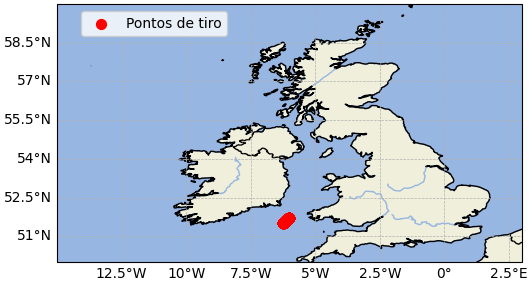
\includegraphics[width=10cm,height=5.5cm]{../imagens/area_de_estudo.png}	
			\tiny{\caption{Localização dos pontos de tiro usando a projeção Plate\newline Carree da biblioteca Cartopy. Ilustração dos 1064 posições de disparo.}} 	
			\label{pontosDeTiro}
		\end{figure}	
	\end{column}
\end{columns}	
	
\end{frame}

% ----------------- NOVO SLIDE --------------------------------	
\begin{frame}{Área de estudo}
\framesubtitle{Litologia típica}	
	
\begin{columns}[onlytextwidth, T]
	\begin{column}{.90\textwidth}
		\begin{figure}[h]
			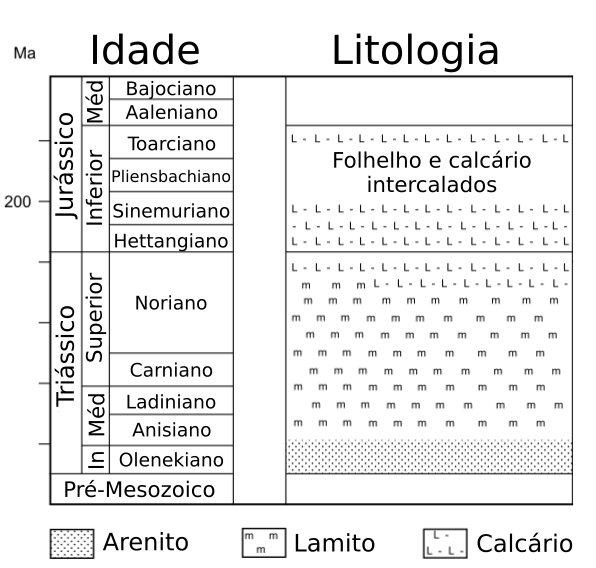
\includegraphics[width=6.7cm,height=5.5cm]{../imagens/regional.png}	
			\tiny{\caption{Carta estratigráfica regional do canal de Bristol, apresentando os tempos 				geológicos e as principais litologias presentes na região \cite{glen2005basin}.}} 	
			\label{litologia}
		\end{figure}	
	\end{column}
\end{columns}	
	
\end{frame}
% ----------------- NOVO SLIDE --------------------------------	
\begin{frame}{Processamento sísmico}
\framesubtitle{Ordenação de traços em ponto médio comum (CMP)}	
	
\pause
\begin{columns}[onlytextwidth, T]
	\begin{column}{.90\textwidth}
		\begin{figure}[h]
			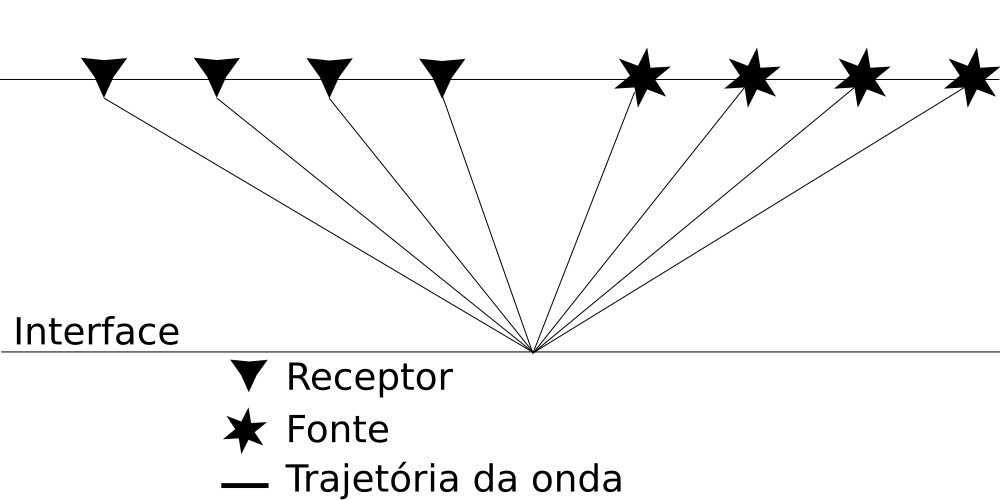
\includegraphics[width=10cm,height=5.5cm]{../imagens/cdp.png}	
			\tiny{\caption{Iluminação do mesmo ponto em profundidade para meios plano-paralelos sem variação lateral de velocidade.}} 	
			\label{cmpDomain}
		\end{figure}	
	\end{column}
\end{columns}	
	
\end{frame}
% ----------------- NOVO SLIDE --------------------------------	
\begin{frame}{Processamento sísmico}
\framesubtitle{Análise de velocidades sísmicas - \citeonline{yilmaz2001seismic}}	
	
\begin{columns}[onlytextwidth, T]
	\begin{column}{.50\textwidth}
		\begin{figure}[h]
			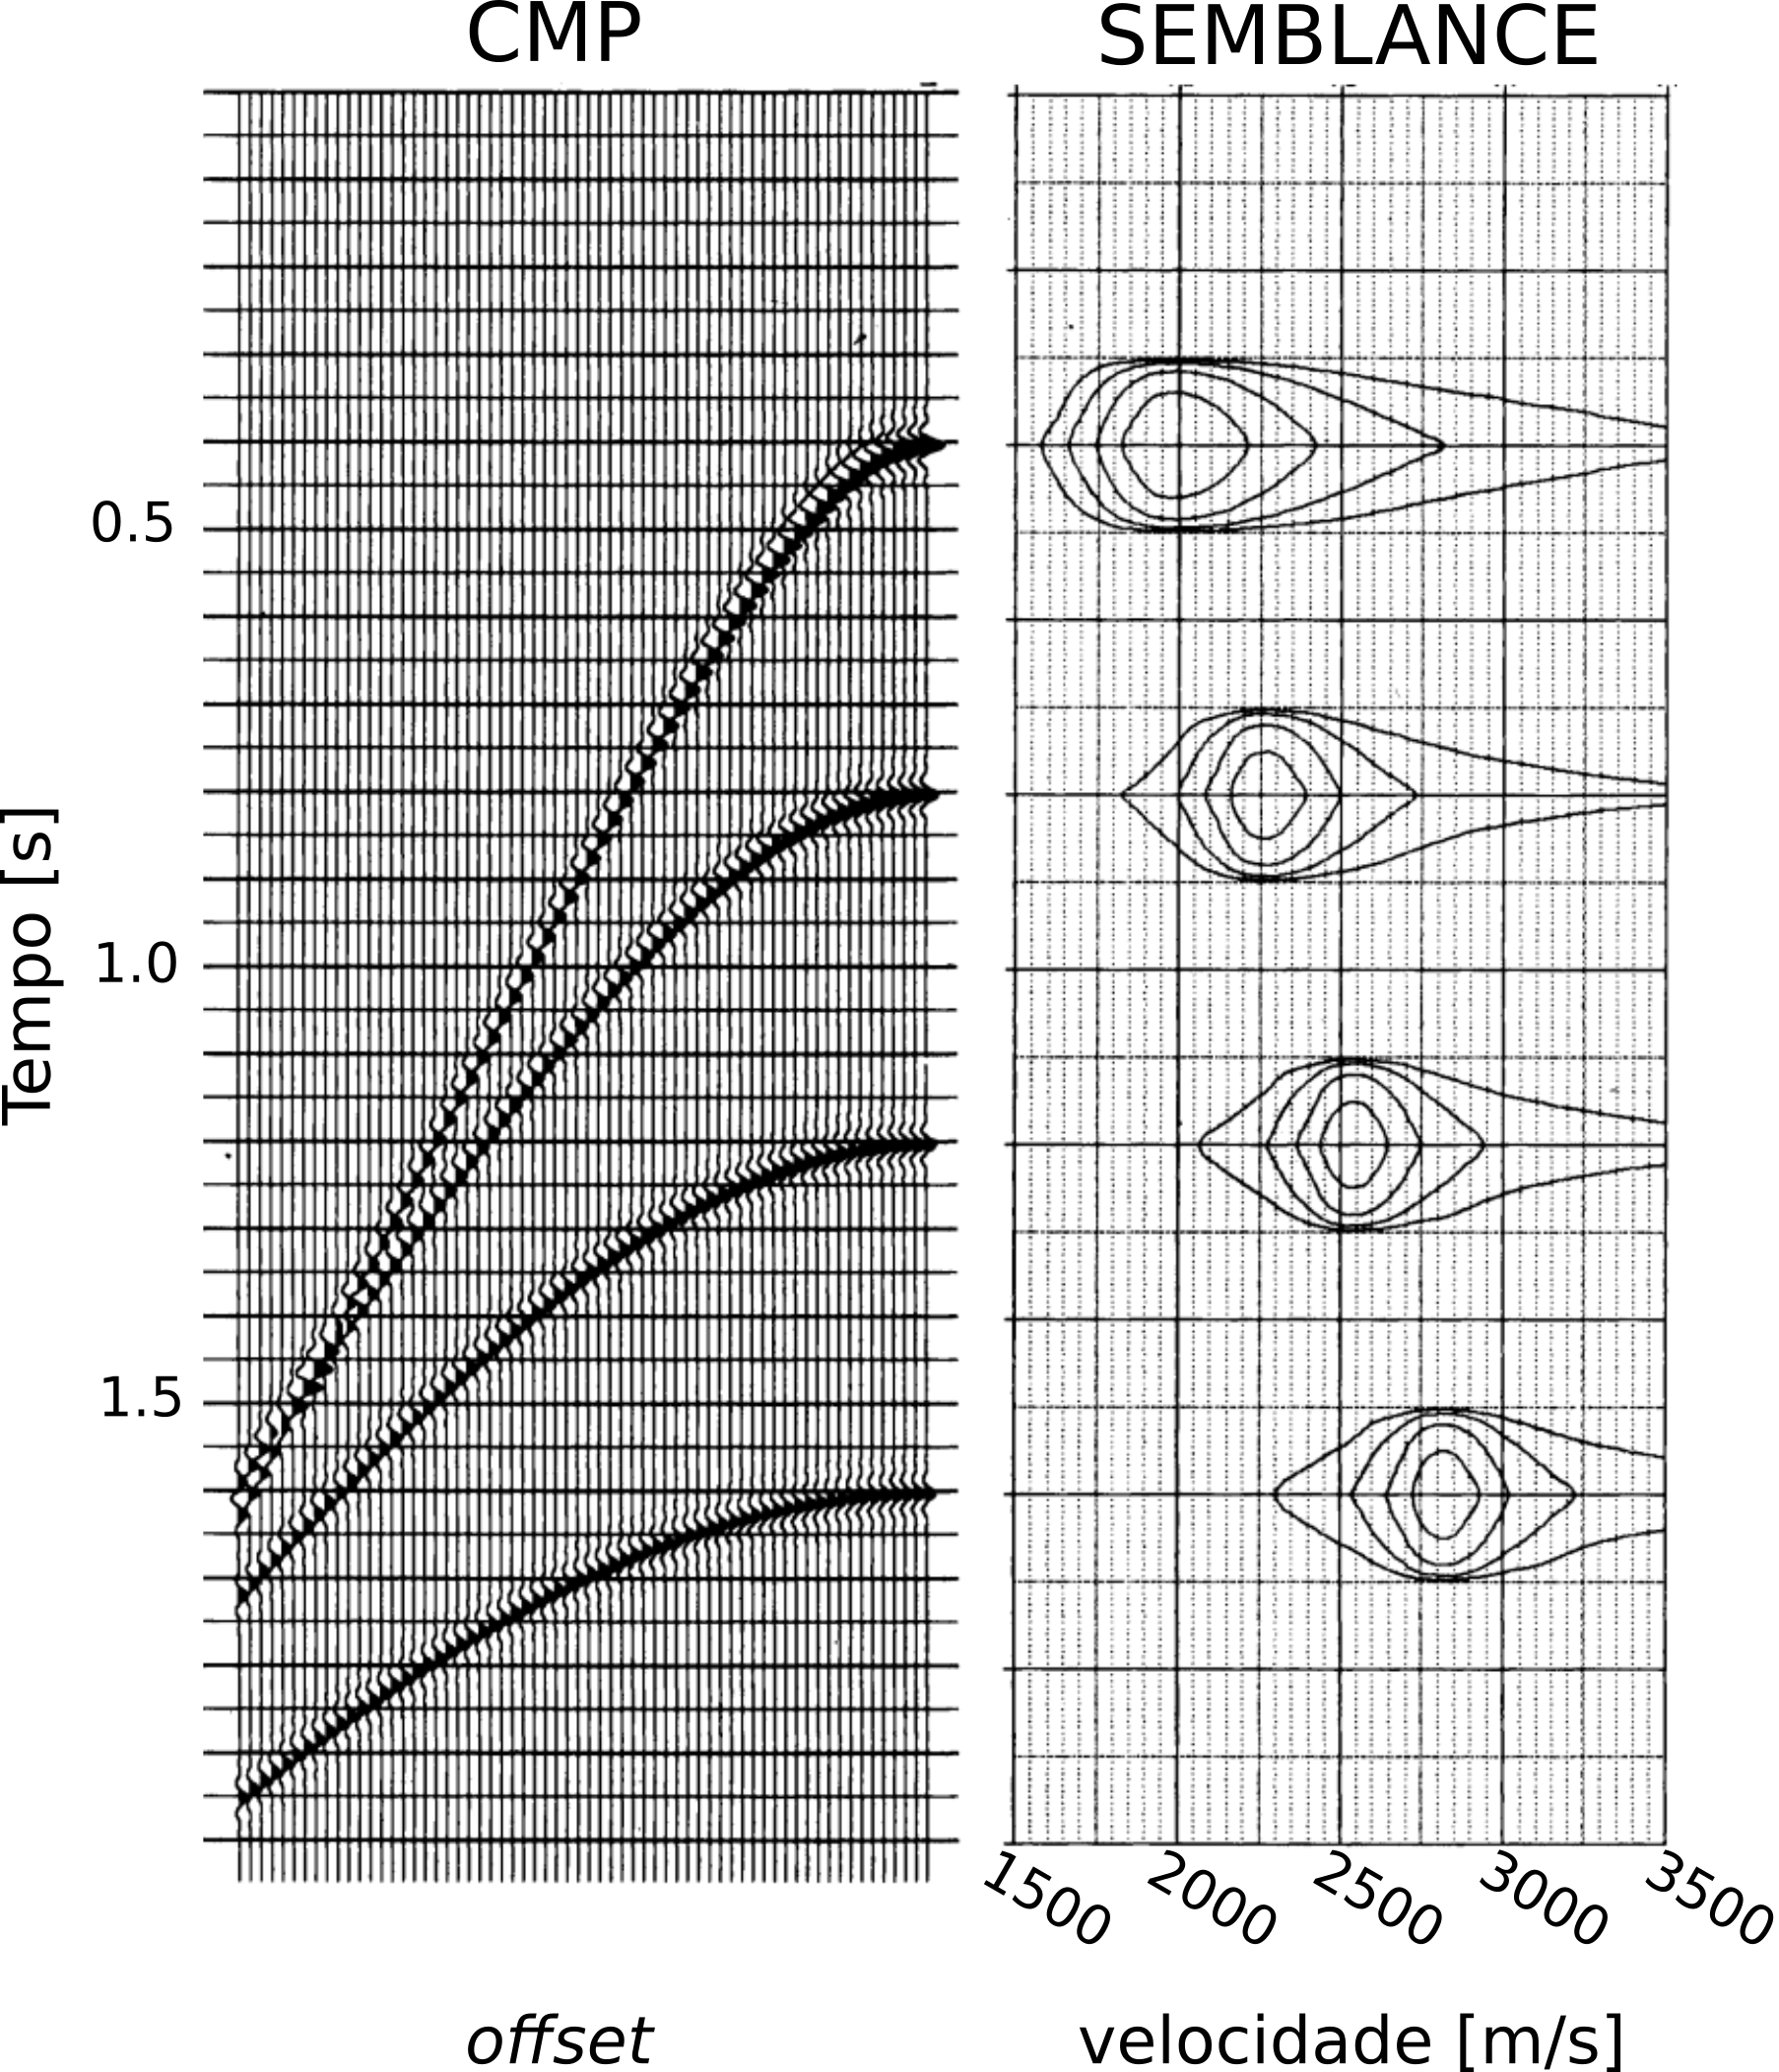
\includegraphics[width=6cm,height=6cm]{../imagens/cmpSemblance.png}	
			\tiny{\caption{Correlação das hipérboles de reflexão (adaptado de \citeonline{yilmaz2001seismic}).}} 	
			\label{velan}
		\end{figure}	
	\end{column}

	\begin{column}{.50\textwidth}
		\begin{equation}
			t^2(x) = t^2_0 + \dfrac{x^2}{v_{NMO}}  
		\end{equation}

		\begin{itemize}
			\small
			\item[$\bullet$] $t(x)\,\,\,\,$ - tempo nas hipérboles; 
			\item[$\bullet$] $t_0\,\,\,\,\,\,\,\,\,$ - tempo de \textit{offset} zero; 
			\item[$\bullet$] $x\,\,\,\,\,\,\,\,\,\,$ - projeção das hipérboles;
			\item[$\bullet$] $v_{NMO}$ - velocidade de ajuste;
			\bigskip\bigskip
			
			\item[$\to$] Encontrar, para cada tempo, a melhor hipérbole que representa a reflexão.
		\end{itemize}
	\end{column}
\end{columns}	
		
\end{frame}
% ----------------- NOVO SLIDE --------------------------------	
\begin{frame}{Processamento sísmico}
\framesubtitle{Empilhamento de dados sísmicos - \citeonline{yilmaz2001seismic}}	

\begin{columns}[onlytextwidth, T]
	\begin{column}{.90\textwidth}
		\begin{figure}[h]
			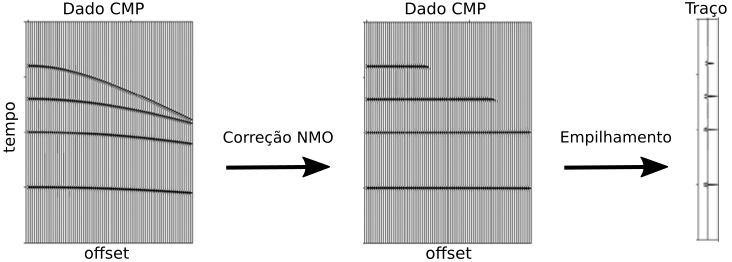
\includegraphics[width=10cm,height=4.7cm]{../imagens/empilhamento.png}	
			\tiny{\caption{Correção \textit{normal move out} e empilhamento para um sismograma de ponto médio comum. Velocidades $v_{NMO}$ estimadas são usadas no processo, transformando um sismograma em um único traço (adaptado de \citeonline{yilmaz2001seismic}).}} 	
			\label{empilhamento}
		\end{figure}	
	\end{column}
\end{columns}	

\end{frame}
% ----------------- NOVO SLIDE --------------------------------	
\begin{frame}{Processamento sísmico}
\framesubtitle{Conversões de velocidades - \citeonline{dix1955seismic}}	

\begin{equation}
	\begin{cases}
		\bigskip V_{INT}[i] =  \sqrt{\left(\dfrac{V_{RMS}^2[i] t_{dt}[i] - V_{RMS}^2[i-1] t_{dt}[i-1]}{t_{dt}[i] - t_{dt}[i-1]}\right)}  \\
		V_{NMO}[i] \approx V_{RMS}[i] = \sqrt{\left(\dfrac{\displaystyle\sum V_{INT}^2[i]t_{di}[i]}{\displaystyle\sum t_{di}[i]}\right)}
		\end{cases}
	\label{dix}
\end{equation}

\bigskip
\begin{itemize}
	\small
	\item[$\bullet$] $V_{INT}[i]$ - Velocidade intervalar presente no meio;
	\smallskip
	\item[$\bullet$] $V_{NMO}[i] \approx V_{RMS}[i]$ - Simplificações matemáticas de velocidade;
	\smallskip
	\item[$\bullet$] $t_{dt}[i]$ - Tempo duplo total;
	\smallskip
	\item[$\bullet$] $t_{di}[i]$ - Tempo duplo intervalar. 
	
	\item[$\to$] A primeira conversão foi realizada para montar o modelo $v_p$.
\end{itemize}

\end{frame}
% ----------------- NOVO SLIDE --------------------------------	
\begin{frame}{Modelagem sísmica}
\framesubtitle{Definições da equação governante}	
	
\pause
\begin{itemize}
	\small
	\item[$\to$] Equação da onda para meios elásticos isotrópicos de campo duplo $\vec{v}$  e $\vec{\sigma}$ \citeonline{virieux1986p} e \citeonline{levander1988fourth}.
	\smallskip\smallskip\smallskip\smallskip\smallskip\smallskip\smallskip
	
	\pause
	\item[$\to$] Apesar da equação possuir componentes vetoriais, somente o campo escalar de pressão foi utilizado. 
	\smallskip\smallskip\smallskip\smallskip\smallskip\smallskip\smallskip
	
	\pause
	\item[$\to$] Resolução numérica através do método das diferenças finitas utilizando malha intercalada para melhor propagação em interfaces água sedimento. 
	\smallskip\smallskip\smallskip\smallskip\smallskip\smallskip\smallskip
	
	\pause
	\item[$\to$] Operadores de diferenças finitas em 8E2T utilizando stencil centrado nas tensões normais.    
\end{itemize}	
	
\end{frame}
% ----------------- NOVO SLIDE --------------------------------	
\begin{frame}{Modelagem sísmica}
\framesubtitle{Informações gerais}	

\begin{itemize}
	\small
 	
	\item[$\to$] Revisão de \citeonline{virieux1986p} e \citeonline{moczo2000stability}, para averiguar a estabilidade e dispersão numéricos em operadores de diferenças finitas.
	\smallskip\smallskip\smallskip\smallskip\smallskip\smallskip\smallskip
	
	\pause
	\item[$\to$] Equação de \citeonline{cerjan1985nonreflecting} foi aplicada nas bordas dos modelos, \newline para simular um meio infinito.  
	\smallskip\smallskip\smallskip\smallskip\smallskip\smallskip\smallskip
	
	\pause
	\item[$\to$] Operações de filtragem na fonte sísmica aplicada, no domínio do tempo e da frequência, para se enxergar uma wavelet Ricker no domínio do campo de onda (experimento no texto detalhando os processos). 
\end{itemize}	
	
\end{frame}
% ----------------- NOVO SLIDE --------------------------------	
\section{Metodologia}
\begin{frame}{}
	\bigskip\bigskip\bigskip\bigskip\bigskip\bigskip
	\begin{center}
		\Huge Metodologia
	\end{center}    
\end{frame}
% ----------------- NOVO SLIDE --------------------------------	
\begin{frame}{Características do dado sísmico}
\framesubtitle{Informações gerais - \textit{Oil and Gas Authority}, instituição do Reino Unido}	

\begin{columns}[onlytextwidth, T]
	\begin{column}{.5\textwidth}
		\begin{itemize}
			\small
			\item[$\to$] Geometria: \textit{End On}
			\item[$\bullet$] 1064 estações de tiros
			\item[$\bullet$] 320 receptores ativos por tiro
		\end{itemize}
		
		\bigskip
		\begin{itemize}
			\small
			\item[$\to$] Temporais:
			\item[$\bullet$] 2300 amostras
			\item[$\bullet$] 4 $ms$ de discretização
			\item[$\bullet$] 9,20 $s$ de tempo total
		\end{itemize}
		
		\bigskip
		\begin{itemize}
			\small
			\item[$\to$] Armazenamento:
			\item[$\bullet$] 3,2 GB de ocupação em disco
		\end{itemize}		
	\end{column}

	\begin{column}{.5\textwidth}
		\begin{itemize}
			\small
			\item[$\to$] Espaciais:
			\item[$\bullet$] 100 m de \textit{offset} mínimo
			\item[$\bullet$] 8 km de \textit{spread} 	
			\item[$\bullet$] 25 m entre receptores
			\item[$\bullet$] 25 m entre fontes
			\item[$\bullet$] 22650 m de cobertura sísmica
			\item[$\bullet$] 34650 m de aquisição sísmica
		\end{itemize}		
	\end{column}
\end{columns}

\end{frame}
% ----------------- NOVO SLIDE --------------------------------	
\begin{frame}{Construção do modelo de velocidades $v_p$}
	\framesubtitle{Entendendo a geometria da aquisição para gerar o modelo}	
	
	\pause	
	\begin{columns}[onlytextwidth, T]
		\begin{column}{.9\textwidth}
			\begin{figure}[h]
				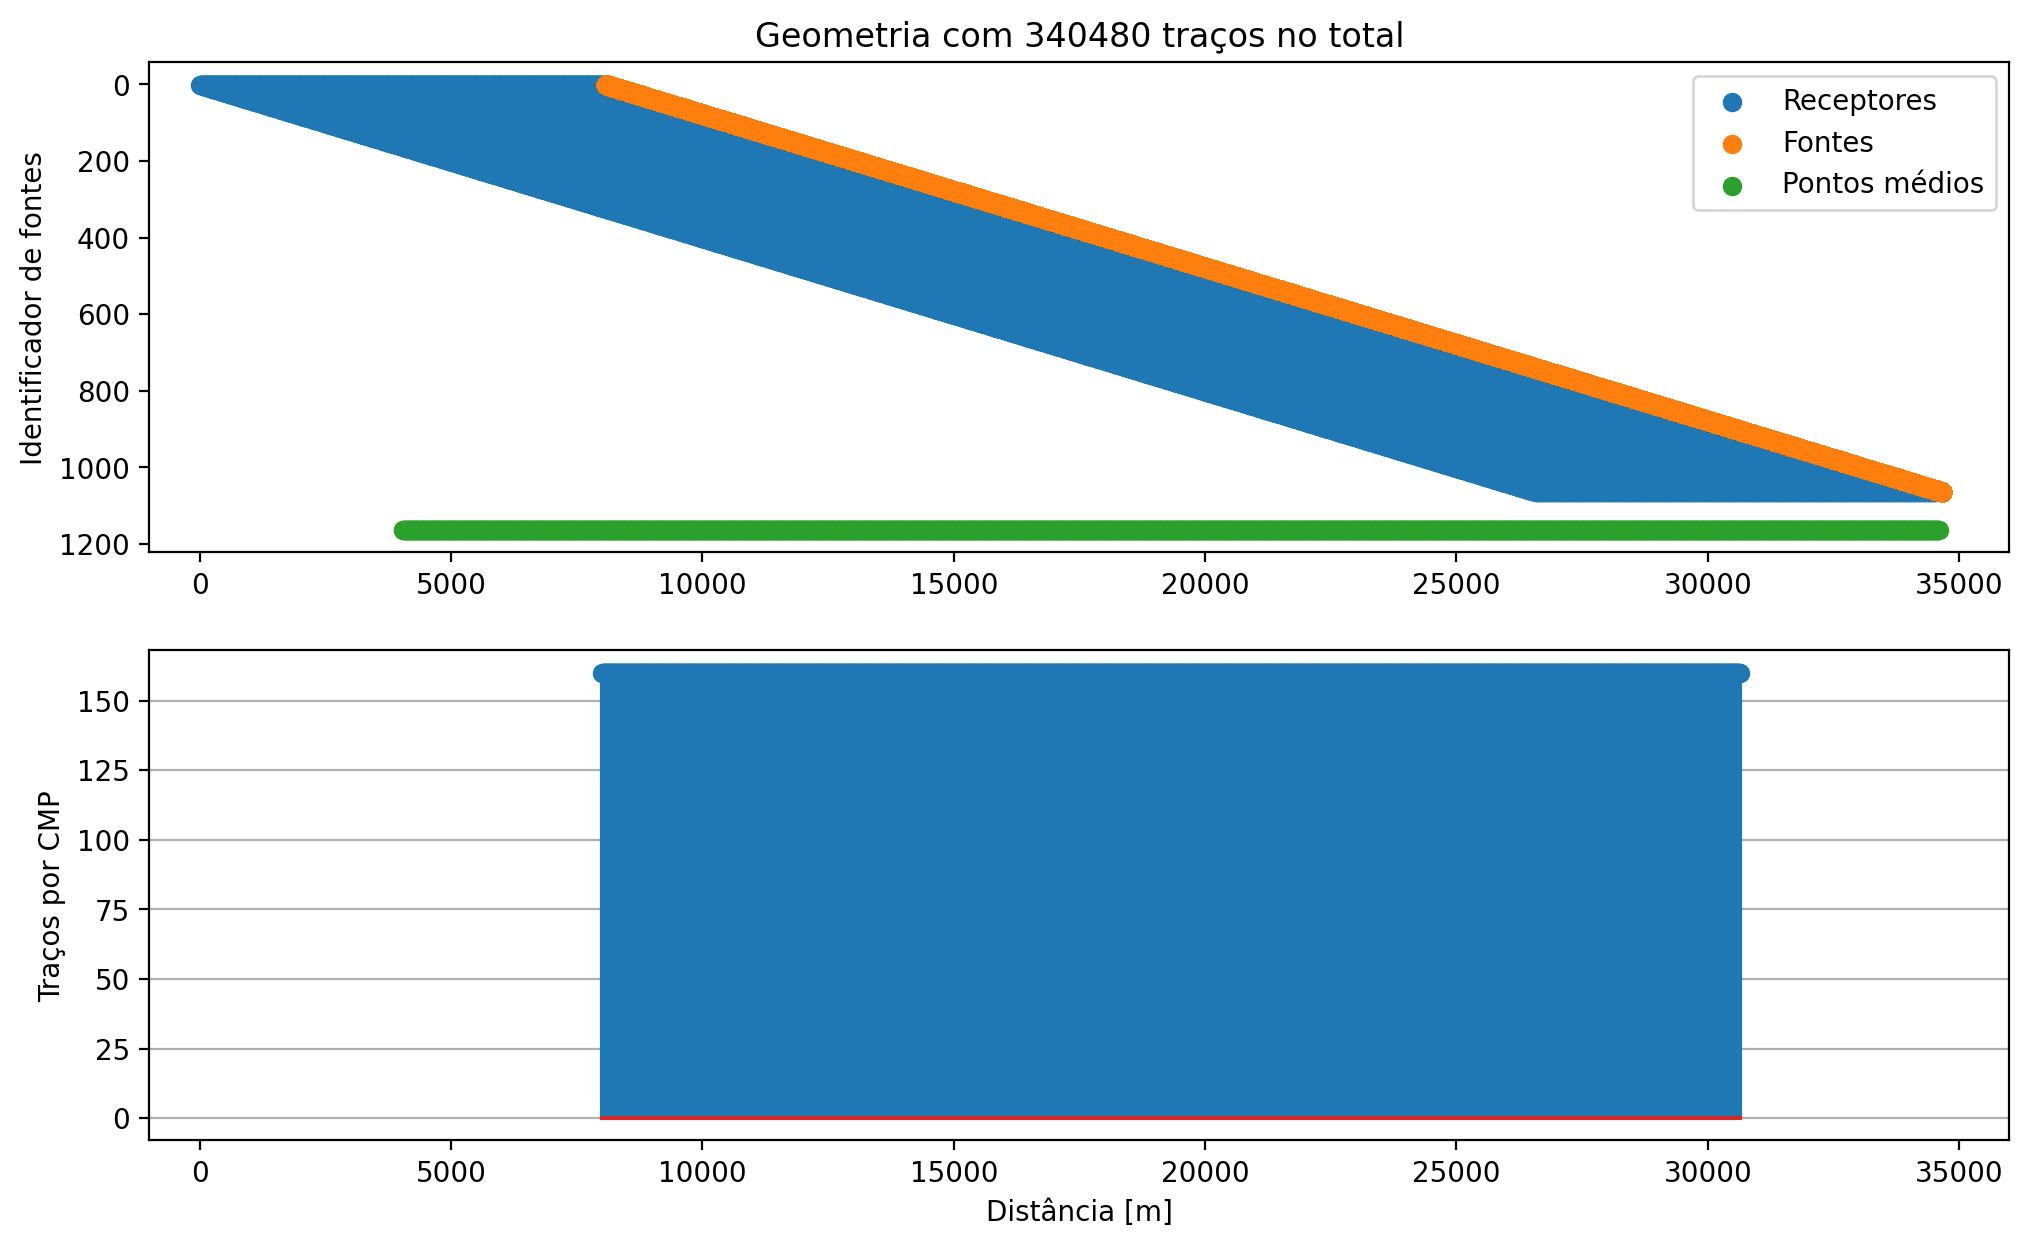
\includegraphics[width=10cm,height=6cm]{../imagens/cmpTraceCountFullFold.png}	
				\tiny{\caption{Projeção dos CMPs de varredura sísmica completa.}} 	
			\end{figure}			
		\end{column}
	\end{columns}	
	
\end{frame}
% ----------------- NOVO SLIDE --------------------------------	
\begin{frame}{Construção do modelo de velocidades $v_p$}
\framesubtitle{CMPs escolhidos para realização da análise de velocidades}	
		
\begin{columns}[onlytextwidth, T]
	\begin{column}{.9\textwidth}
		\begin{figure}[h]
			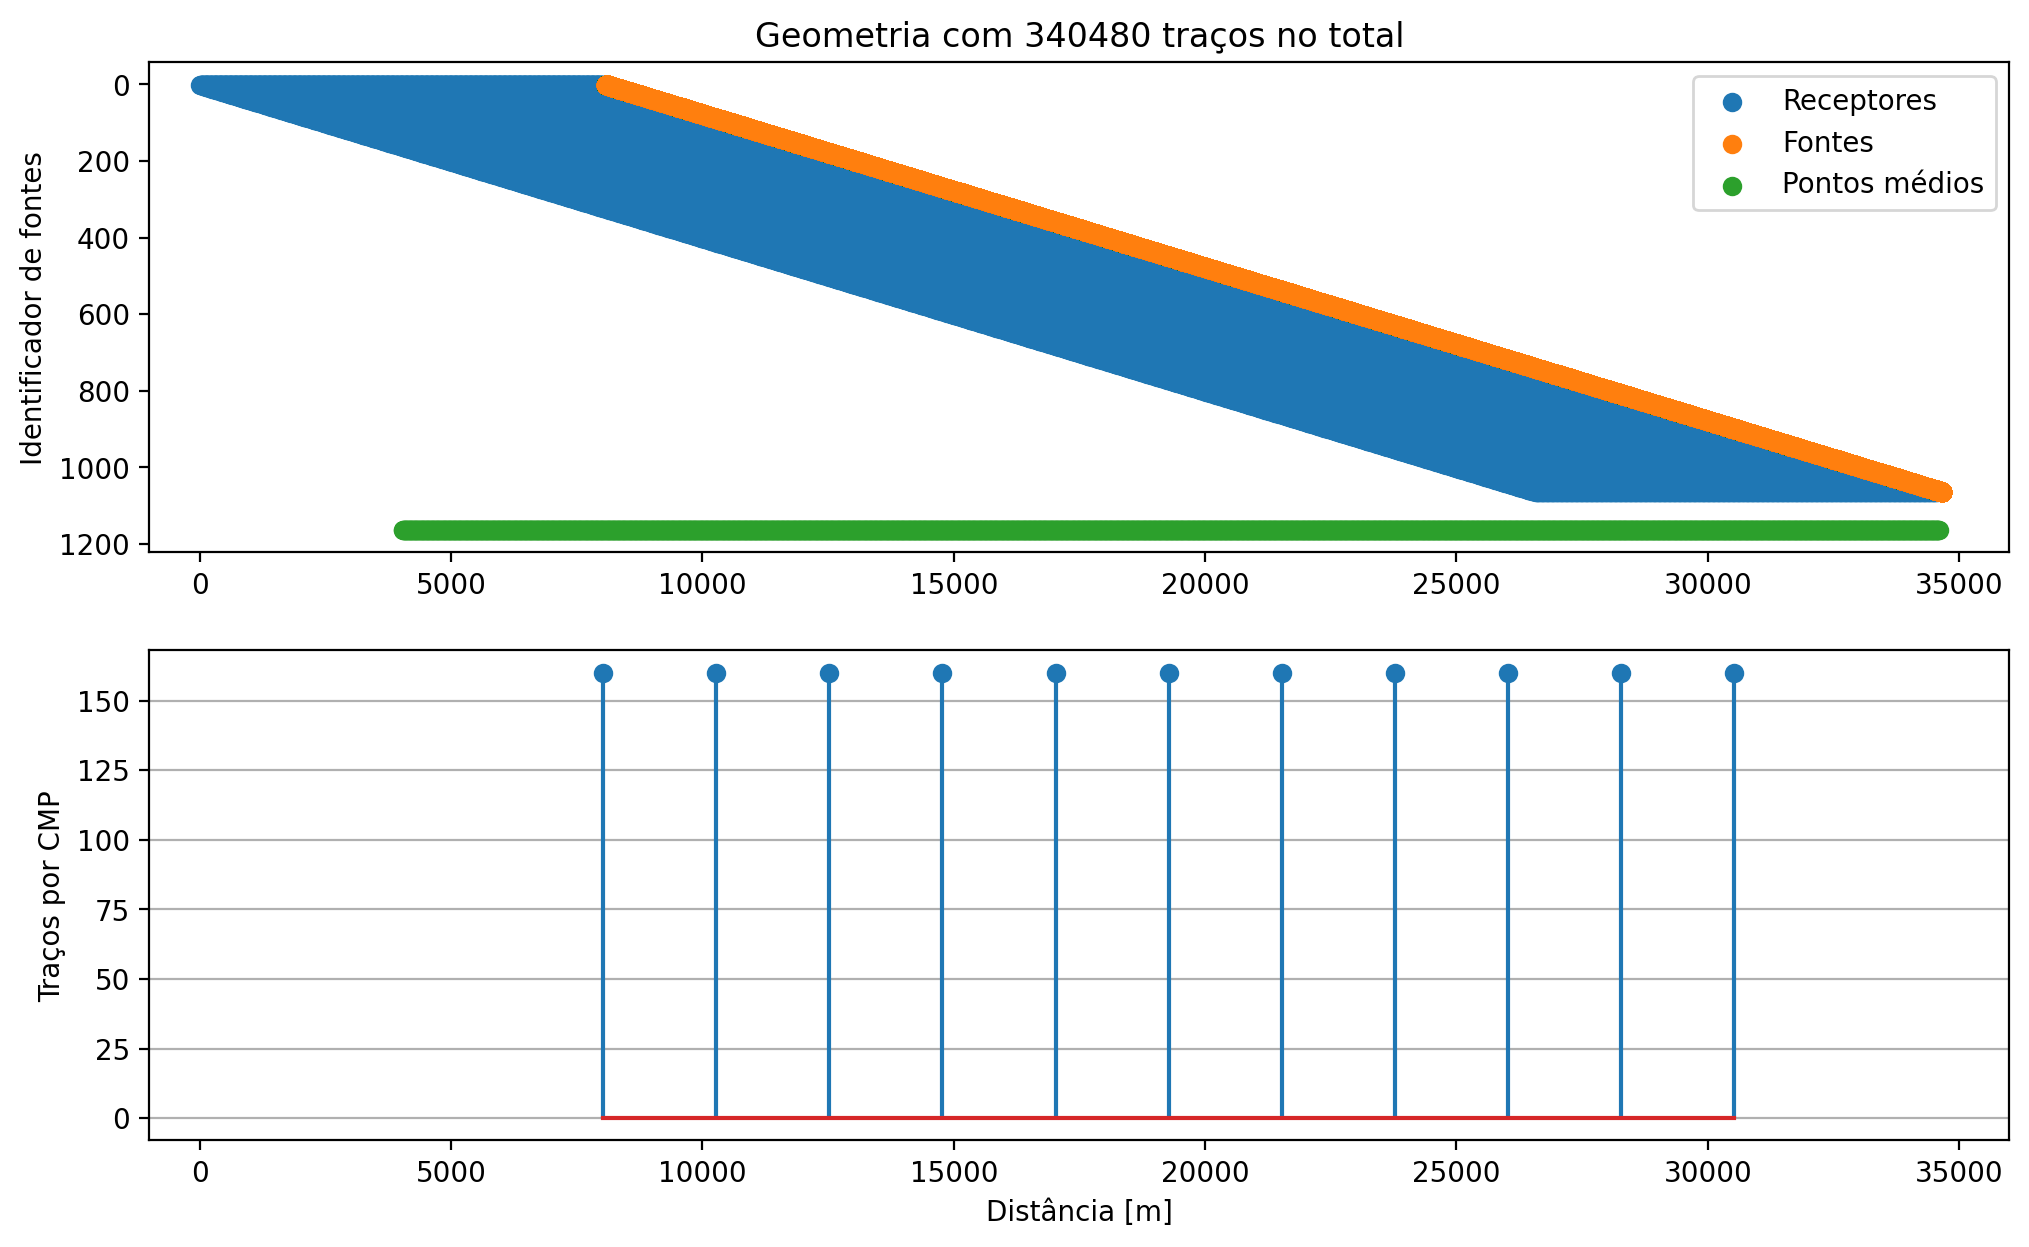
\includegraphics[width=10cm,height=6cm]{../imagens/cmpTraceCountVelAn.png}	
			\tiny{\caption{Escolha regular dos CMPs, espaçados de 2250 m para gerar um modelo suave.}} 	
		\end{figure}			
	\end{column}
\end{columns}	
	
\end{frame}
% ----------------- NOVO SLIDE --------------------------------	
\begin{frame}{Construção do modelo de velocidades $v_p$}
\framesubtitle{Análise de velocidades sísmicas - iva.sh: \textit{Iteractive Velocity Analysis}}	
		
\begin{columns}[onlytextwidth, T]
	\begin{column}{.9\textwidth}
		\begin{figure}[h]
			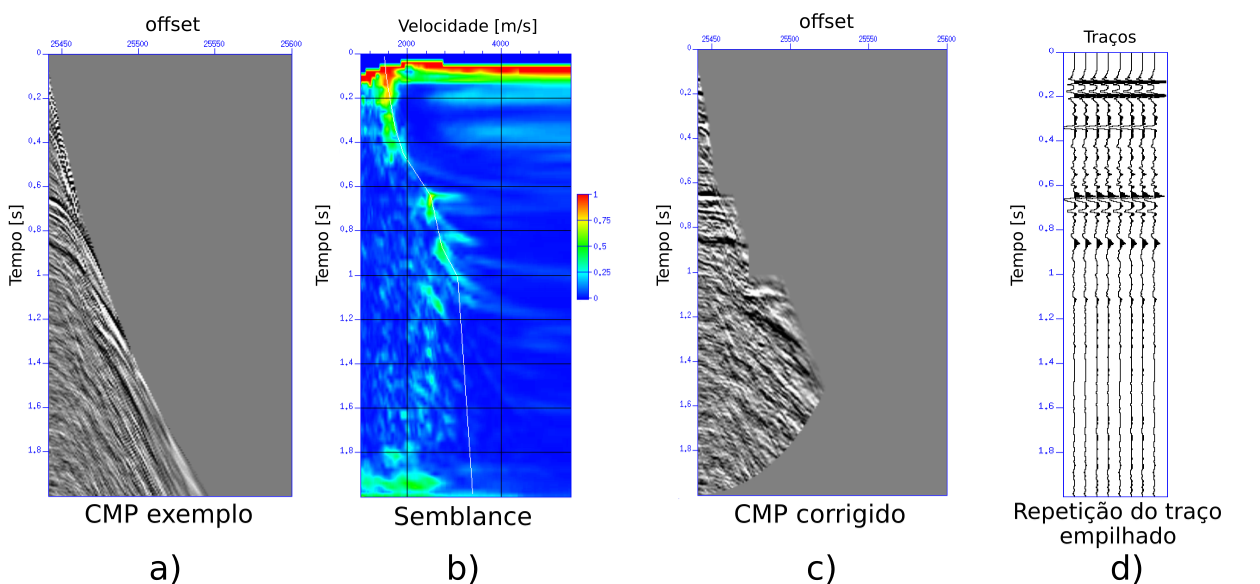
\includegraphics[width=10cm,height=5cm]{../imagens/processamentoReal.png}	
			\tiny{\caption{Utilização do algoritmo encontrado em \citeonline{forel2005seismic}, para realizar as estimativas do campo de velocidades.}} 	
		\end{figure}			
	\end{column}
\end{columns}	
	
\end{frame}
% ----------------- NOVO SLIDE --------------------------------	
\begin{frame}{Construção do modelo de velocidades $v_p$}
	\framesubtitle{Velocidades RMS com maior correlação}	
	
	\begin{columns}[onlytextwidth, T]
		\begin{column}{.9\textwidth}
			\begin{figure}[h]
				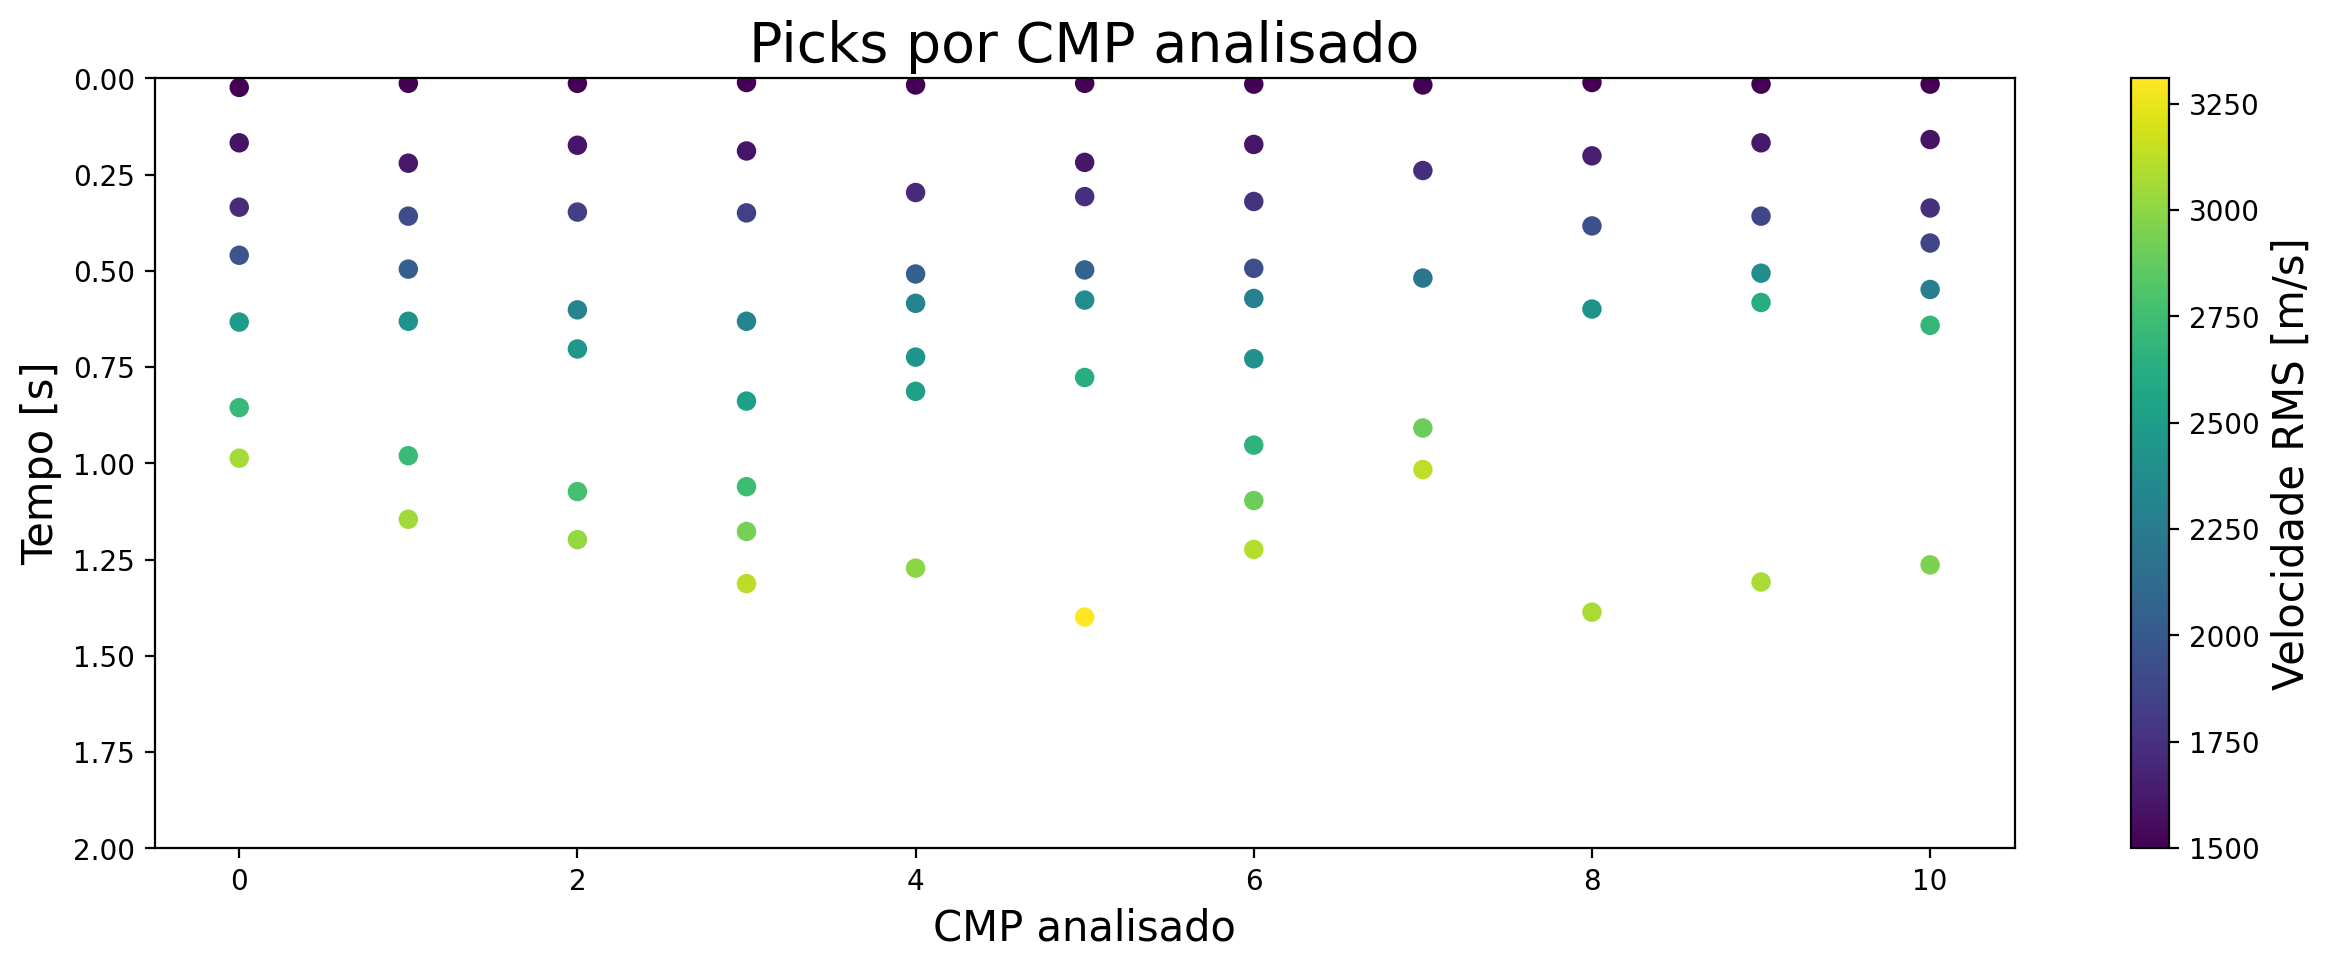
\includegraphics[width=11cm,height=5cm]{../imagens/picksFocado.png}	
				\tiny{\caption{Velocidades estimadas utilizando os CMPs selecionados.}} 	
			\end{figure}			
		\end{column}
	\end{columns}	
	
\end{frame}
% ----------------- NOVO SLIDE --------------------------------	
\begin{frame}{Construção do modelo de velocidades $v_p$}
	\framesubtitle{Interpolação linear irregular no tempo}	
		
	\begin{columns}[onlytextwidth, T]
		\begin{column}{.9\textwidth}
			\begin{figure}[h]
				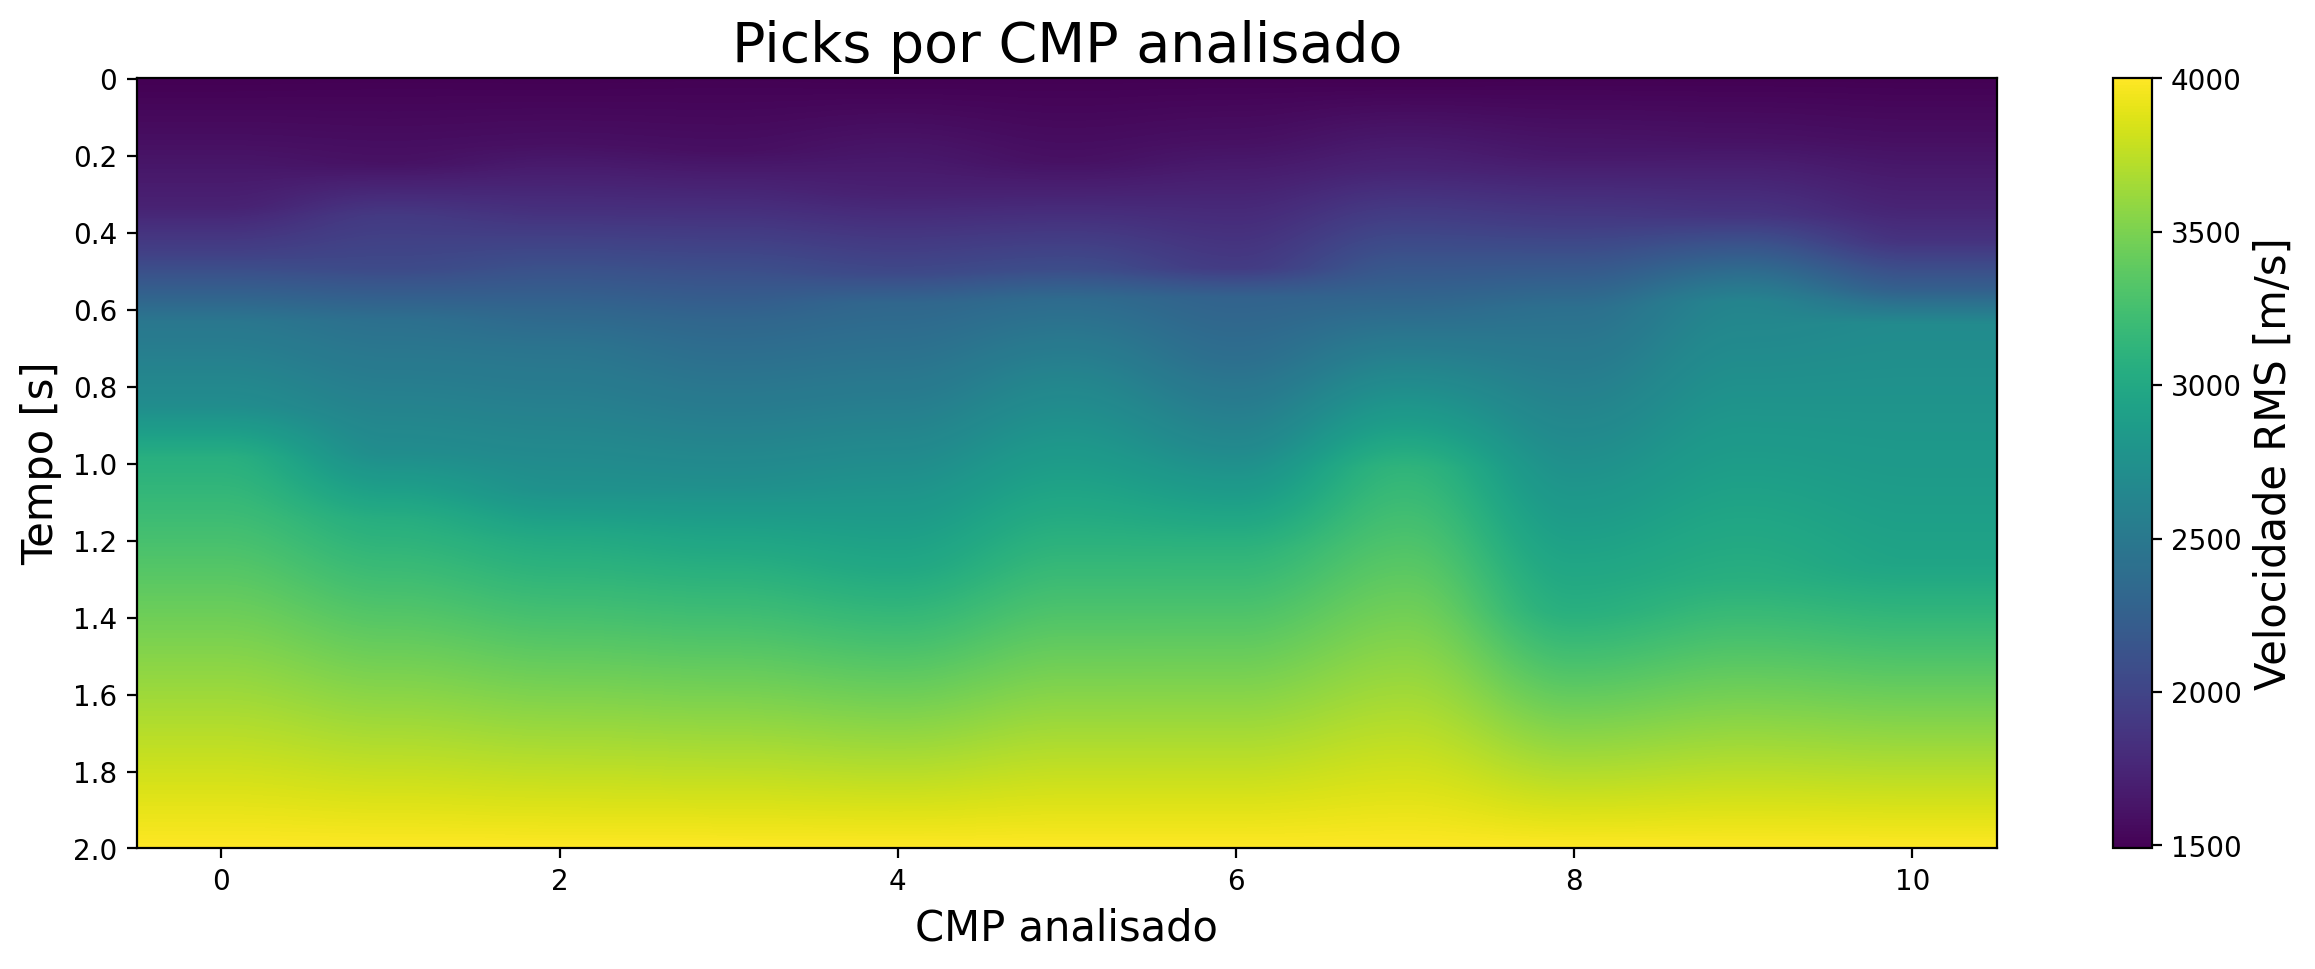
\includegraphics[width=11cm,height=5cm]{../imagens/picksInterpVertical.png}	
				\tiny{\caption{Interpolação no tempo das velocidades RMS.}} 	
			\end{figure}			
		\end{column}
	\end{columns}	
	
\end{frame}
% ----------------- NOVO SLIDE --------------------------------	
\begin{frame}{Construção do modelo de velocidades $v_p$}
	\framesubtitle{Interpolação linear regular no eixo x}	
	
	\begin{columns}[onlytextwidth, T]
		\begin{column}{.9\textwidth}
			\begin{figure}[h]
				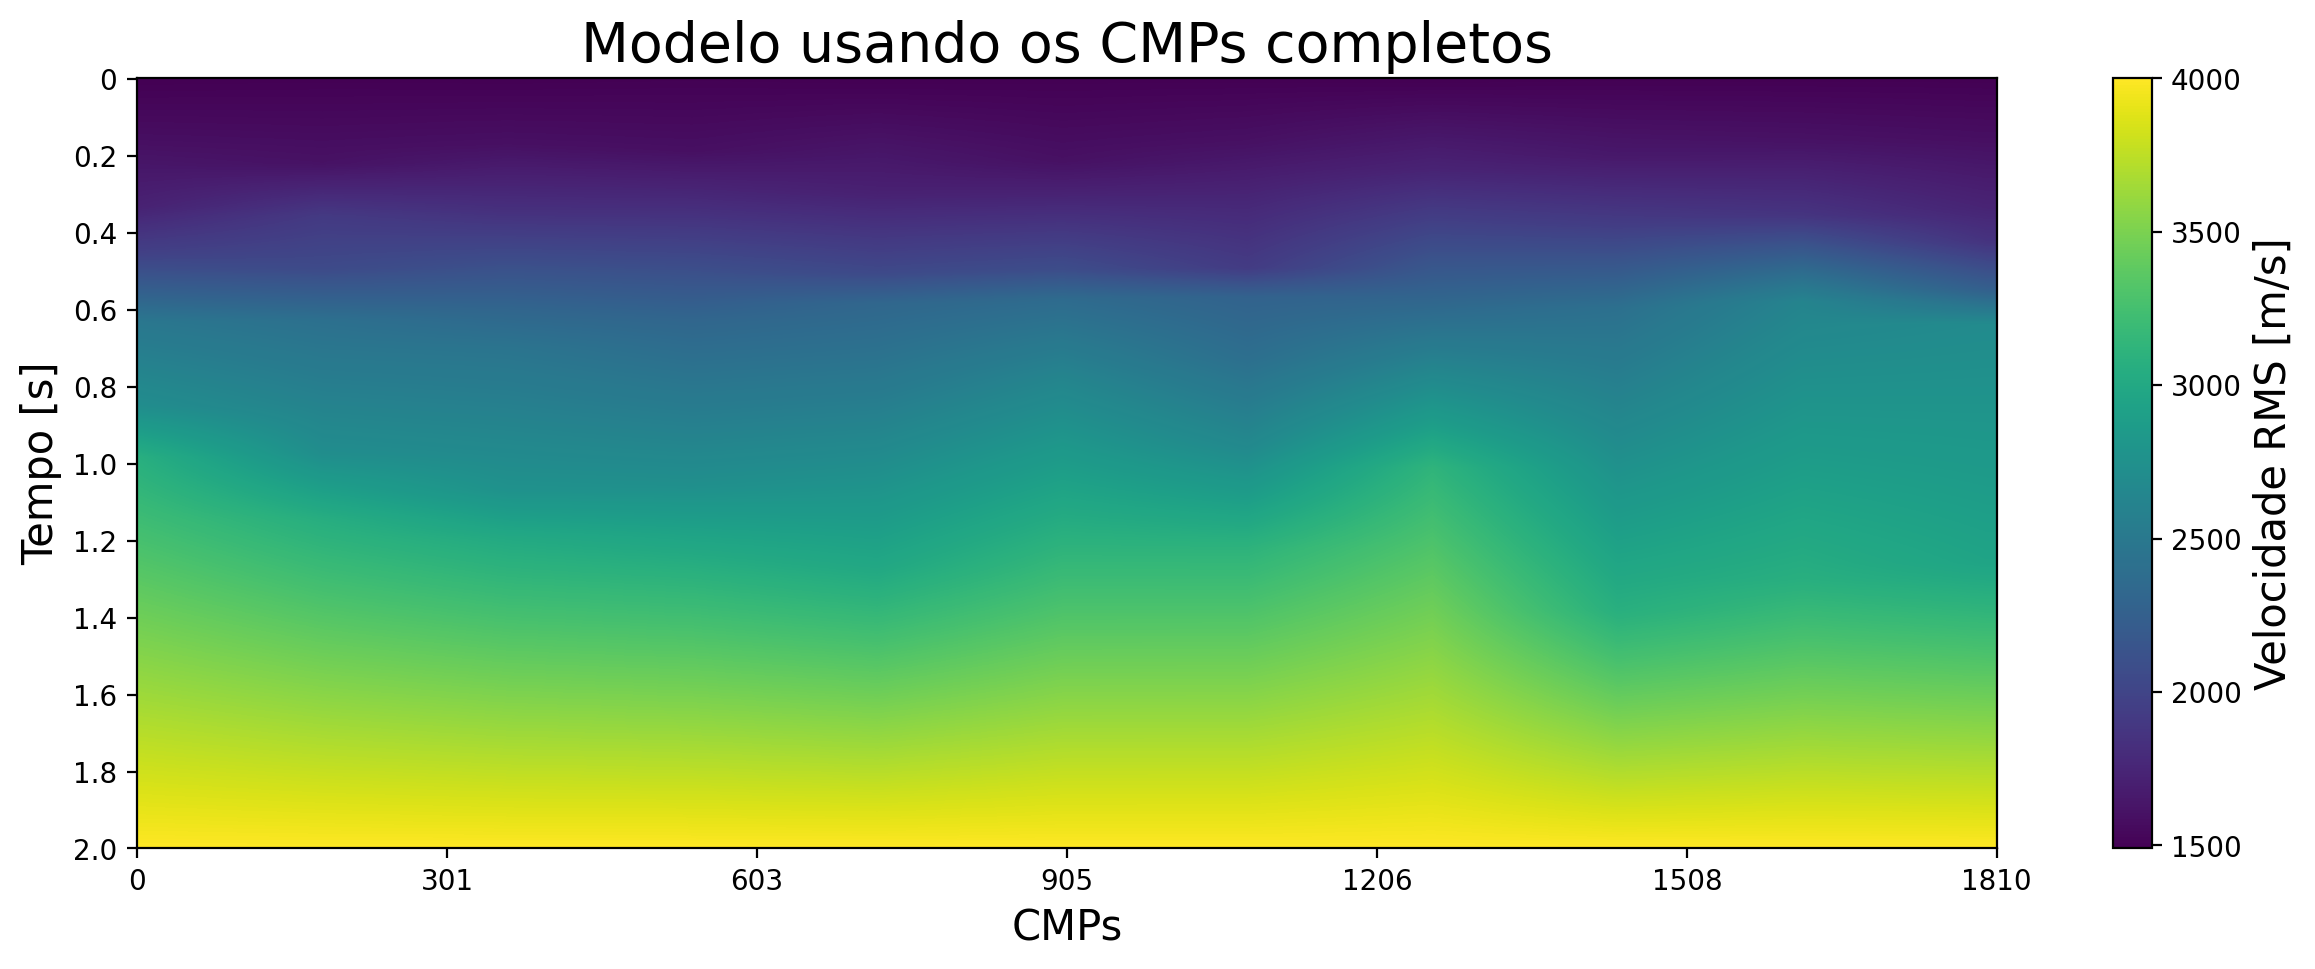
\includegraphics[width=11cm,height=5cm]{../imagens/modeloCompleto.png}	
				\tiny{\caption{Interpolação no espaço das velocidades RMS.}} 	
			\end{figure}			
		\end{column}
	\end{columns}	
	
\end{frame}
% ----------------- NOVO SLIDE --------------------------------	
\begin{frame}{Construção do modelo de velocidades $v_p$}
	\framesubtitle{Suavização da vagarosidade RMS}	
		
	\begin{columns}[onlytextwidth, T]
		\begin{column}{.9\textwidth}
			\begin{figure}[h]
				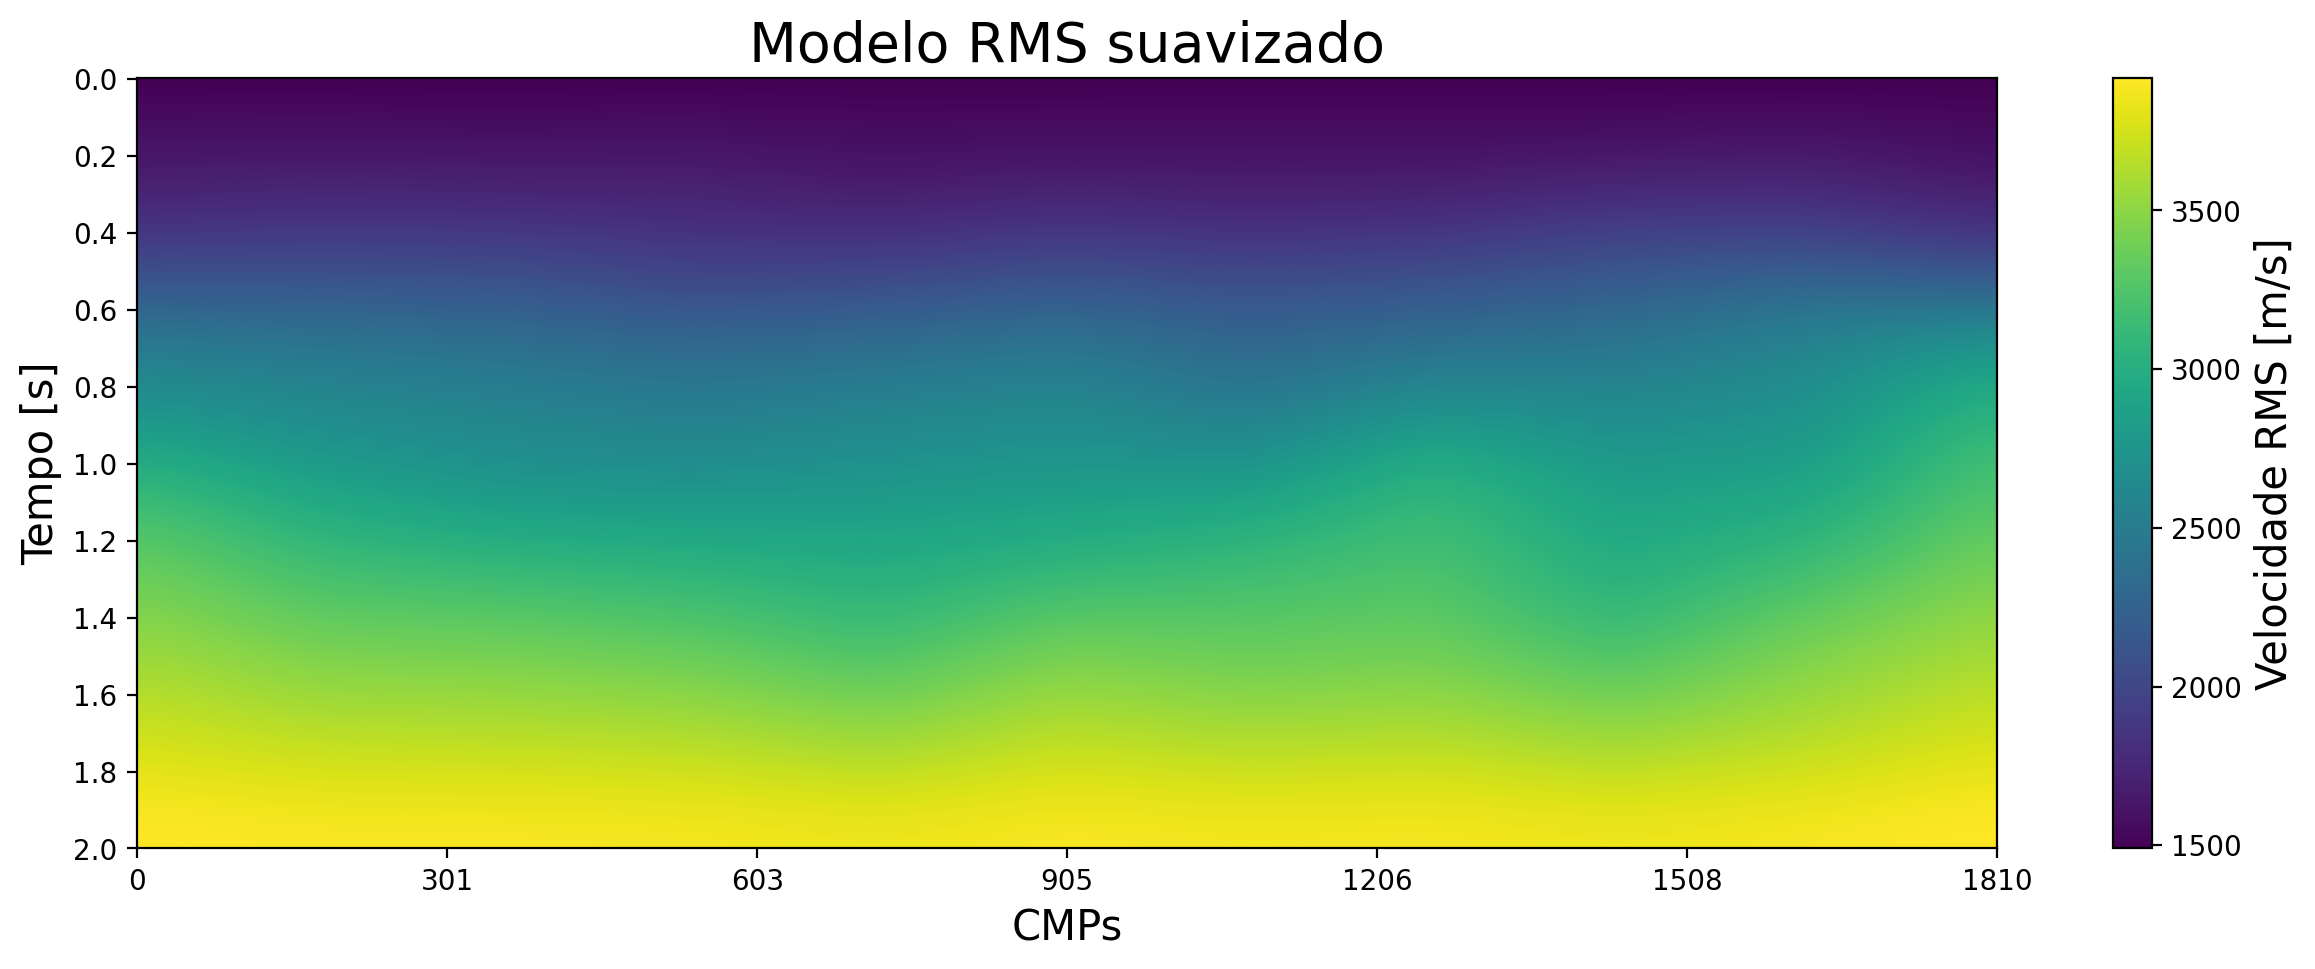
\includegraphics[width=11cm,height=5cm]{../imagens/modeloSuavizadoRMS.png}	
				\tiny{\caption{Modelo RMS suavizado utilizando a função \textit{smooth2} do Seismic Unix com parâmetros 10 para ambas as direções.}} 	
			\end{figure}			
		\end{column}
	\end{columns}	
	
\end{frame}
% ----------------- NOVO SLIDE --------------------------------	
\begin{frame}{Construção do modelo de velocidades $v_p$}
	\framesubtitle{Conversão de velocidade RMS para Intervalar}	
		
	\begin{columns}[onlytextwidth, T]
		\begin{column}{.9\textwidth}
			\begin{figure}[h]
				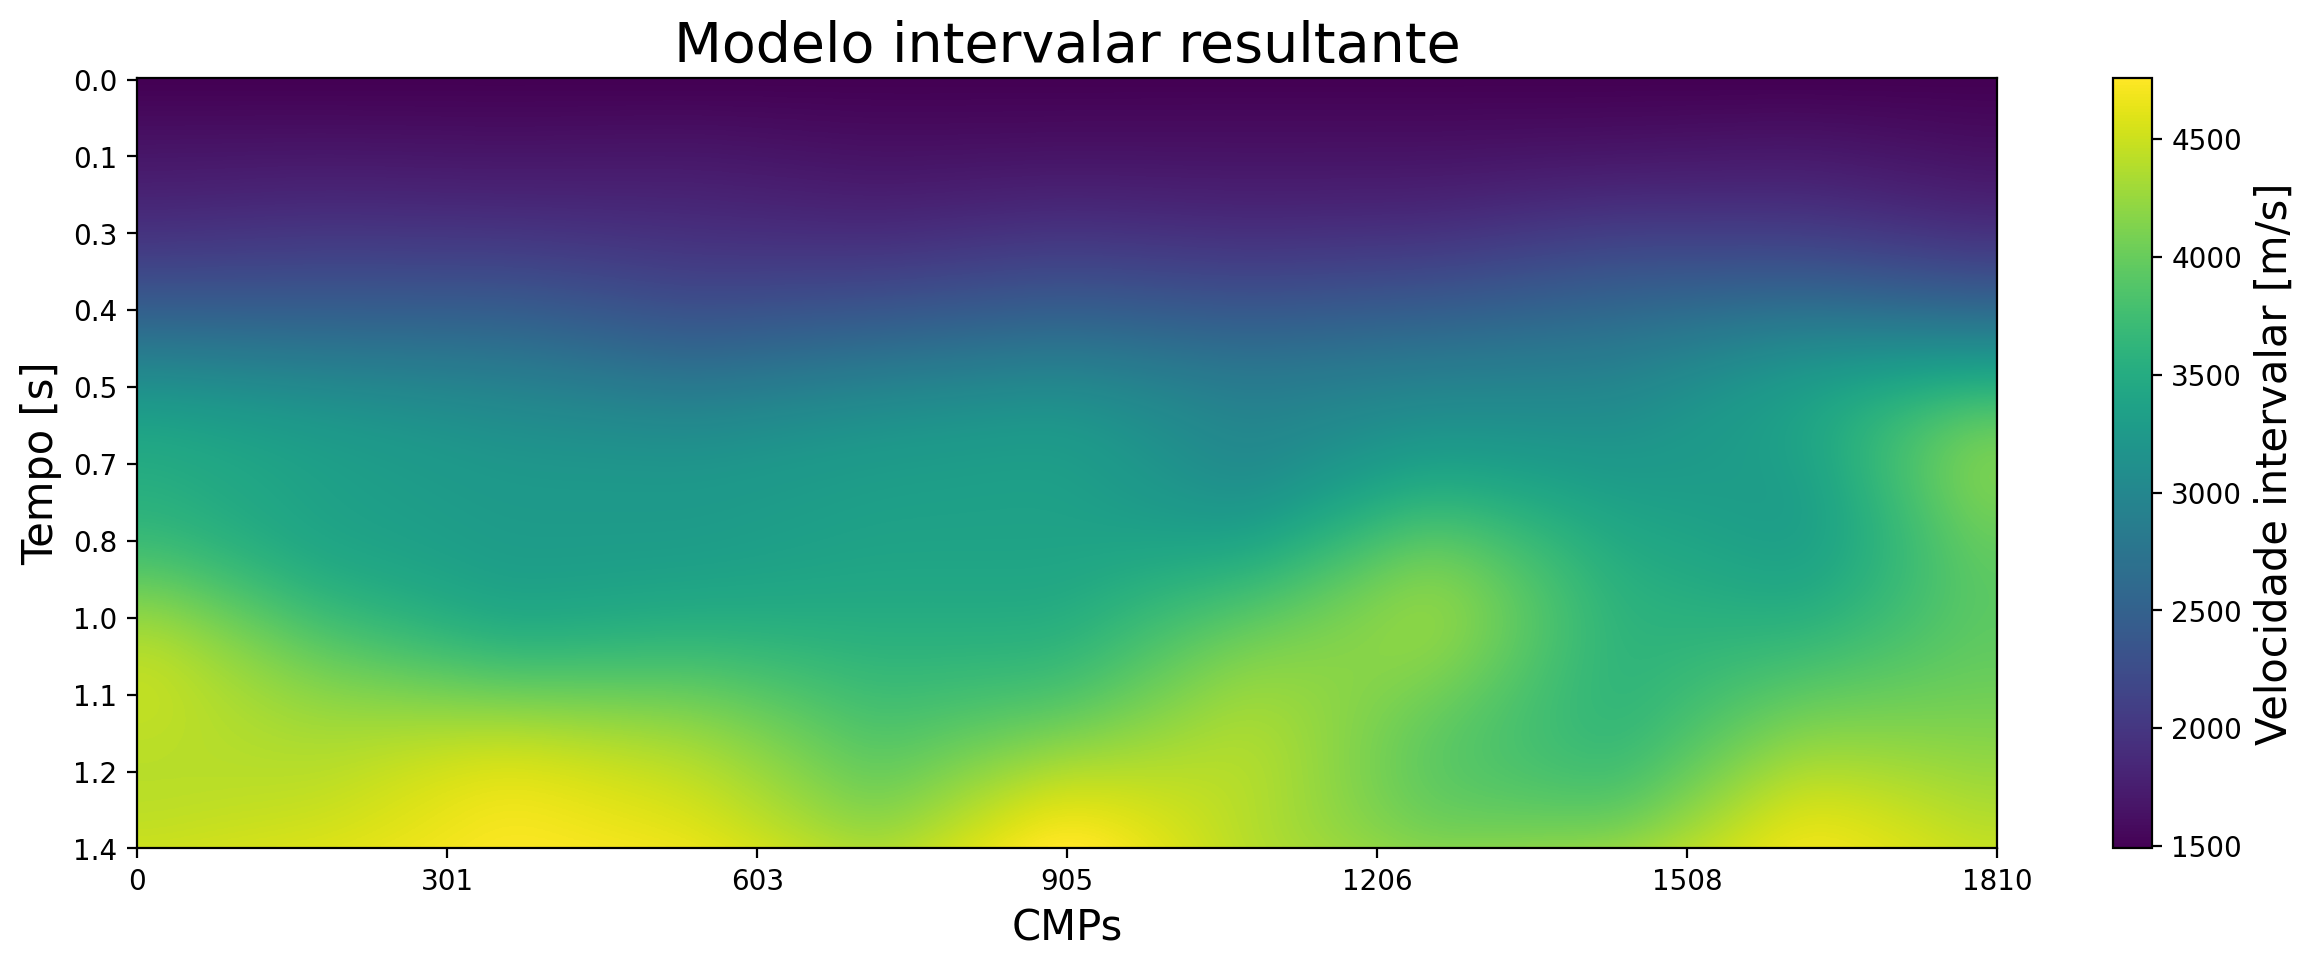
\includegraphics[width=11cm,height=5cm]{../imagens/modeloSuavizadoINTUTIL.png}	
				\tiny{\caption{Modelo convertido para velocidade intervalar em tempo, cortado até 1,4 segundos para otimizar o processo de modelagem.}} 	
			\end{figure}			
		\end{column}
	\end{columns}	
	
\end{frame}
% ----------------- NOVO SLIDE --------------------------------	
\begin{frame}{Construção do modelo de velocidades $v_p$}
	\framesubtitle{Encaixe do modelo $v_p$ na geometria de aquisição}	
	
	\begin{columns}[onlytextwidth, T]
		\begin{column}{.9\textwidth}
			\begin{figure}[h]
				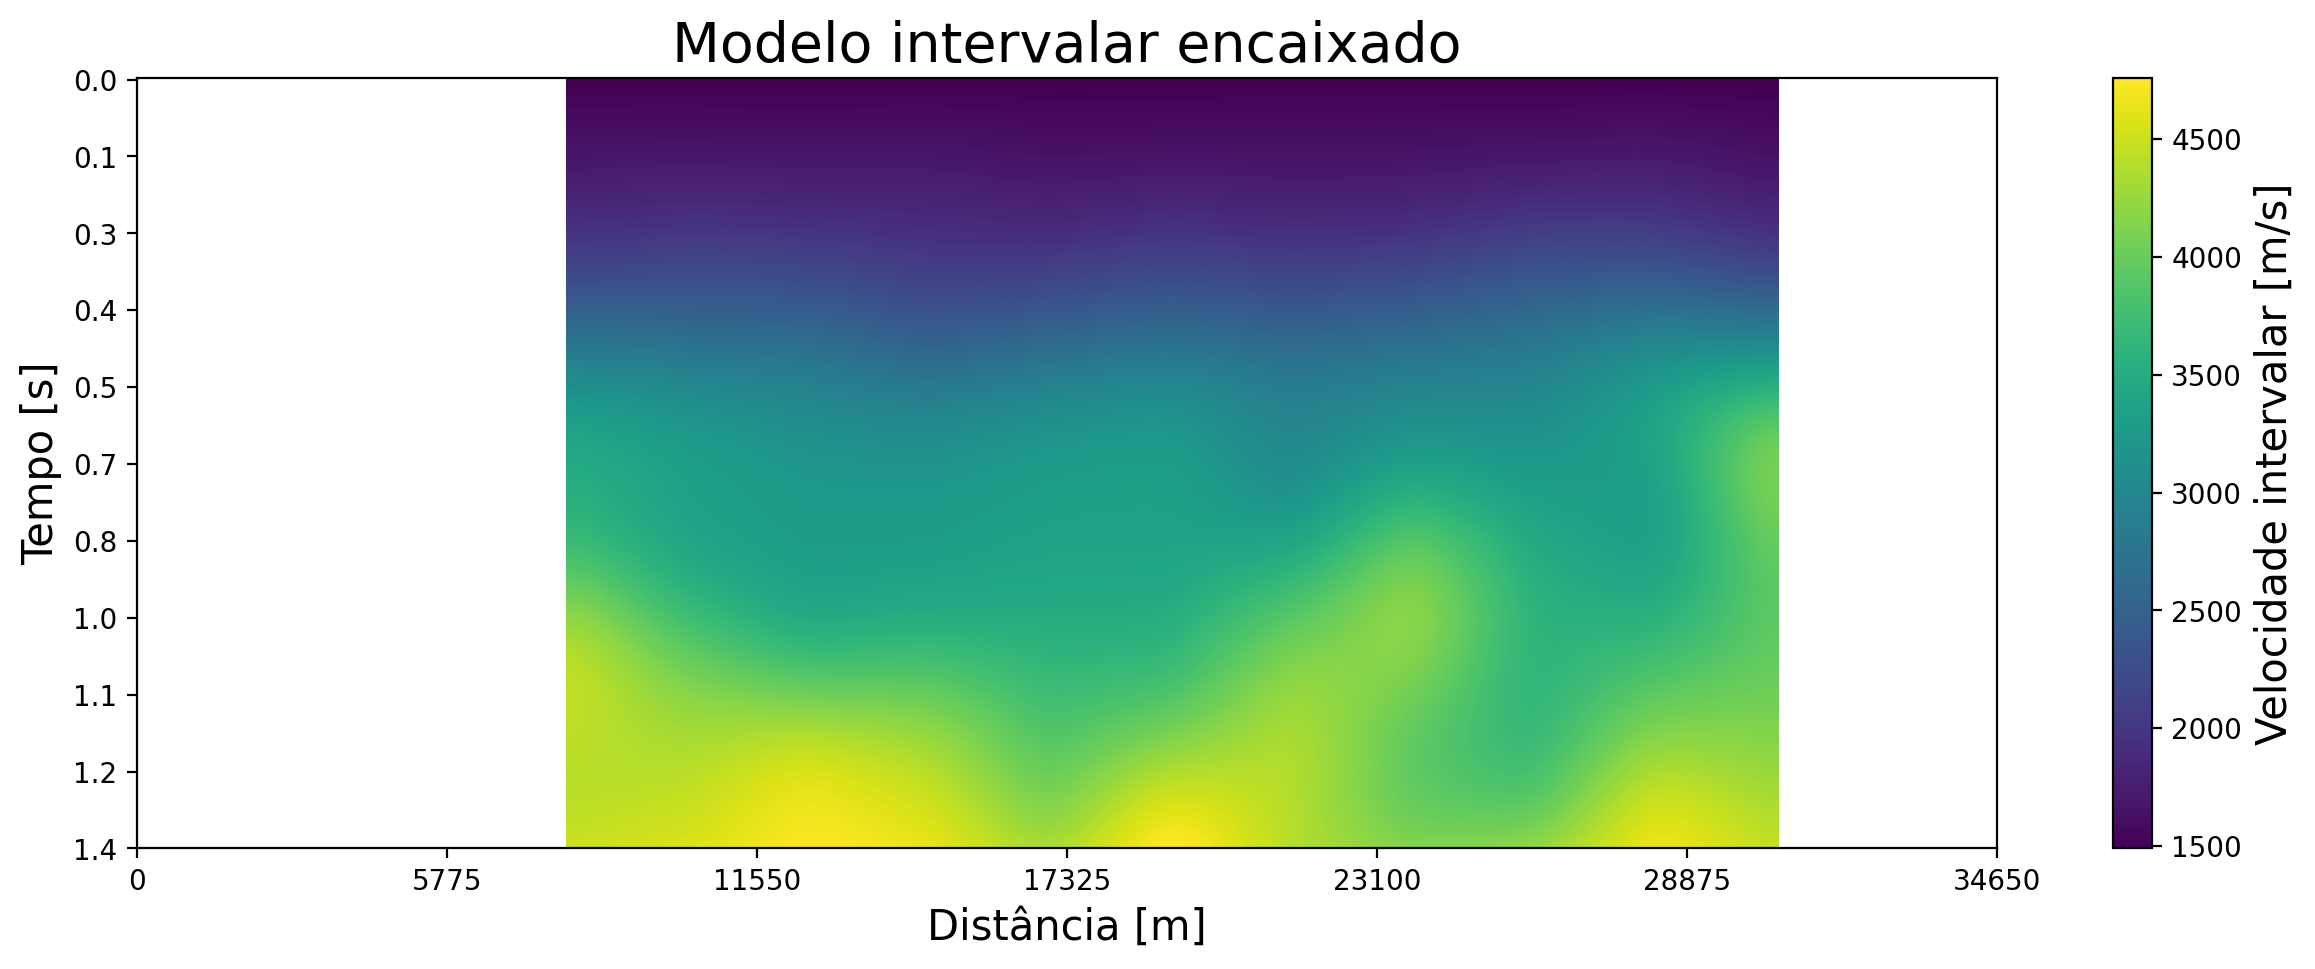
\includegraphics[width=11cm,height=5cm]{../imagens/modeloReduzidoINT.png}	
				\tiny{\caption{Modelo estimado somente com dados dos CMPs completos encaixados na geometria de aquisição.}} 	
			\end{figure}			
		\end{column}
	\end{columns}	
	
\end{frame}
% ----------------- NOVO SLIDE --------------------------------	
\begin{frame}{Construção do modelo de velocidades $v_p$}
	\framesubtitle{Extrapolação lateral do modelo $v_p$}	
	
	\begin{columns}[onlytextwidth, T]
		\begin{column}{.9\textwidth}
			\begin{figure}[h]
				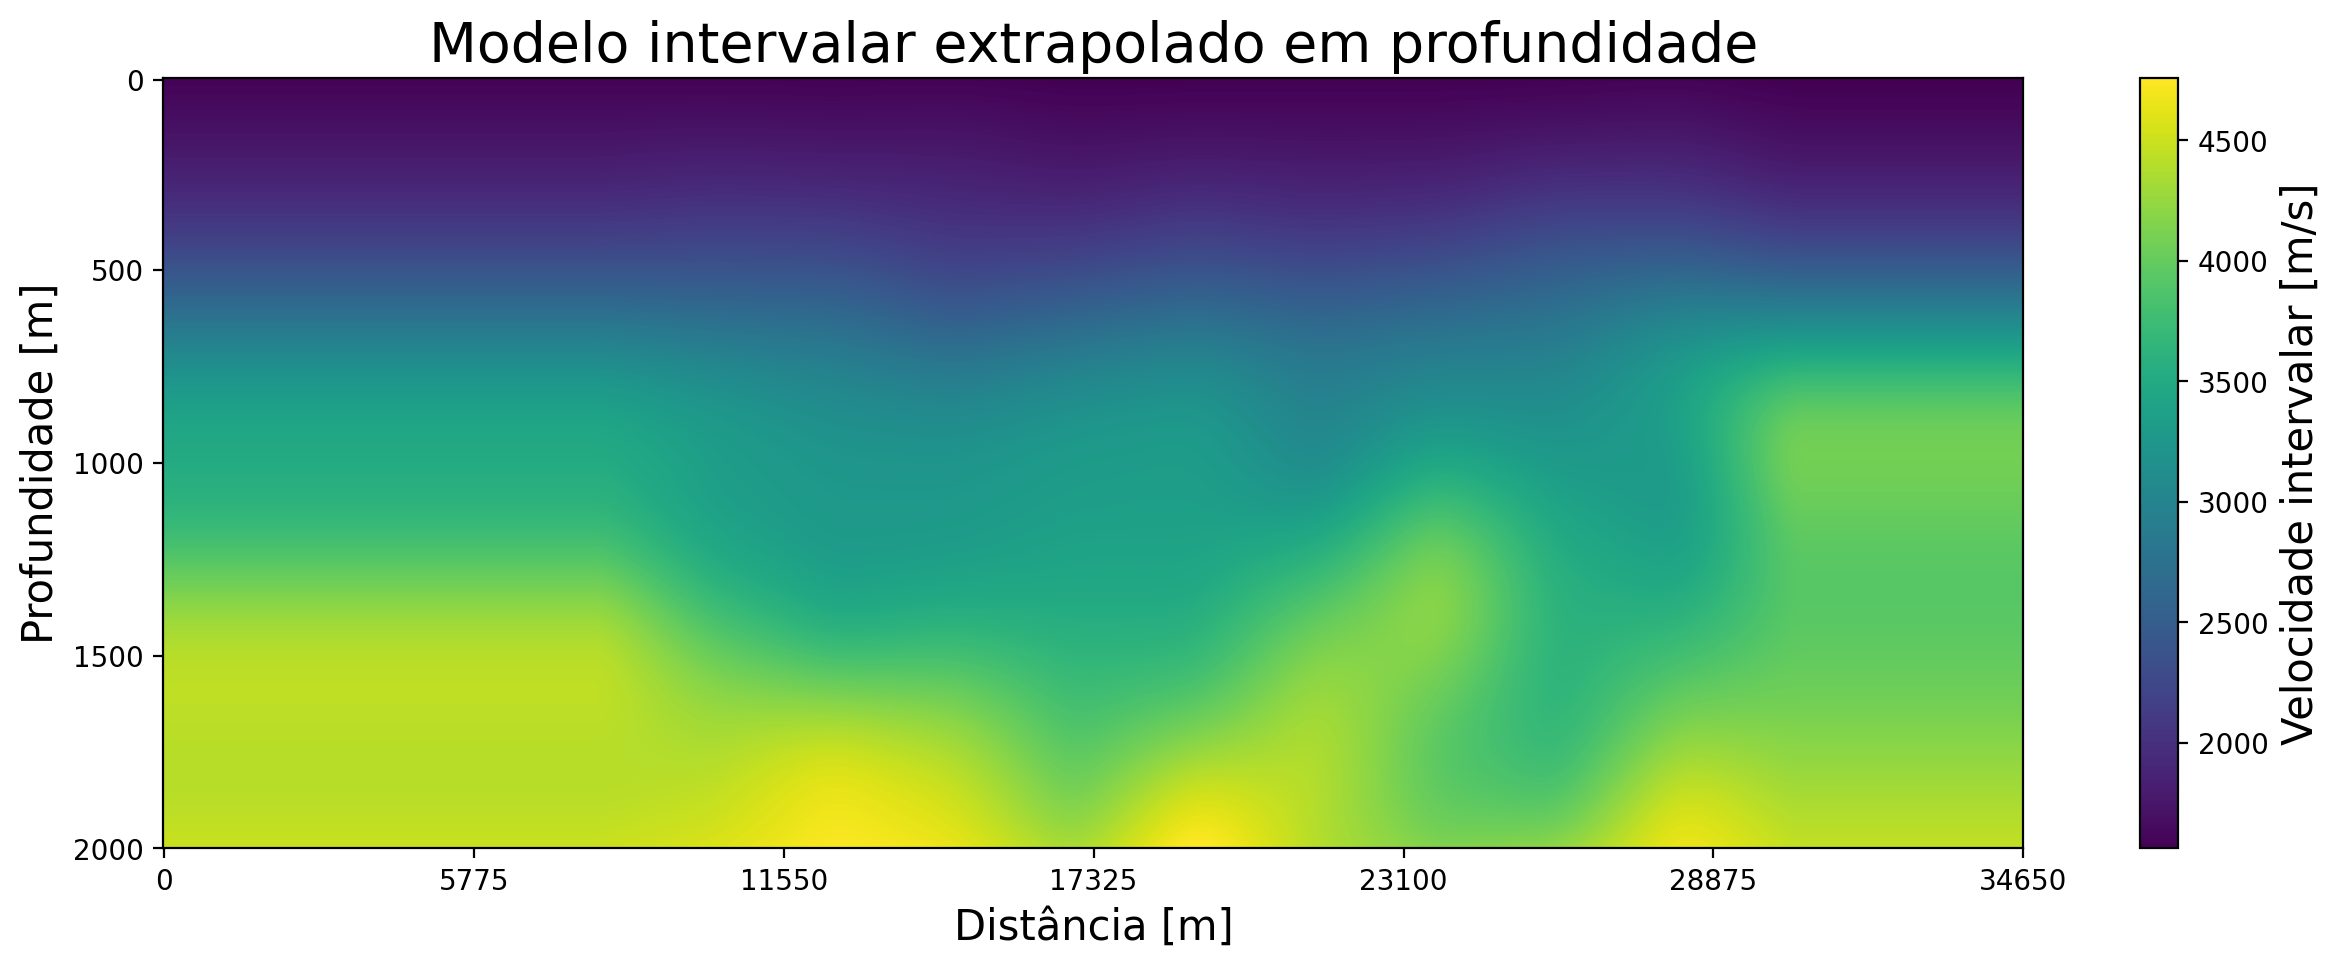
\includegraphics[width=11cm,height=5cm]{../imagens/modeloExtrapoladoINT.png}	
				\tiny{\caption{Modelo $v_p$ completo em profundidade.}} 	 	
			\end{figure}			
			\begin{itemize}
				\small
				\item[$\bullet$] nx = 2772 amostras; $\,\,\,\,$ dx = 12,5 m
				\item[$\bullet$] nz = 323 amostras; $\,\,\,\,\,\,\,$ dz = 6,192 m	
			\end{itemize}
		\end{column}
	\end{columns}	
	
\end{frame}
% ----------------- NOVO SLIDE --------------------------------	
\begin{frame}{Empilhamento do dado real}
\framesubtitle{Seção empilhada e migrada em tempo utilizando a migração \citeonline{stolt1978migration}}	

\pause	
\begin{columns}[onlytextwidth, T]
	\begin{column}{.9\textwidth}
		\begin{figure}[h]
			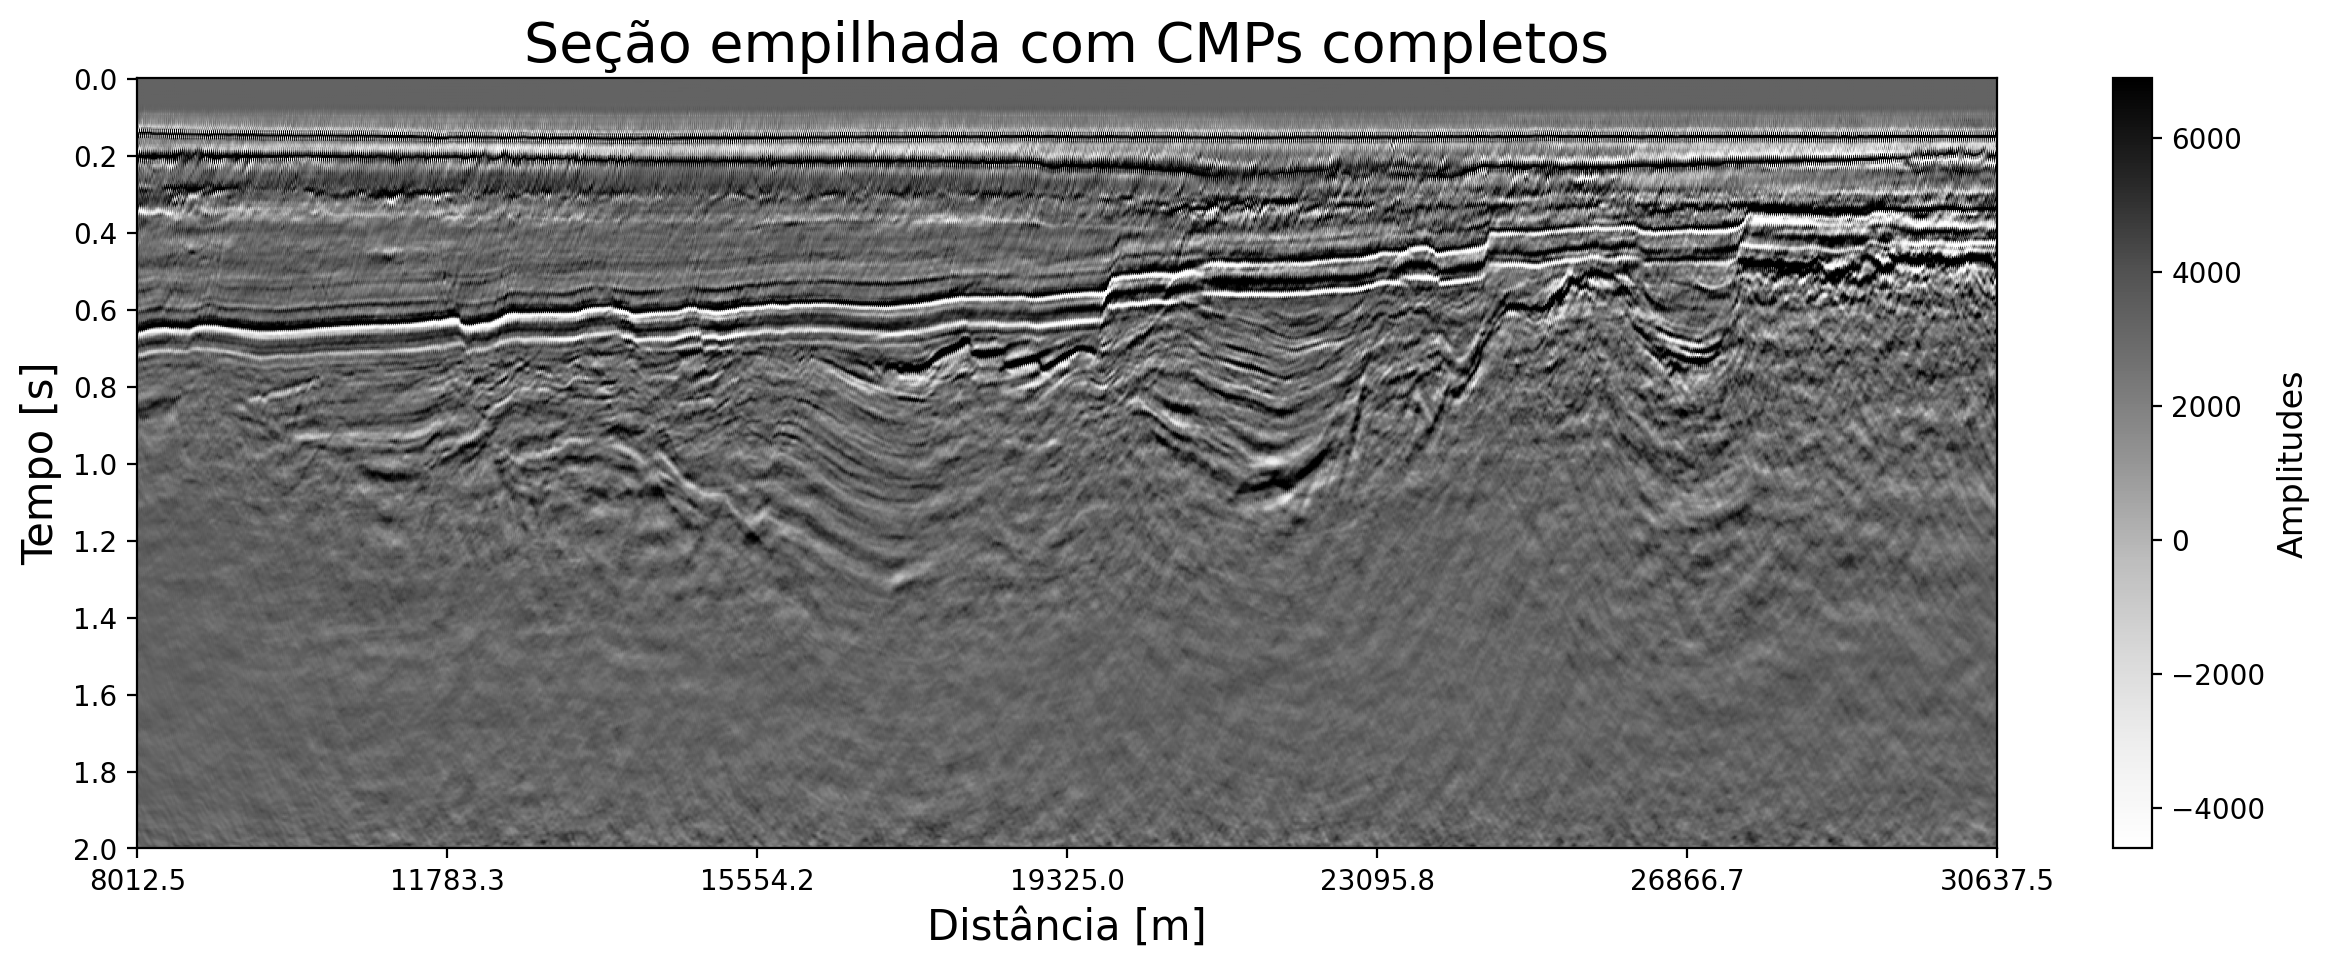
\includegraphics[width=11cm,height=5cm]{../imagens/section.png}	
			\tiny{\caption{Seção empilhada e migrada em tempo projetada nos CMPs de varredura completa, resultado base para as comparações.}} 	
		\end{figure}			
	\end{column}
\end{columns}	
		
\end{frame}
% ----------------- NOVO SLIDE --------------------------------	
\begin{frame}{Construção dos modelos de propriedades elásticas}
	\framesubtitle{Coleta de horizontes da seção empilhada}	
	
	\pause	
	\begin{columns}[onlytextwidth, T]
		\begin{column}{.9\textwidth}
			\begin{figure}[h]
				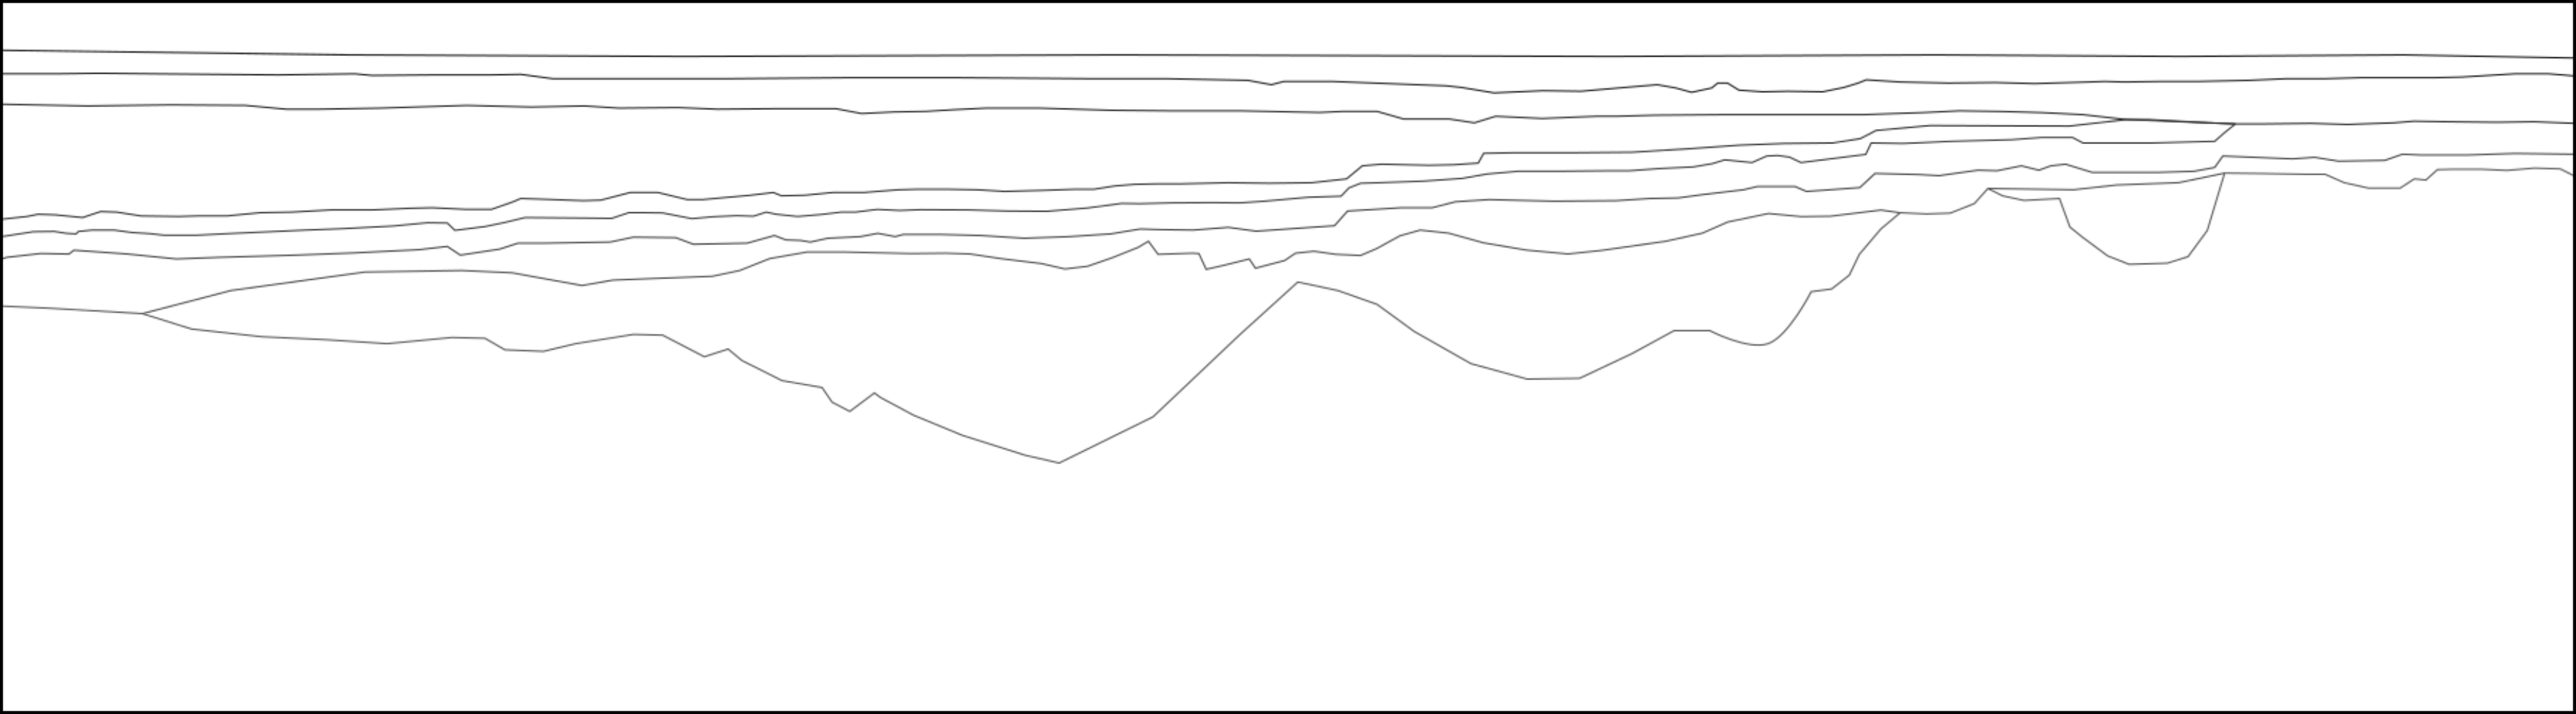
\includegraphics[width=11cm,height=5cm]{../imagens/horizontes.png}	
				\tiny{\caption{Horizontes interpretados a partir da seção empilhada e migrada. Programa \textit{Inkscape} utilizado para contornar os horizontes na mesma dimensão da seção sísmica.}} 	
			\end{figure}			
		\end{column}
	\end{columns}	
	
\end{frame}
% ----------------- NOVO SLIDE --------------------------------	
\begin{frame}{Construção dos modelos de propriedades elásticas}
	\framesubtitle{Importação dos horizontes e conversão da imagem para matriz de posições}	
		
	\begin{columns}[onlytextwidth, T]
		\begin{column}{.9\textwidth}
			\begin{figure}[h]
				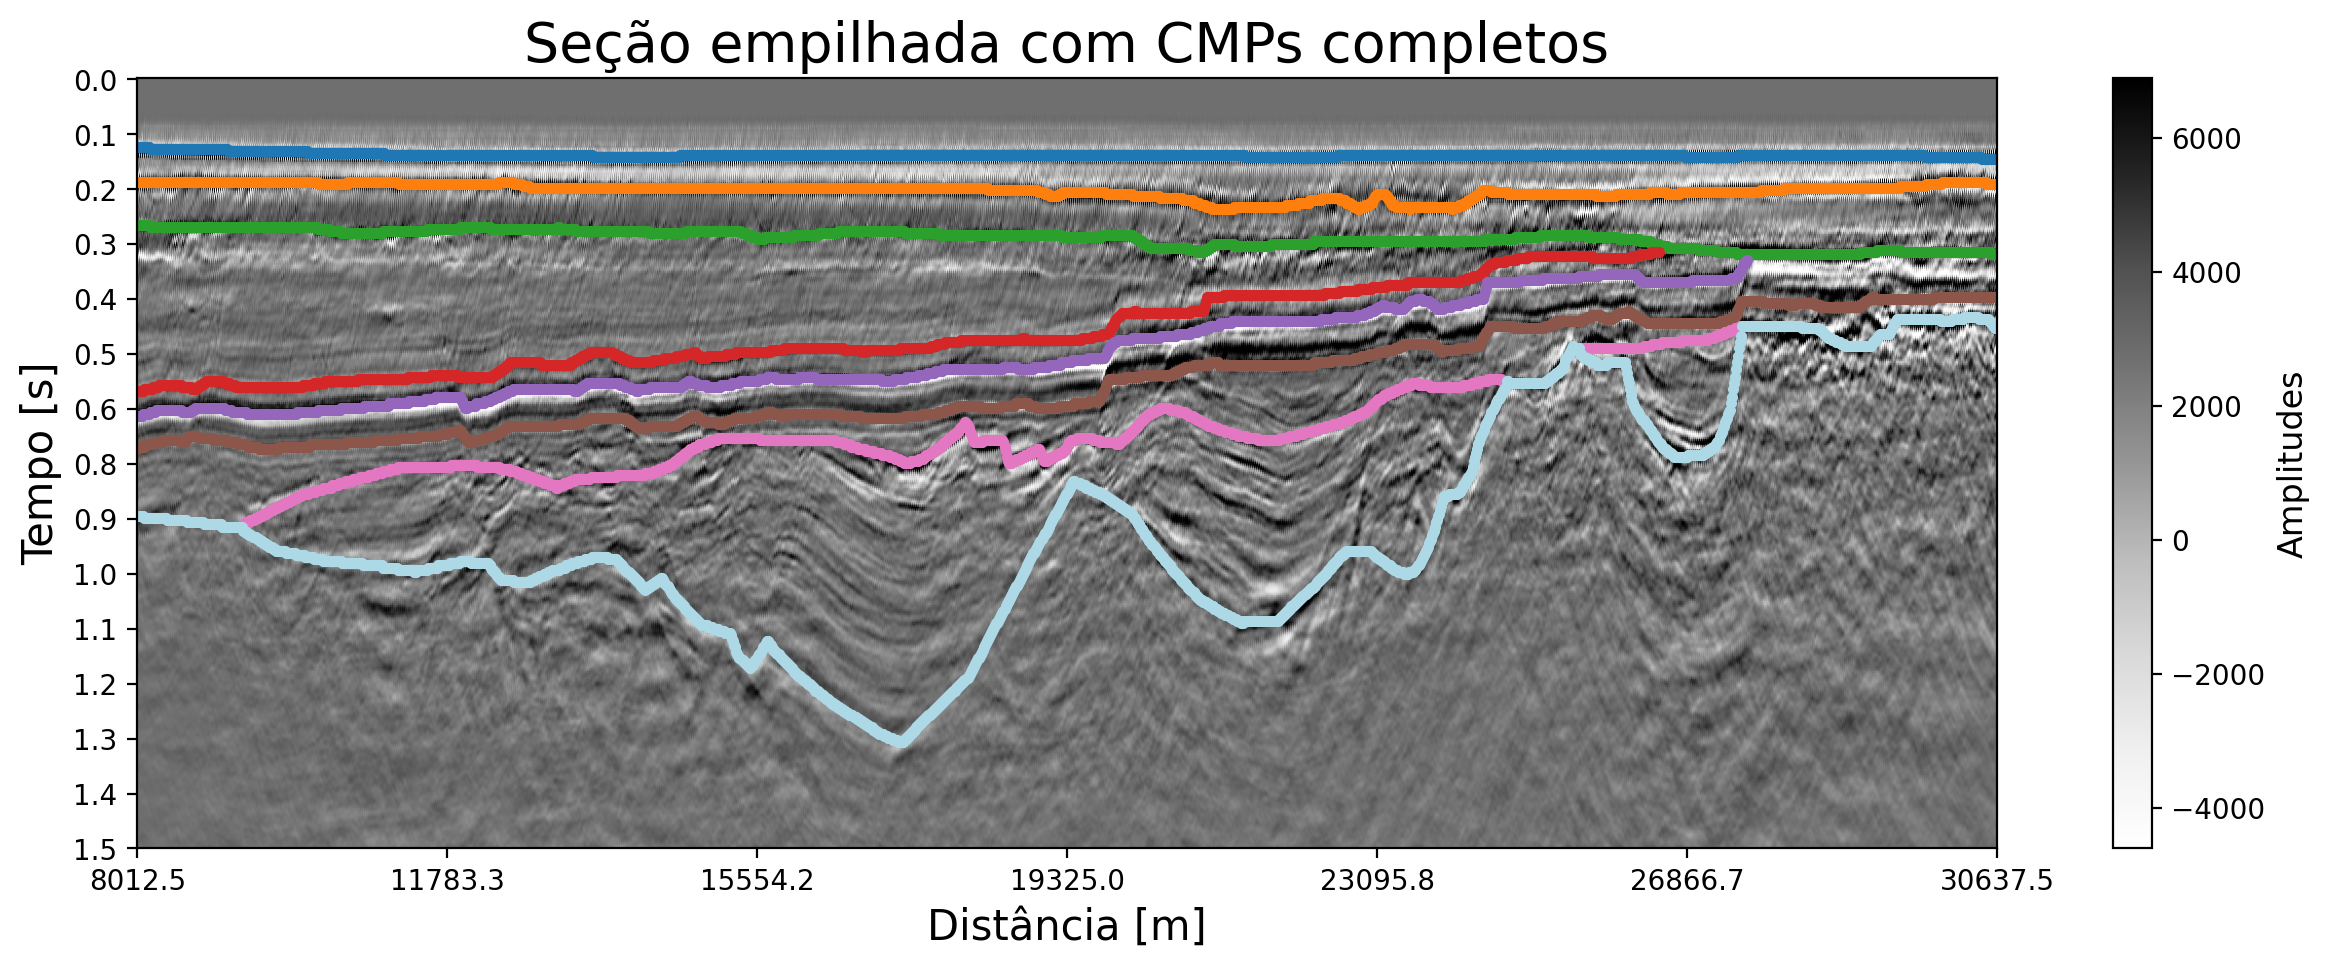
\includegraphics[width=11cm,height=5cm]{../imagens/sectionHrz.png}	
				\tiny{\caption{Projeção dos horizontes na seção empilhada e migrada em tempo.}} 	
			\end{figure}			
		\end{column}
	\end{columns}	
	
\end{frame}
% ----------------- NOVO SLIDE --------------------------------	
\begin{frame}{Construção dos modelos de propriedades elásticas}
	\framesubtitle{Construção do modelo abrupto contendo as velocidades médias $v_p$}	
		
	\begin{columns}[onlytextwidth, T]
		\begin{column}{.9\textwidth}
			\begin{figure}[h]
				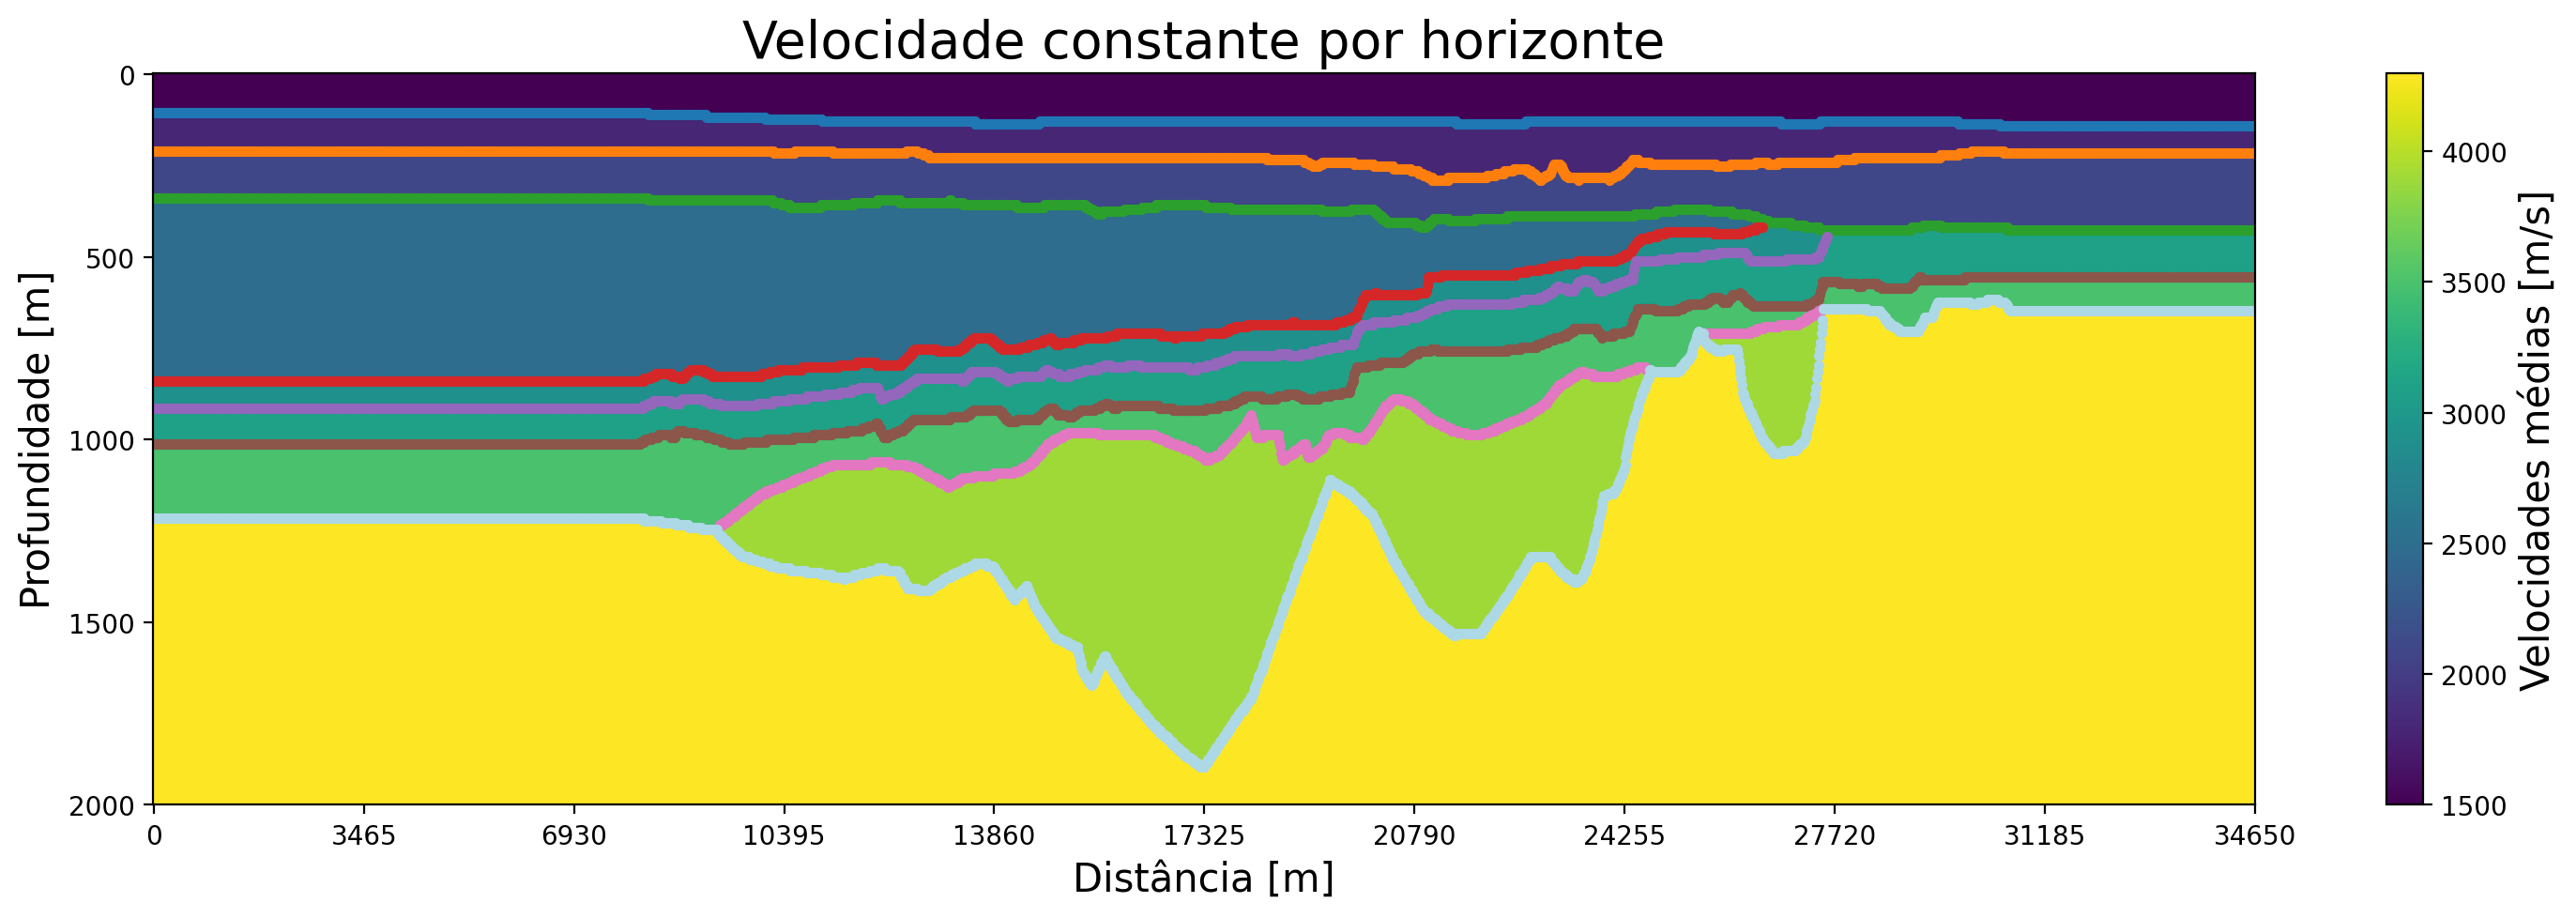
\includegraphics[width=11cm,height=5cm]{../imagens/modeloAbrupto.png}	
				\tiny{\caption{Modelo $v_p$ gerado a partir dos horizontes para estimar as propriedades elásticas $v_s$ e $\rho$.}} 	
			\end{figure}			
		\end{column}
	\end{columns}	
	
\end{frame}
% ----------------- NOVO SLIDE --------------------------------	
\begin{frame}{Construção dos modelos de propriedades elásticas}
	\framesubtitle{Modelos de $v_{INT}$, $v_s$ e $\rho$ gerados para realizar a modelagem de propagação de ondas}	
	
	\begin{columns}[onlytextwidth, T]
		\begin{column}{.6\textwidth}
			\begin{figure}[h]
				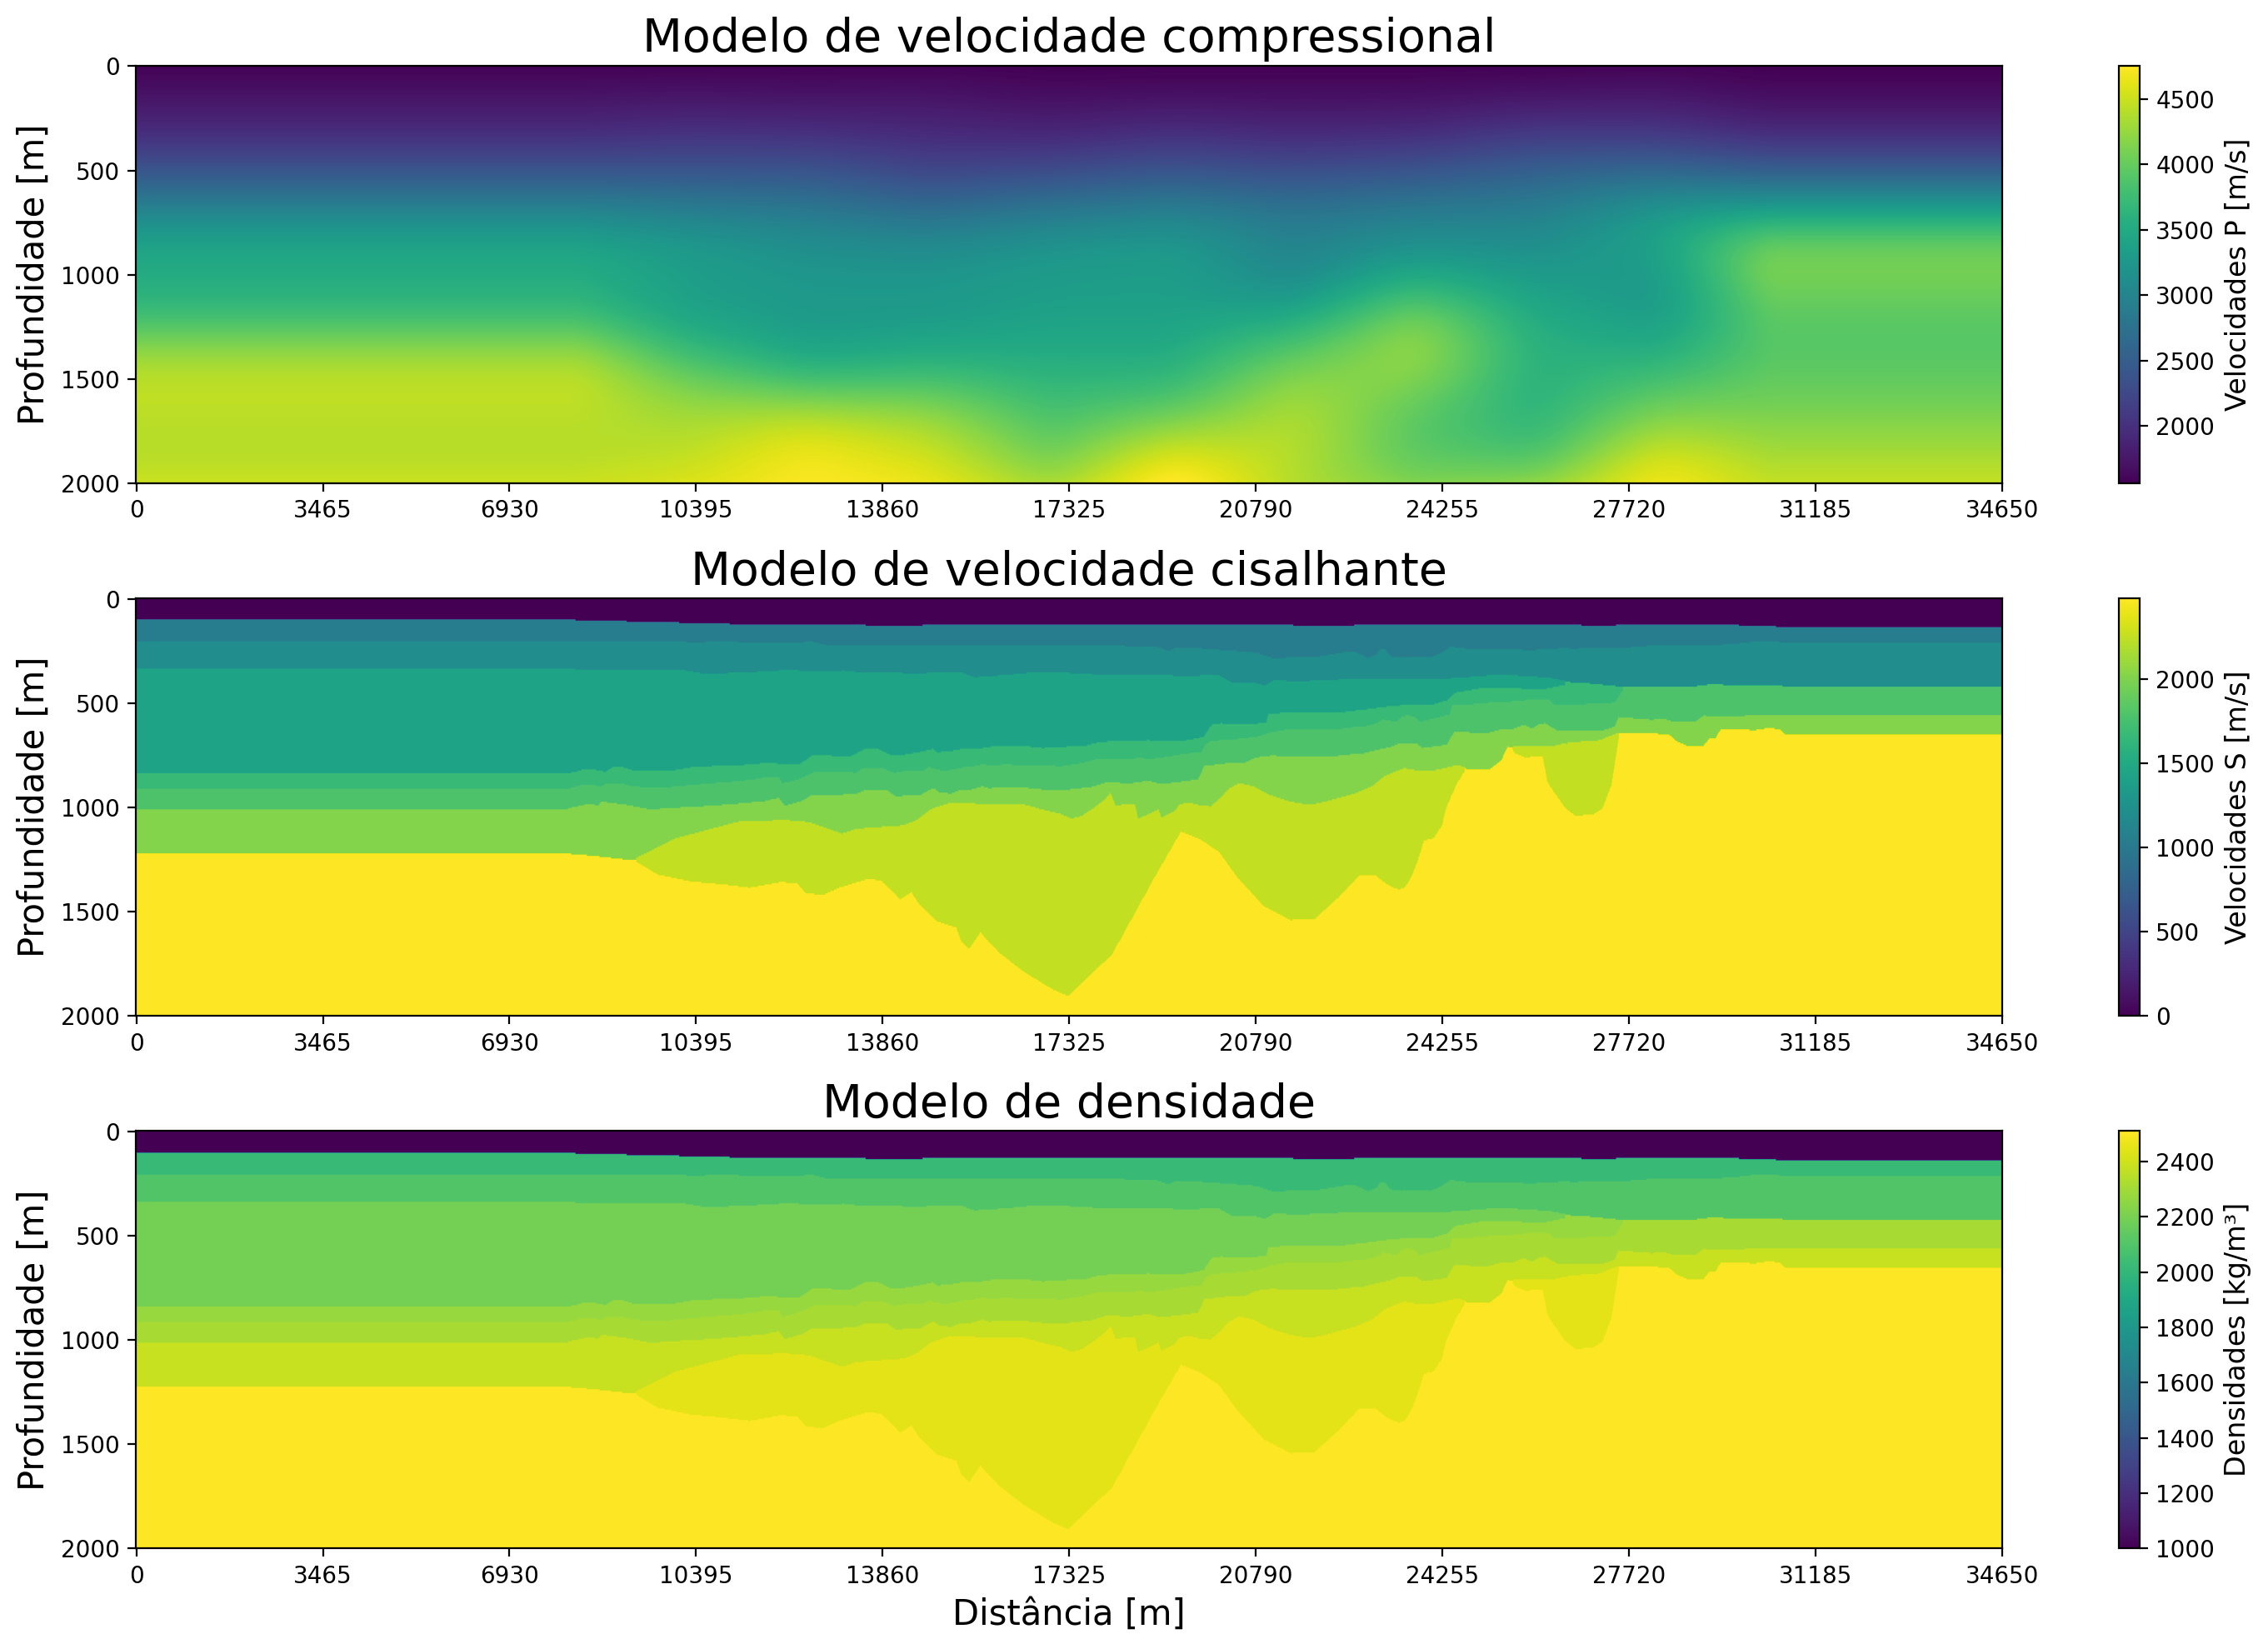
\includegraphics[width=8cm,height=6cm]{../imagens/ModelosInput.png}	
				\tiny{\caption{Modelos utilizados para a propagação da onda em meio elástico.}} 	
			\end{figure}			
		\end{column}
	
		\begin{column}{.35\textwidth}
			\begin{itemize}
				\small\bigskip\bigskip\bigskip 
				\item[$\bullet$] $v_{INT}$ \newline  \text{\scriptsize Modelo estimado VelAn}
				
				\bigskip\bigskip\bigskip
				\item[$\bullet$] $v_s \approx v_p / 1,7$\newline \text{\scriptsize Kearey (2013)}
				
				\bigskip\bigskip
				\item[$\bullet$] $\rho \approx 310 \,v_p^{0,25}$\newline \text{\scriptsize Gardner (1974)}
			\end{itemize}	
		\end{column}
	\end{columns}	
 \end{frame}
% ----------------- NOVO SLIDE --------------------------------	
\begin{frame}{Simulação da aquisição sísmica}
\framesubtitle{Parâmetros utilizados na modelagem sísmica da aquisição}	

\pause
\begin{columns}[onlytextwidth, T]
	\begin{column}{.5\textwidth}
		\begin{itemize}
			\small
			\item[$\to$] Geometria: \textit{End On}
			\item[$\bullet$] 1064 estações de tiros
			\item[$\bullet$] 320 receptores ativos por tiro
		\end{itemize}
		
		\bigskip	
		\begin{itemize}
			\small
			\item[$\to$] \textbf{Tempo:}
			\item[$\bullet$] 3000 amostras
			\item[$\bullet$] 0.5 $ms$ de discretização
			\item[$\bullet$] 1,5 $s$ de tempo total
		\end{itemize}
		
		\bigskip
		\begin{itemize}
			\small
			\item[$\to$] \textbf{Armazenamento:}
			\item[$\bullet$] 4,1 GB de ocupação em disco
		\end{itemize}		
	\end{column}
	
	\begin{column}{.5\textwidth}
		\begin{itemize}
			\small
			\item[$\to$] Espaço:
			\item[$\bullet$] 100 m de \textit{offset} mínimo
			\item[$\bullet$] 8 km de \textit{spread}		
			\item[$\bullet$] 25 m entre receptores
			\item[$\bullet$] 25 m entre fontes
			\item[$\bullet$] 22650 m de cobertura sísmica
			\item[$\bullet$] 34650 m de aquisição sísmica
		\end{itemize}		
		
		\bigskip
		\begin{itemize}
			\small
			\item[$\to$] \textbf{Modelo:}
			\item[$\bullet$] 5544 amostras na horizontal
			\item[$\bullet$] 323 amostras na vertical
			\item[$\bullet$] 6,25 m discretização x 
			\item[$\bullet$] 6,192 m discretização z			
		\end{itemize}
	\end{column}
\end{columns}

\end{frame}
% ----------------- NOVO SLIDE --------------------------------	
\begin{frame}{Simulação da aquisição sísmica}
\framesubtitle{Estimativa da assinatura da fonte sísmica}	
	
\begin{columns}[onlytextwidth, T]
	\begin{column}{.9\textwidth}
		\begin{figure}[h]
			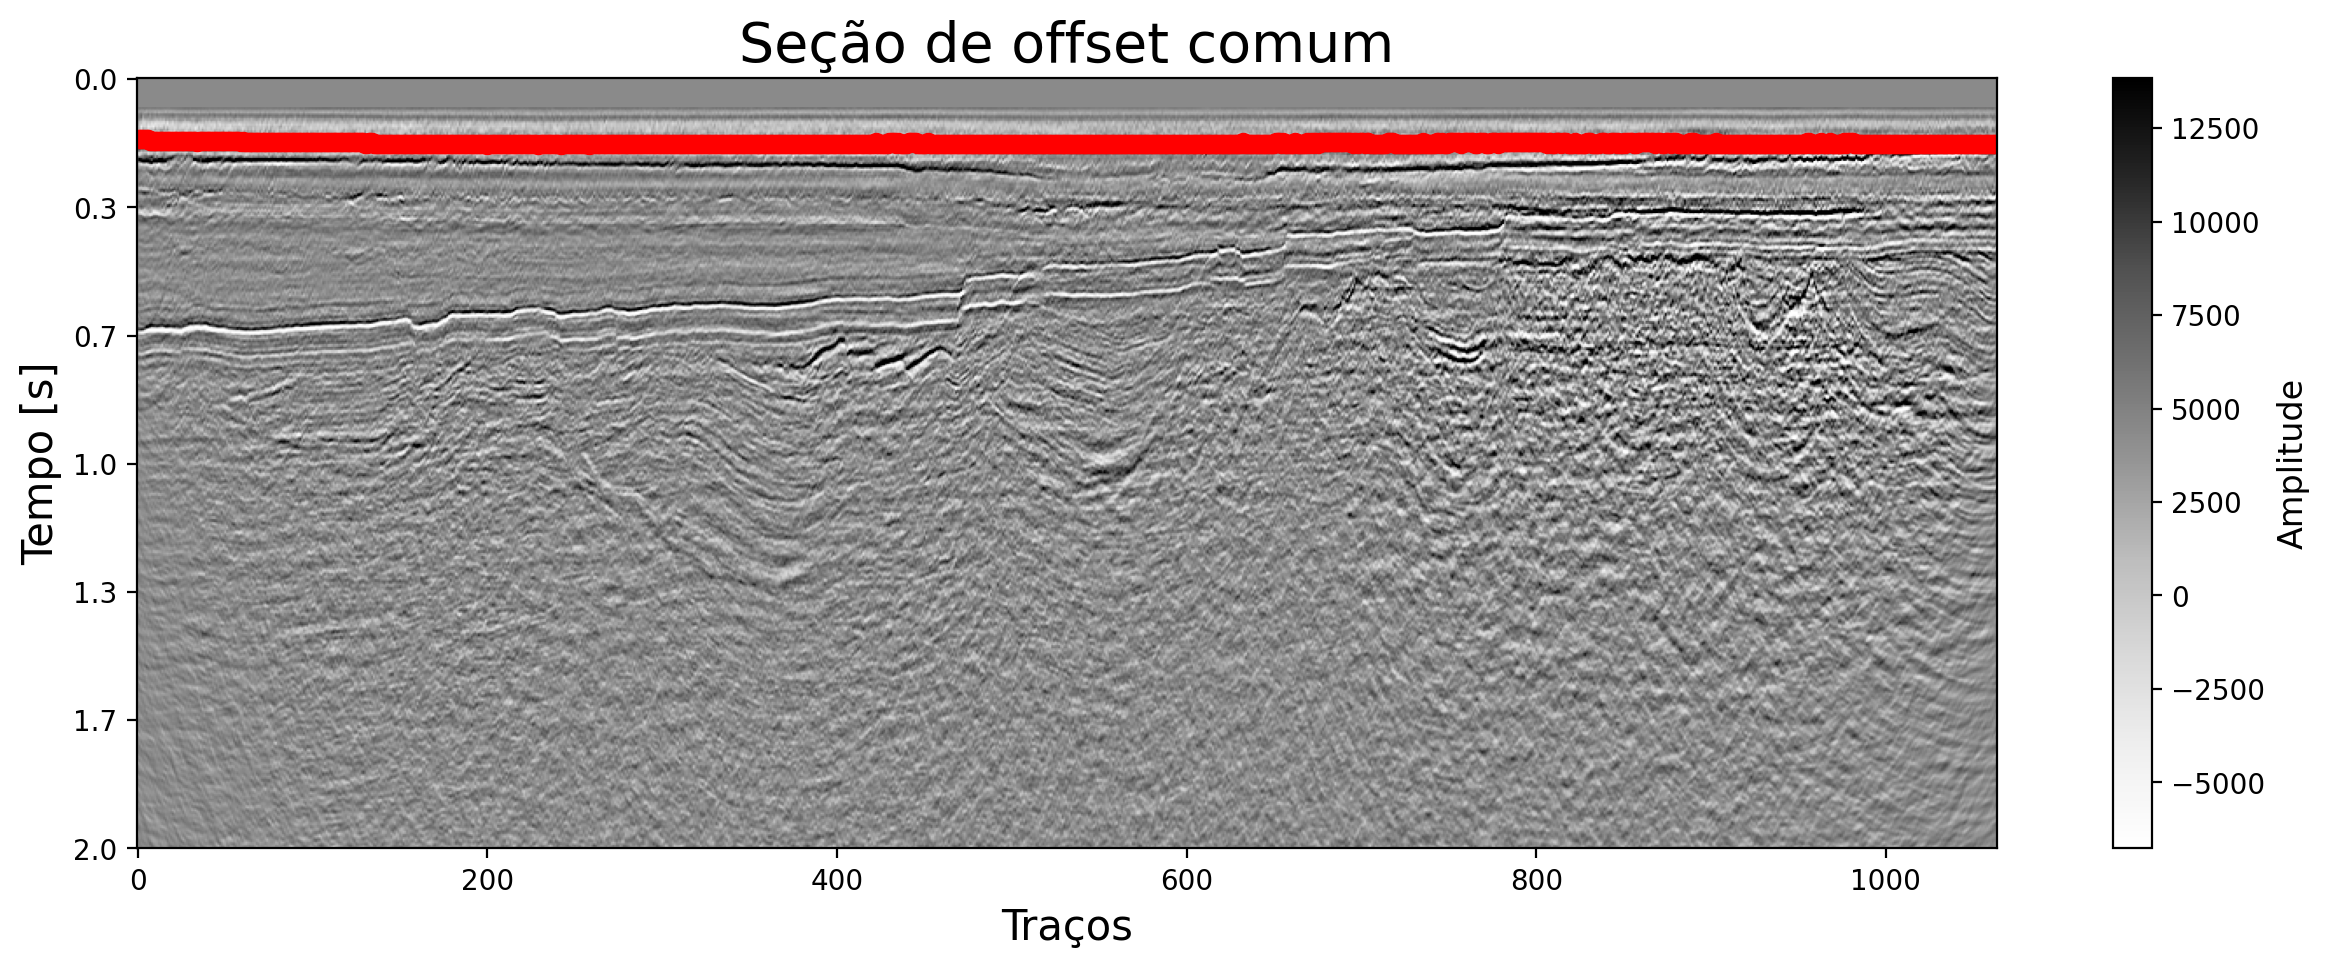
\includegraphics[width=11cm,height=5cm]{../imagens/estimativaWavelet.png}	
			\tiny{\caption{Coleta da reflexão do fundo marinho utilizando a seção de menor \textit{offset}, de 100 metros.}} 	
		\end{figure}			
	\end{column}
\end{columns}	

\end{frame}
% ----------------- NOVO SLIDE --------------------------------	
\begin{frame}{Simulação da aquisição sísmica}
	\framesubtitle{Estimativa da assinatura da fonte sísmica}	
	
	\begin{columns}[onlytextwidth, T]
		\begin{column}{.9\textwidth}
			\begin{figure}[h]
				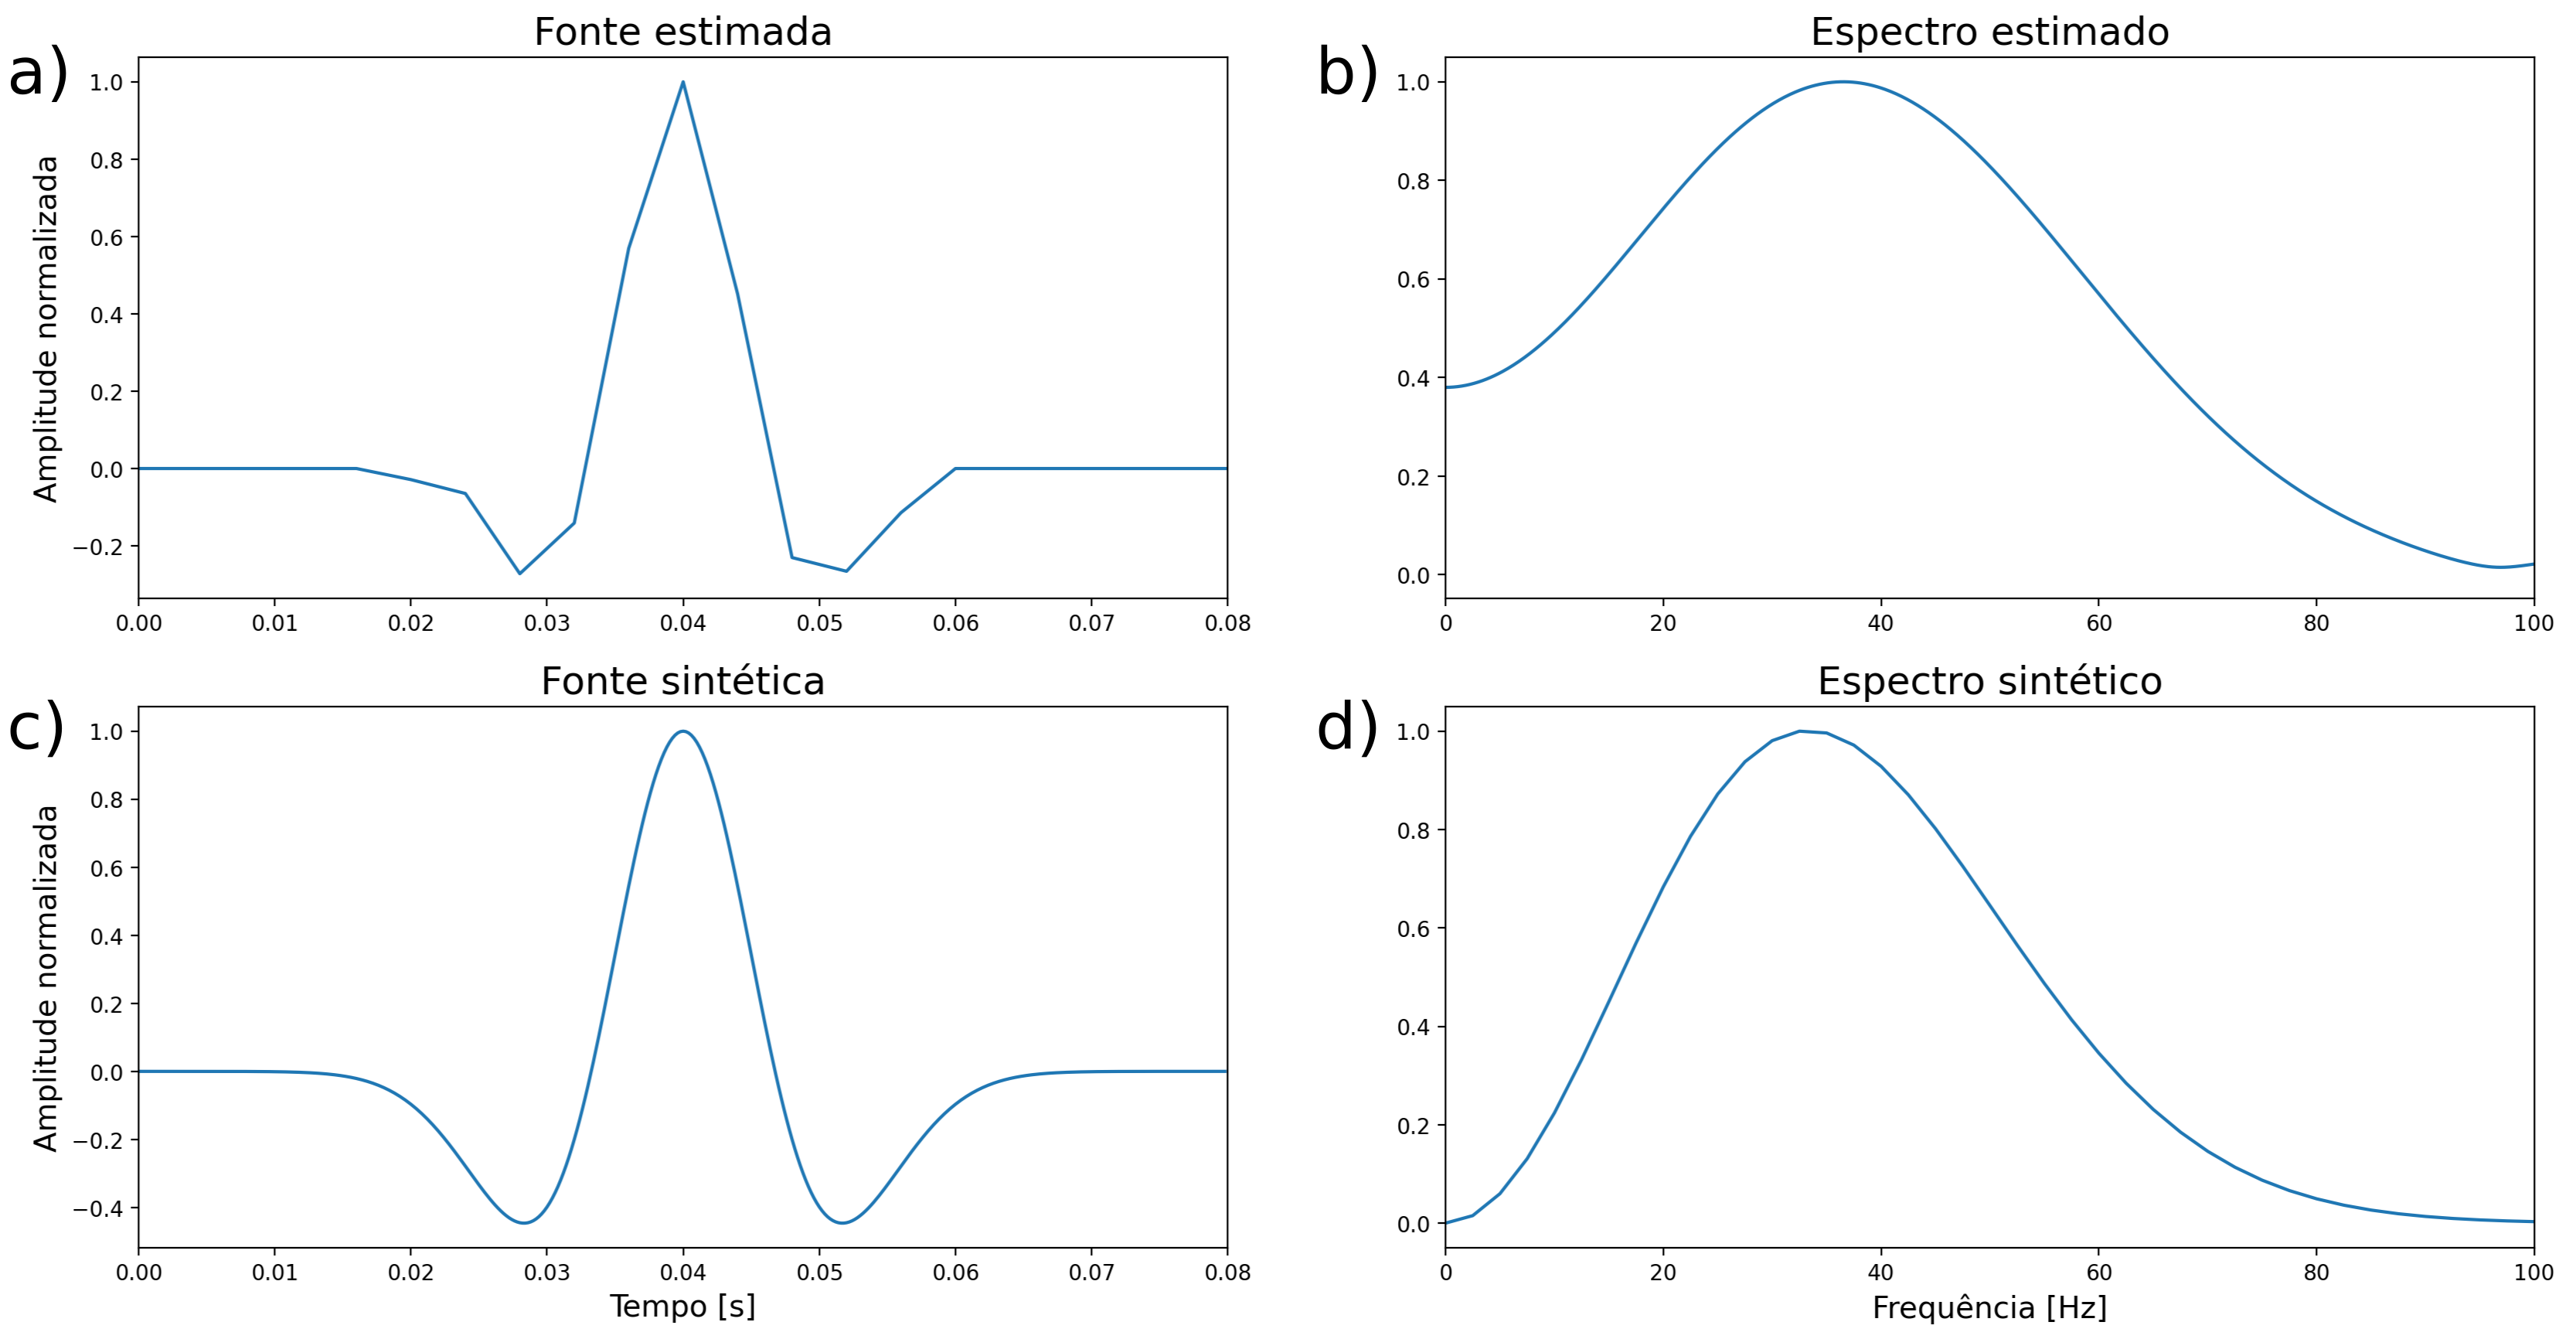
\includegraphics[width=11cm,height=5cm]{../imagens/waveletsModeling.png}	
				\tiny{\caption{Fonte sintética baseada na fonte estimada com frequência máxima de 100 Hz e 400 amostras.}} 	
			\end{figure}			
		\end{column}
	\end{columns}	
	
\end{frame}
% ----------------- NOVO SLIDE --------------------------------	
\begin{frame}{Pré-condicionamento no dado sintético}
\framesubtitle{Sismograma sintético bruto}	
	
	\pause
	\begin{columns}[onlytextwidth, T]
		\begin{column}{.9\textwidth}
			\begin{figure}[h]
				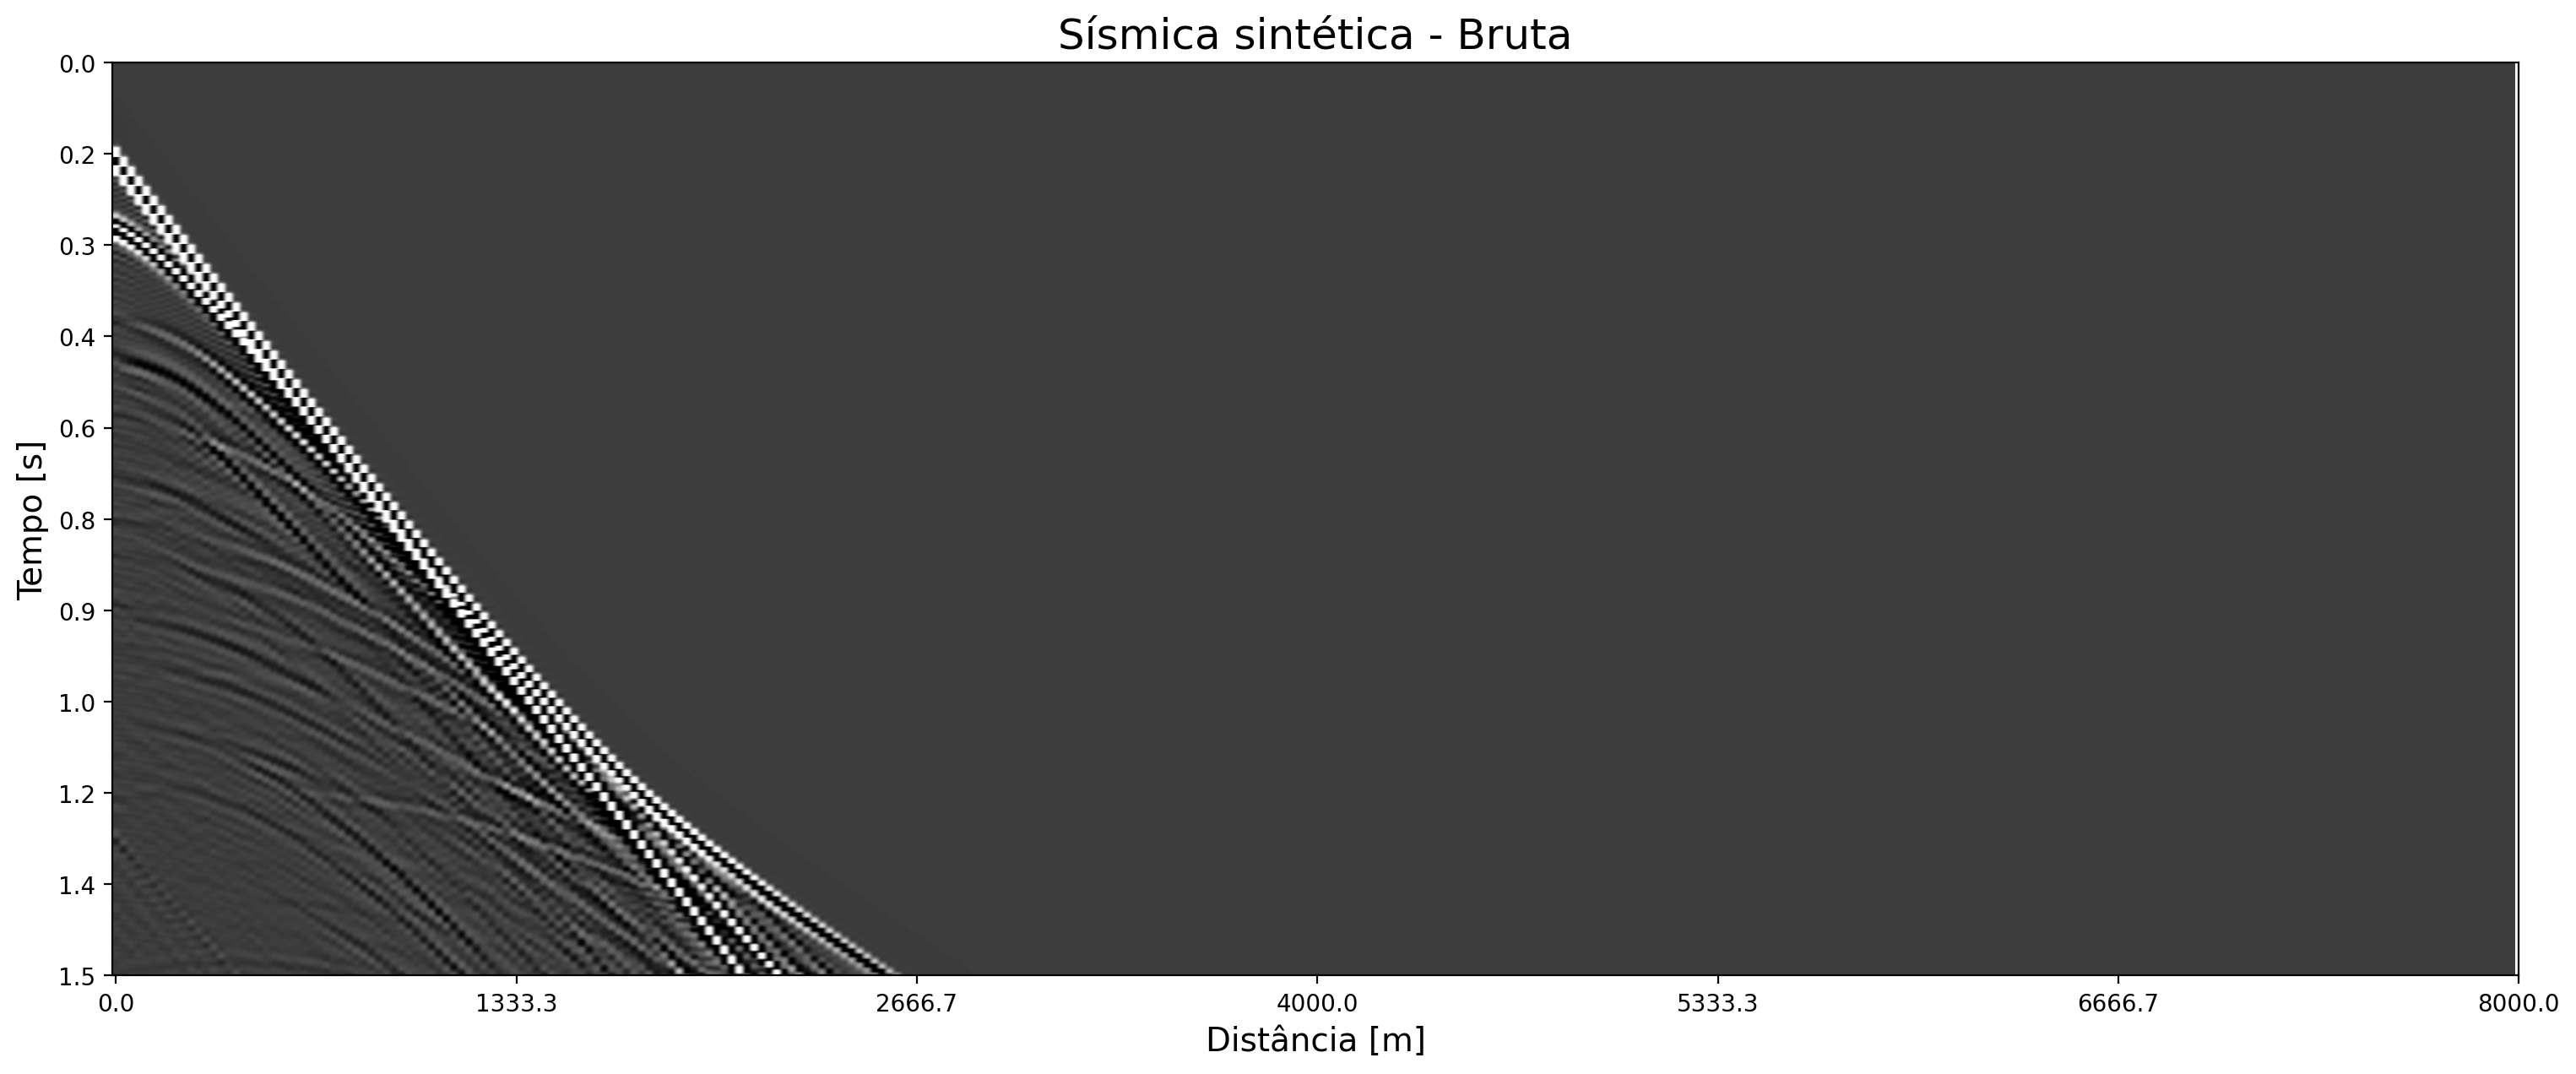
\includegraphics[width=11cm,height=5cm]{../imagens/sismicaSinteticaBruta.png}	
				\tiny{\caption{Onda direta com amplitude alta que atrapalha o empilhamento e corrigir o efeito anti-causal da fonte.}} 	
			\end{figure}			
		\end{column}
	\end{columns}	
	
\end{frame}
% ----------------- NOVO SLIDE --------------------------------	
\begin{frame}{Pré-condicionamento no dado sintético}
	\framesubtitle{Sismograma sintético pré-condicionado}	
	
	\begin{columns}[onlytextwidth, T]
		\begin{column}{.9\textwidth}
			\begin{figure}[h]
				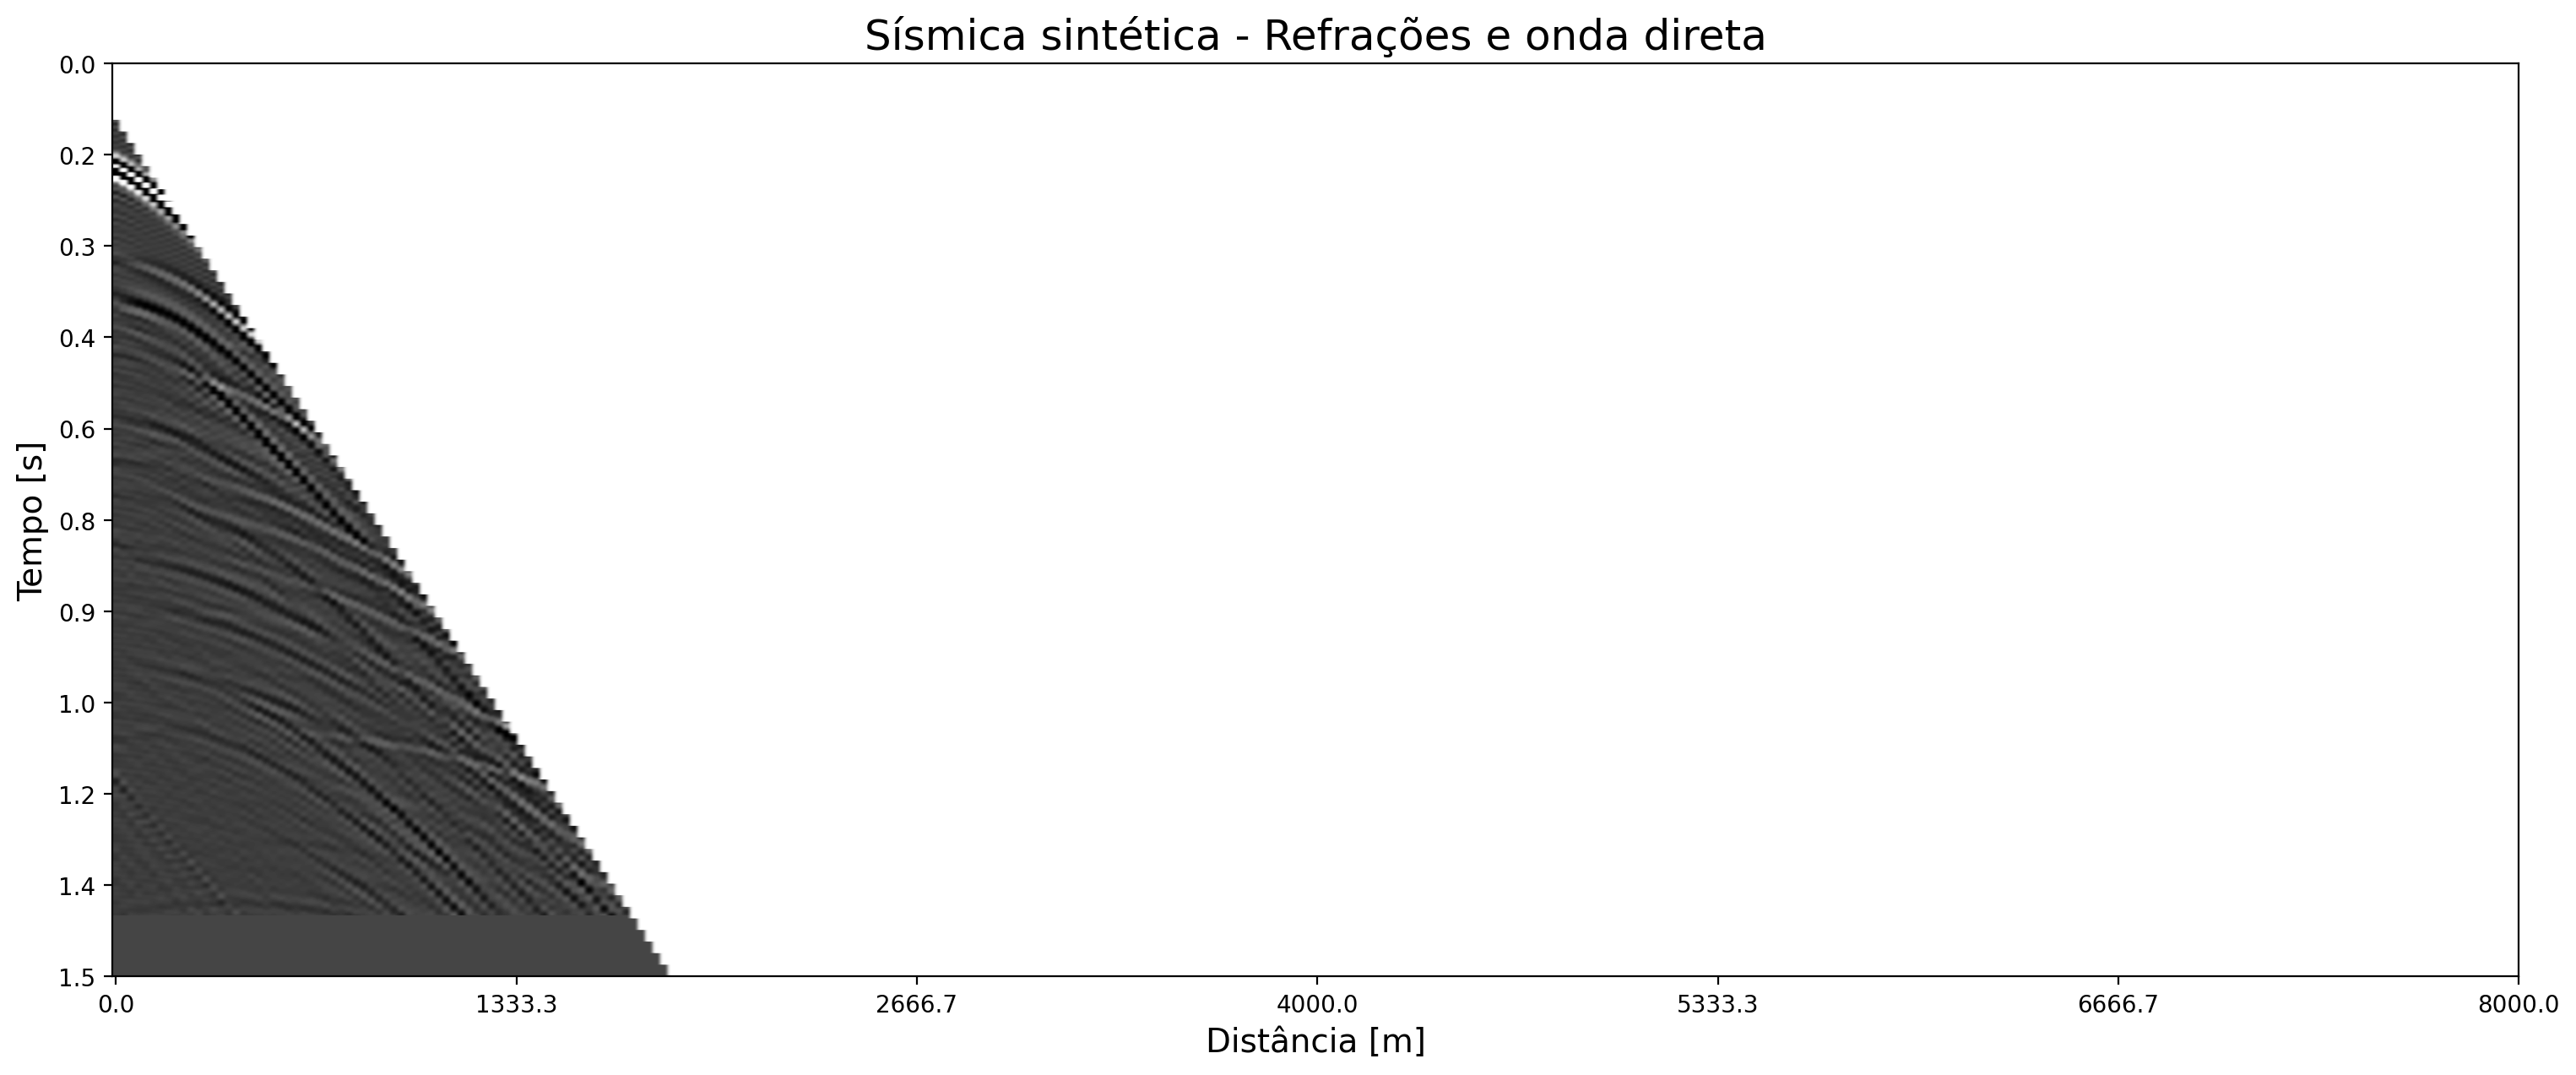
\includegraphics[width=11cm,height=5cm]{../imagens/sismicaMute.png}	
				\tiny{\caption{A onda direta e tempos maiores de 1,4 s foram silenciados.}} 	
			\end{figure}			
		\end{column}
	\end{columns}	
	
\begin{itemize}
	\small
	\item[$\bullet$] Modificações feitas para realizar um novo processo de análise de velocidades e empilhamento.
\end{itemize}		
	
\end{frame}
% ----------------- NOVO SLIDE --------------------------------	
\section{Resultados e discussões}
\begin{frame}{}
	\bigskip\bigskip\bigskip\bigskip\bigskip\bigskip
	\begin{center}
		\Huge Resultados e discussões
	\end{center}    
\end{frame}
% ----------------- NOVO SLIDE --------------------------------	
\begin{frame}{Primeiro resultado obtido}
\framesubtitle{Seções empilhadas e migradas em tempo}	
	
	\begin{columns}[onlytextwidth, T]
		\begin{column}{.9\textwidth}
			\begin{figure}[h]
				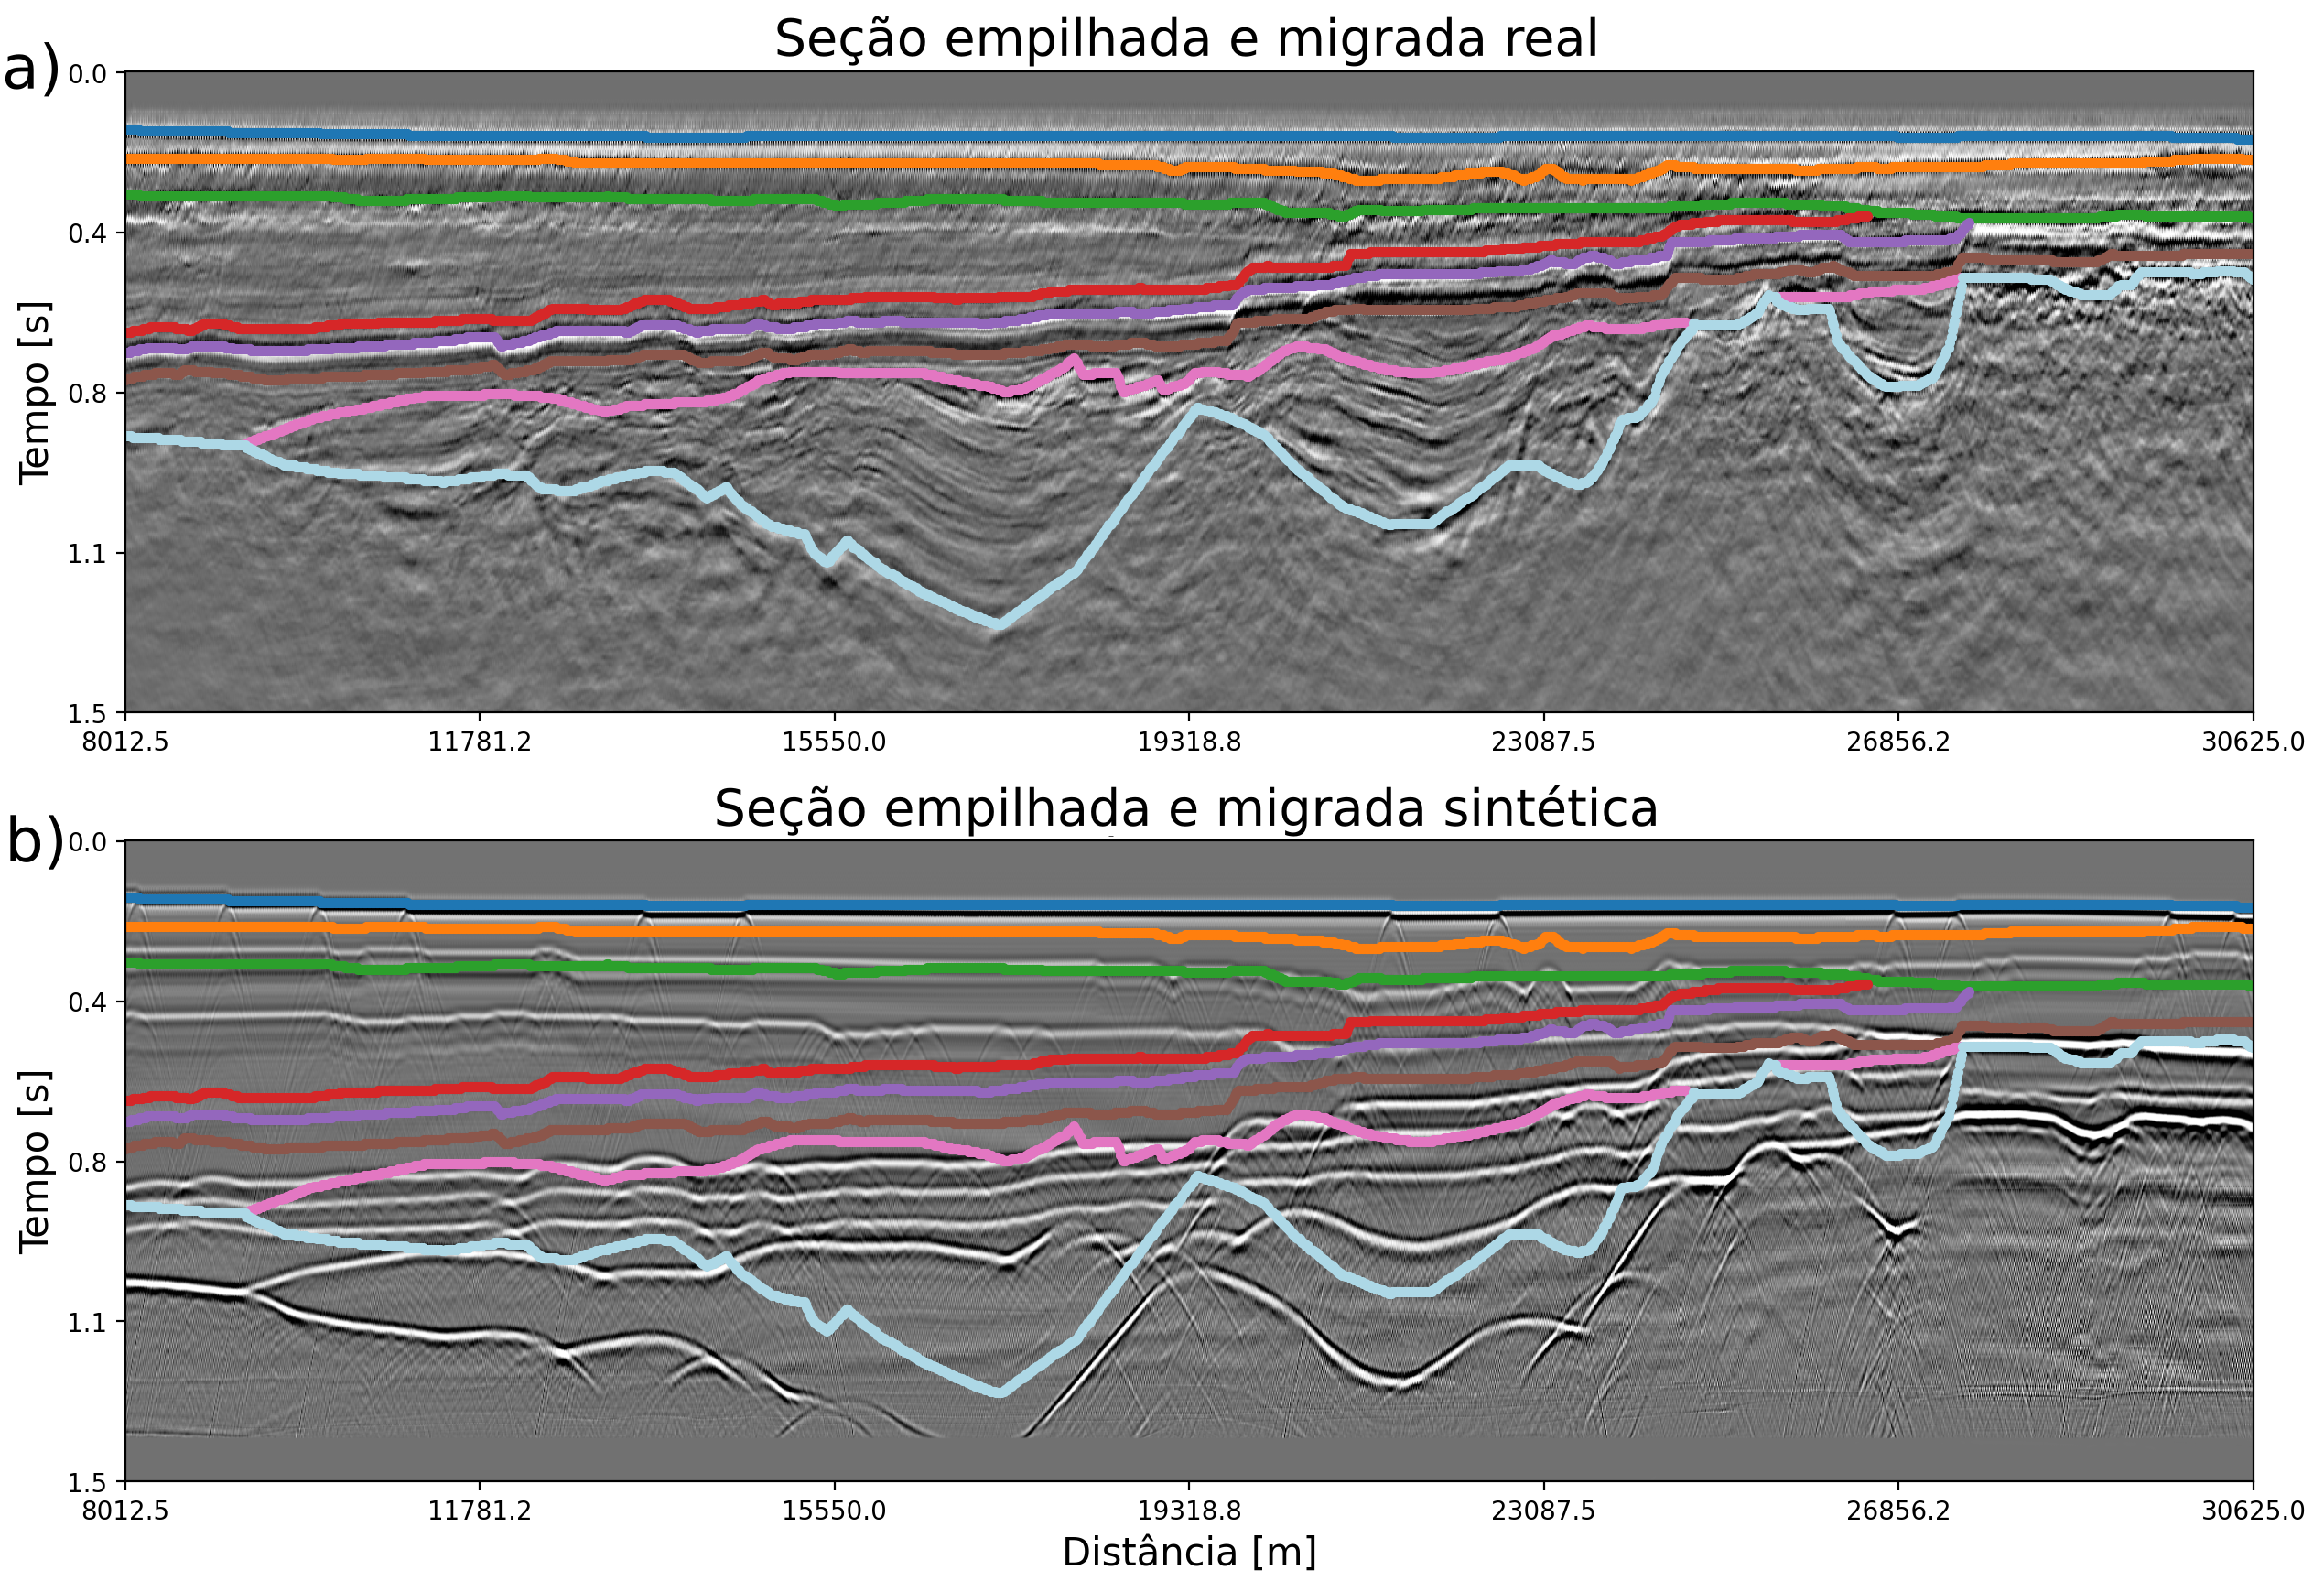
\includegraphics[width=10cm,height=6cm]{../imagens/comparisionHRZ.png}	
				\tiny{\caption{Horizontes coletados do dado real projetados. Detalhe nas reflexões atrasadas no tempo, ou seja, modelo com velocidade baixa.}} 	
			\end{figure}			
		\end{column}
	\end{columns}	
	
\end{frame}
% ----------------- NOVO SLIDE --------------------------------	
\begin{frame}{Análise dos perfis de poços}
\framesubtitle{Trabalho de \citeonline{ruffell1995seismic} mostrando poços próximos da aquisição}	
	
\begin{columns}[onlytextwidth, T]
	\begin{column}{.9\textwidth}
		\begin{figure}[h]
			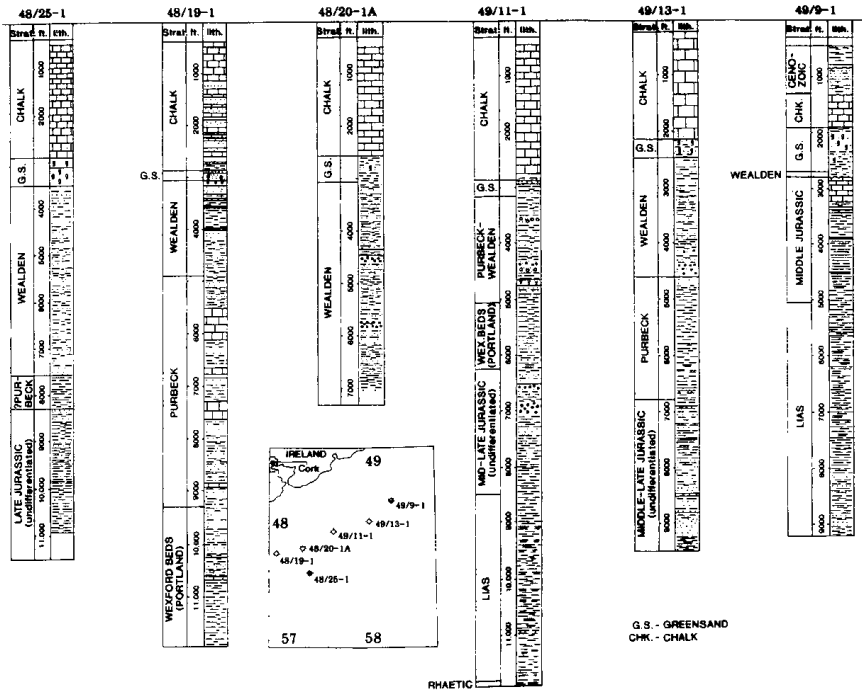
\includegraphics[width=9cm,height=6cm]{../imagens/pocos.png}	
			\tiny{\caption{Poços à direita mais próximos do local de aquisição mostrando a camada rasa de \textit{chalk}.}}
		\end{figure}			
	\end{column}
\end{columns}	
	
\end{frame}
% ----------------- NOVO SLIDE --------------------------------	
\begin{frame}{Atualização do modelo de propriedades}
\framesubtitle{Atualização do modelo de velocidades no tempo}	
	
\begin{columns}[onlytextwidth, T]
	\begin{column}{.9\textwidth}
		\begin{figure}[h]
			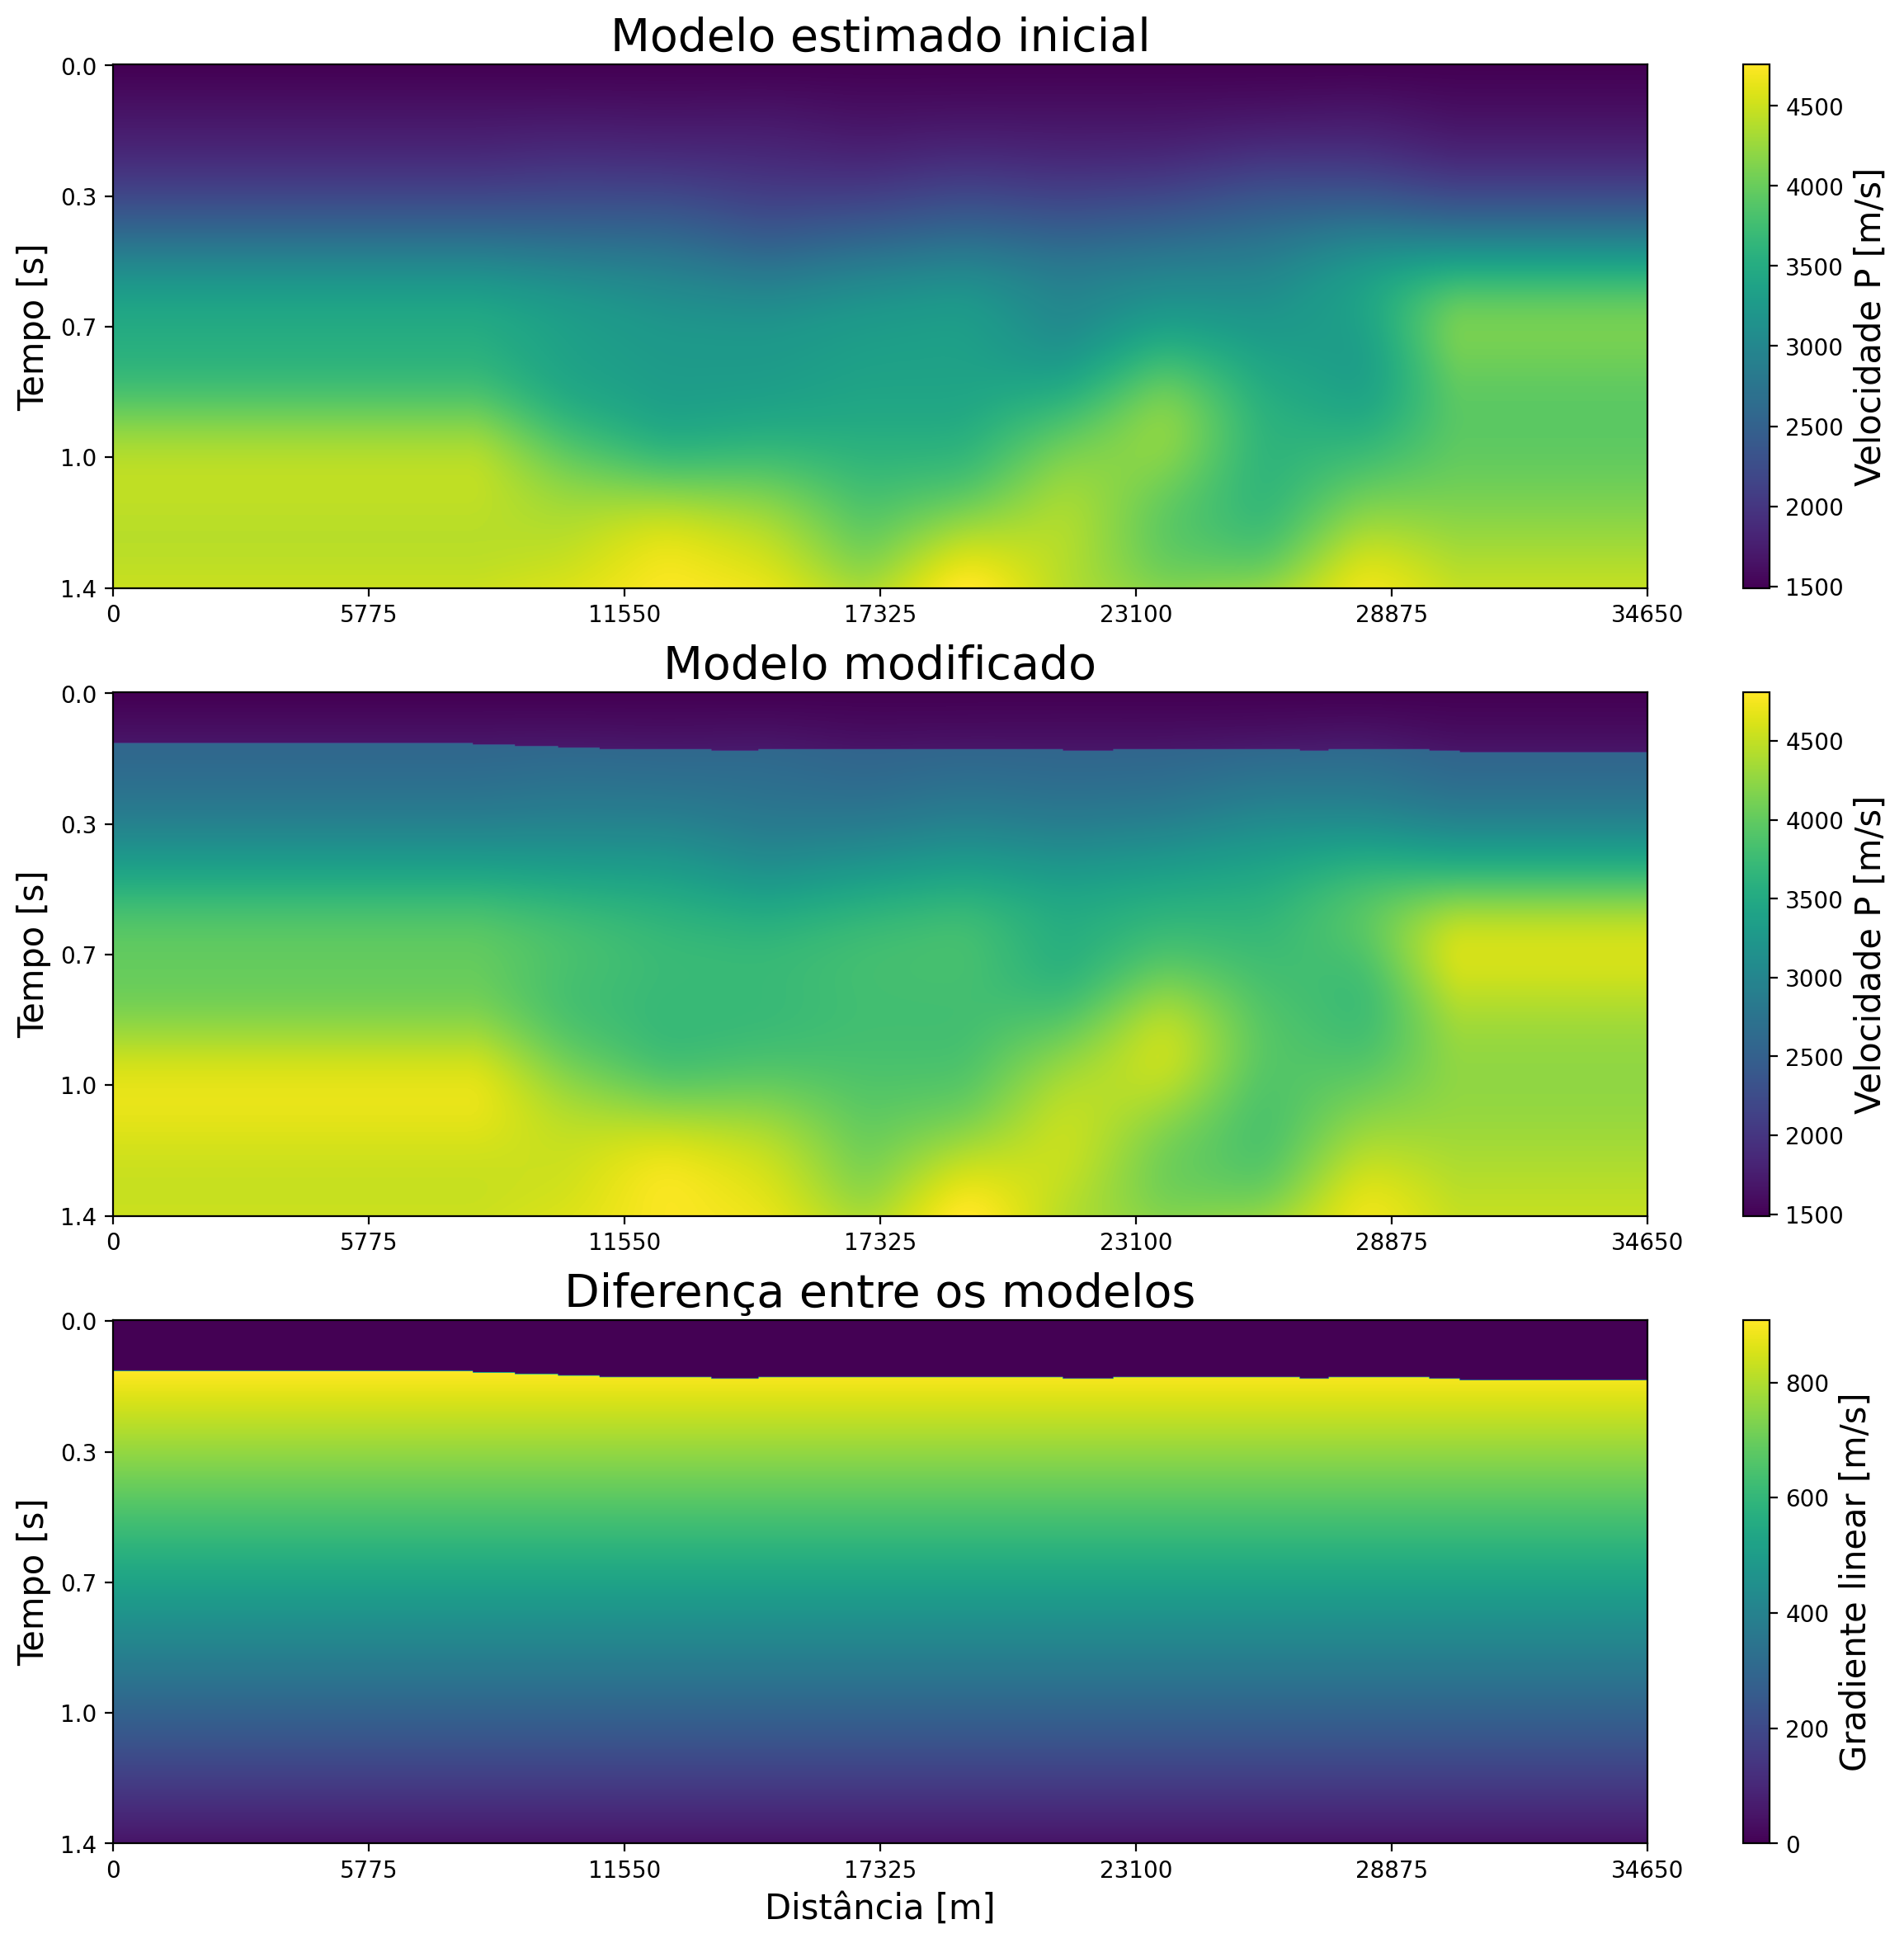
\includegraphics[width=8cm,height=6cm]{../imagens/modificationTime.png}	
			\tiny{\caption{Aplicação do gradiente de velocidades em tempo}}
		\end{figure}			
	\end{column}
\end{columns}		
	
\end{frame}
% ----------------- NOVO SLIDE --------------------------------	
\begin{frame}{Atualização do modelo de propriedades}
	\framesubtitle{Conversão tempo-profundidade do modelo atualizado}	
	
	\begin{columns}[onlytextwidth, T]
		\begin{column}{.9\textwidth}
			\begin{figure}[h]
				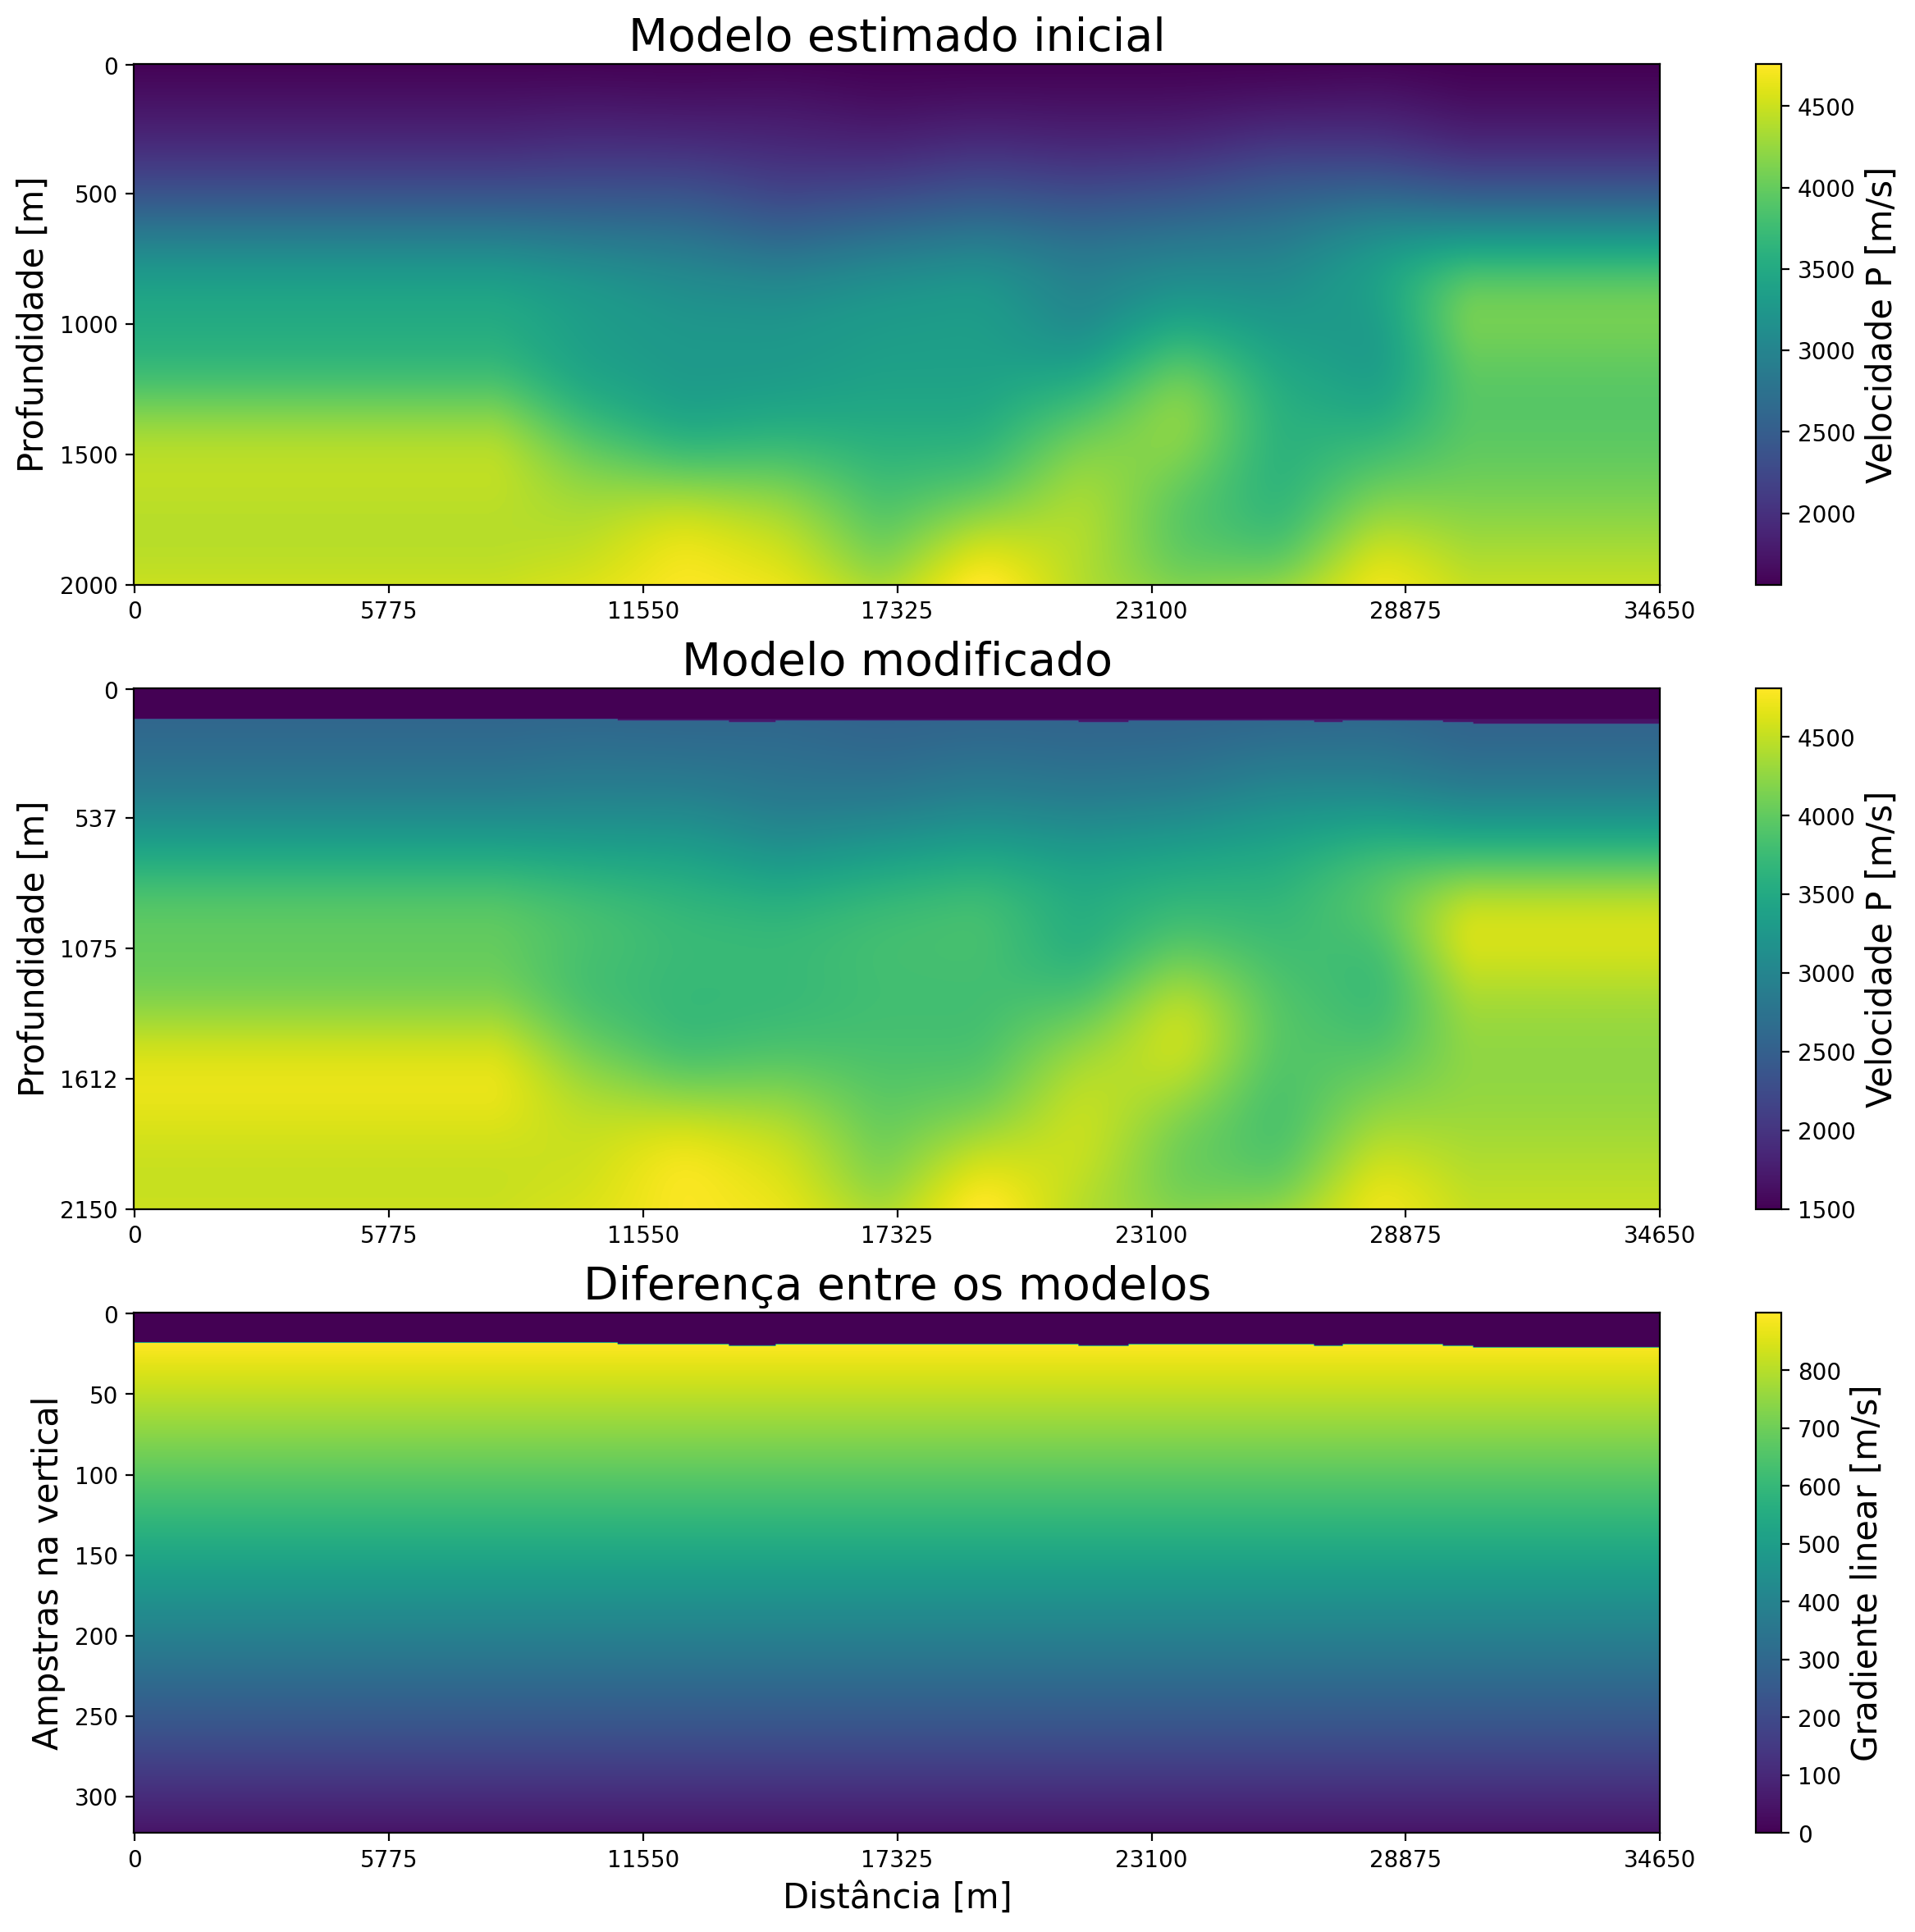
\includegraphics[width=8cm,height=6cm]{../imagens/modificationDepth.png}	
				\tiny{\caption{Conversão tempo profundidade ajustando a profundidade do fundo marinho.}}
			\end{figure}			
		\end{column}
	\end{columns}		
	
\end{frame}
% ----------------- NOVO SLIDE --------------------------------	
\begin{frame}{Gerando novos resultados}
	\framesubtitle{Seções empilhadas e migradas em tempo após a correção do modelo}	
	
	\begin{columns}[onlytextwidth, T]
		\begin{column}{.9\textwidth}
			\begin{figure}[h]
				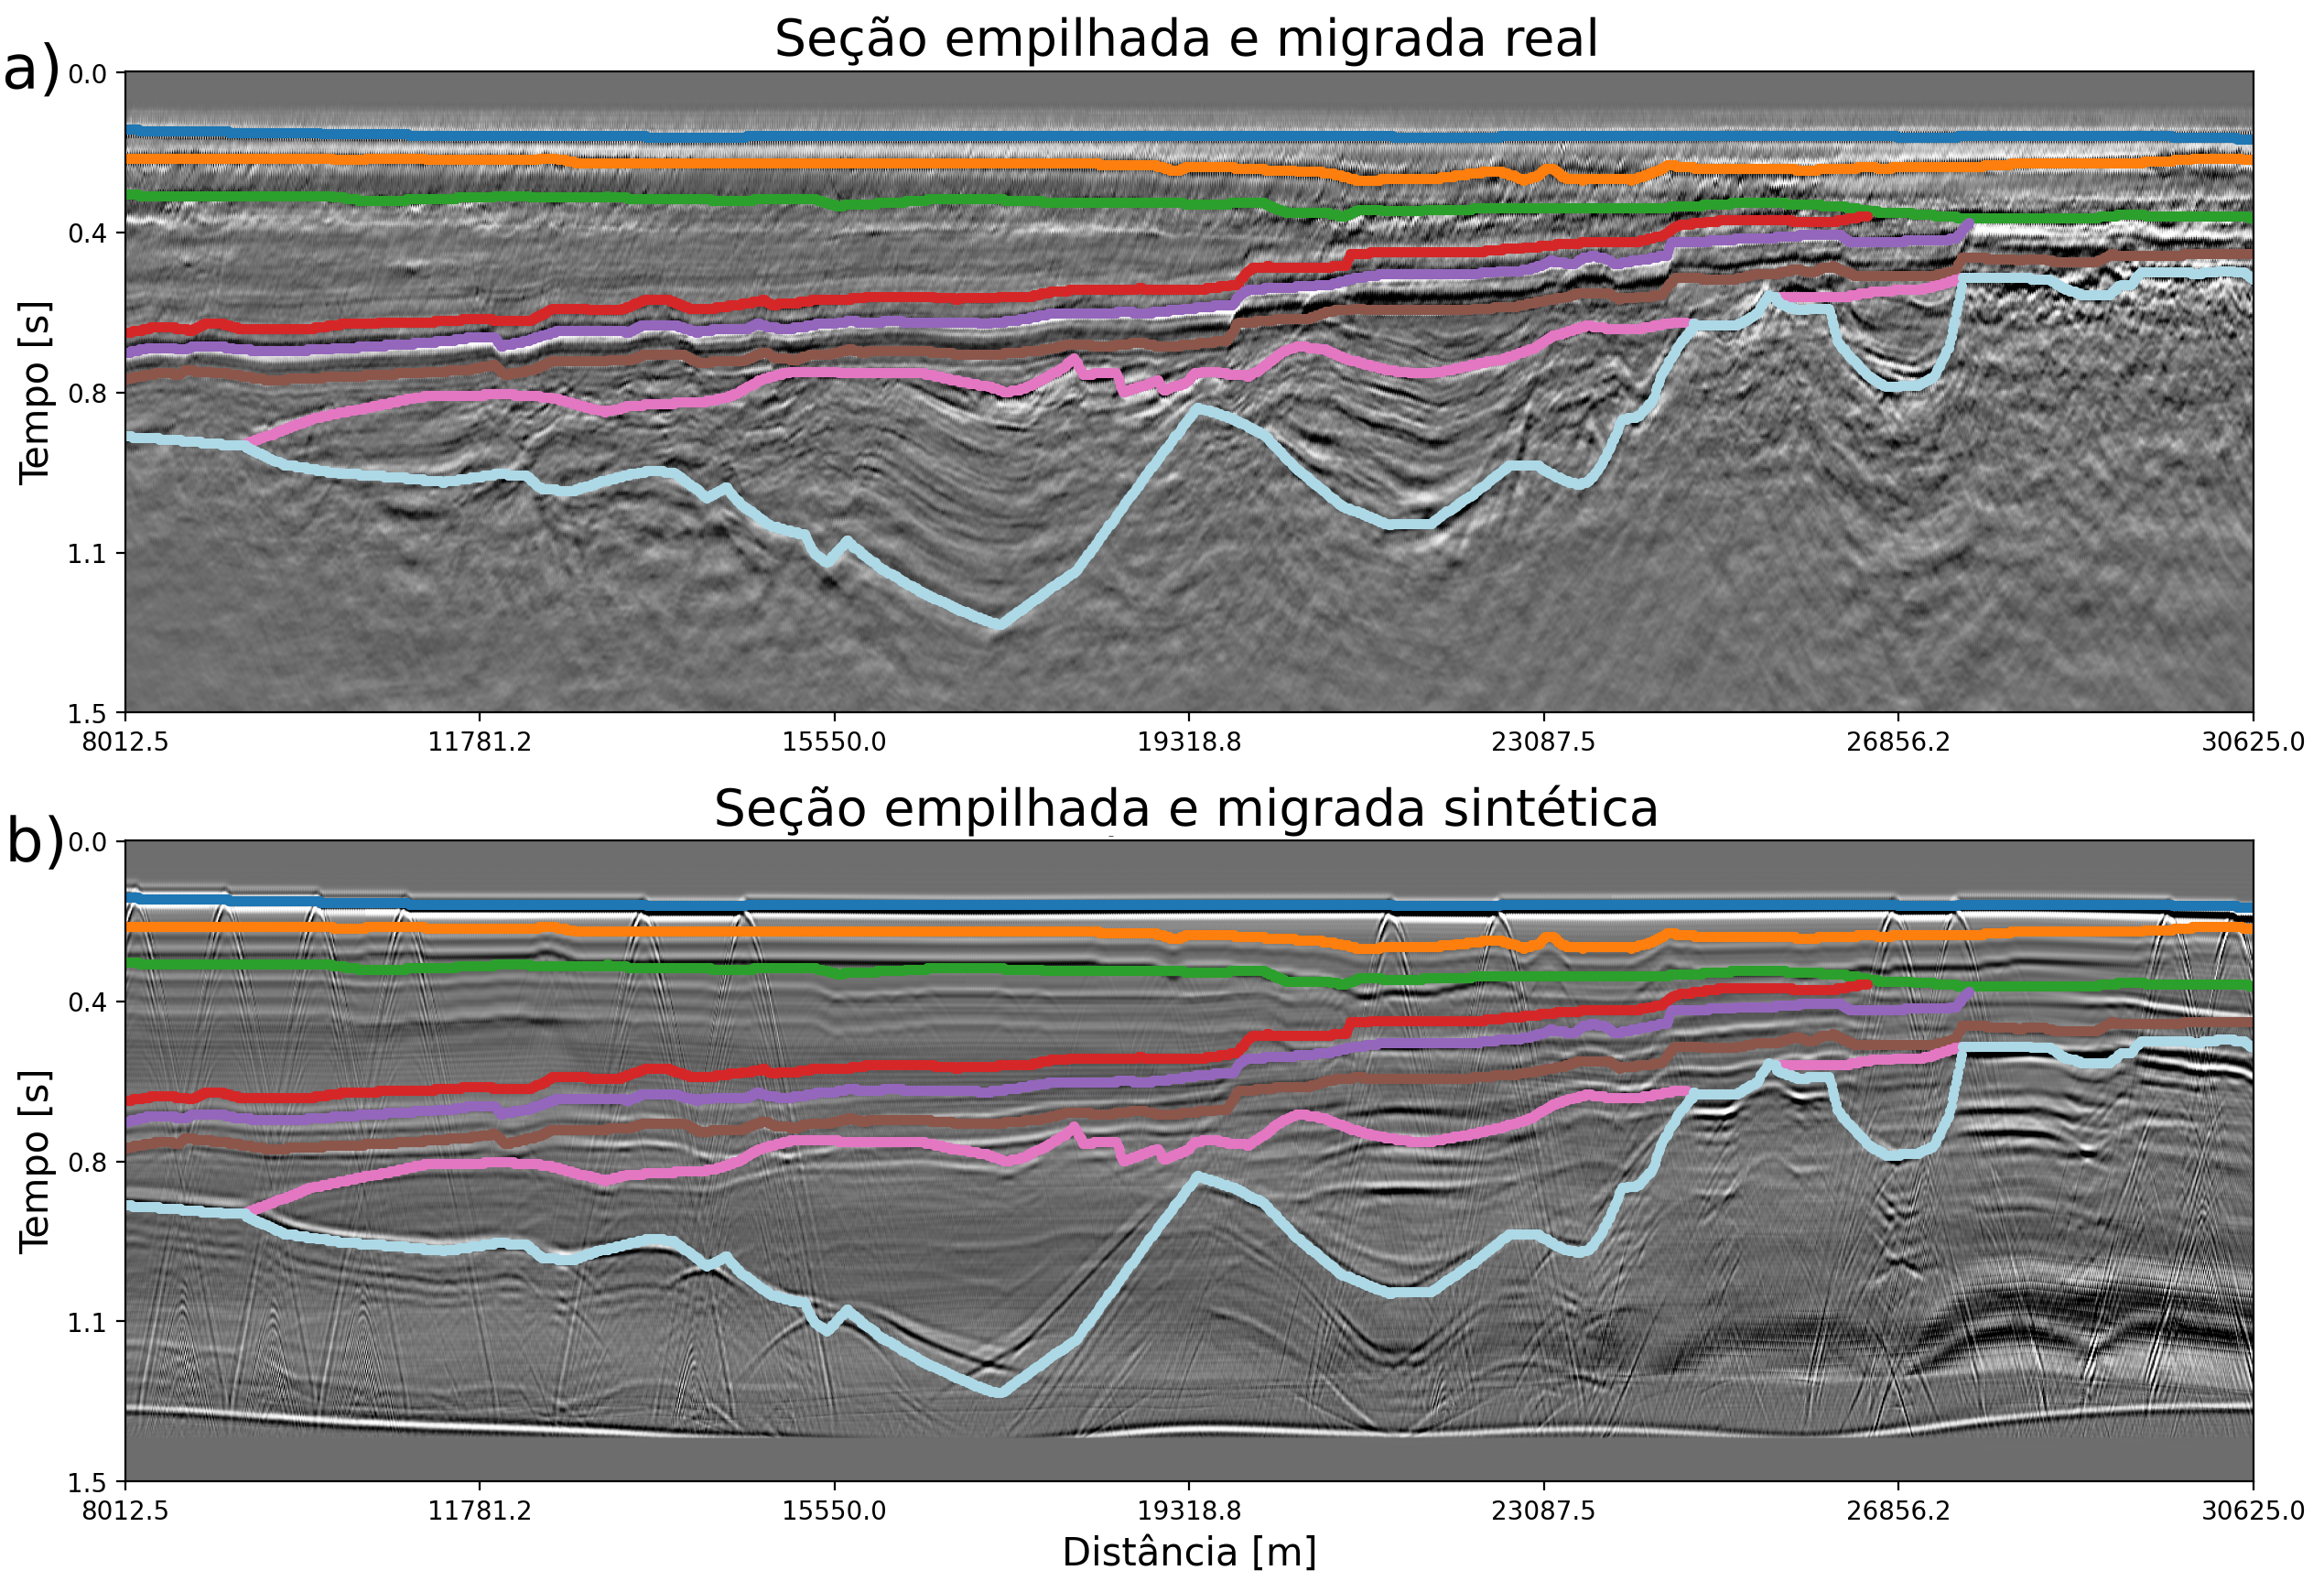
\includegraphics[width=10cm,height=6cm]{../imagens/comparision1HRZ.png}	
				\tiny{\caption{Horizontes coletados do dado real projetados. Detalhe nas reflexões agora mais ajustadas aos horizontes.}} 	
			\end{figure}			
		\end{column}
	\end{columns}	
	
\end{frame}
% ----------------- NOVO SLIDE --------------------------------	
\begin{frame}{Análise dos resultados obtidos}
\framesubtitle{Erro absoluto entre os horizontes real e sintéticos: $e_{abs}(hrz_i) = ABS(hrz_i^{obs} - hrz_i^{cal})$}	
	
\begin{columns}[onlytextwidth, T]
	\begin{column}{.9\textwidth}
		\begin{figure}[h]
			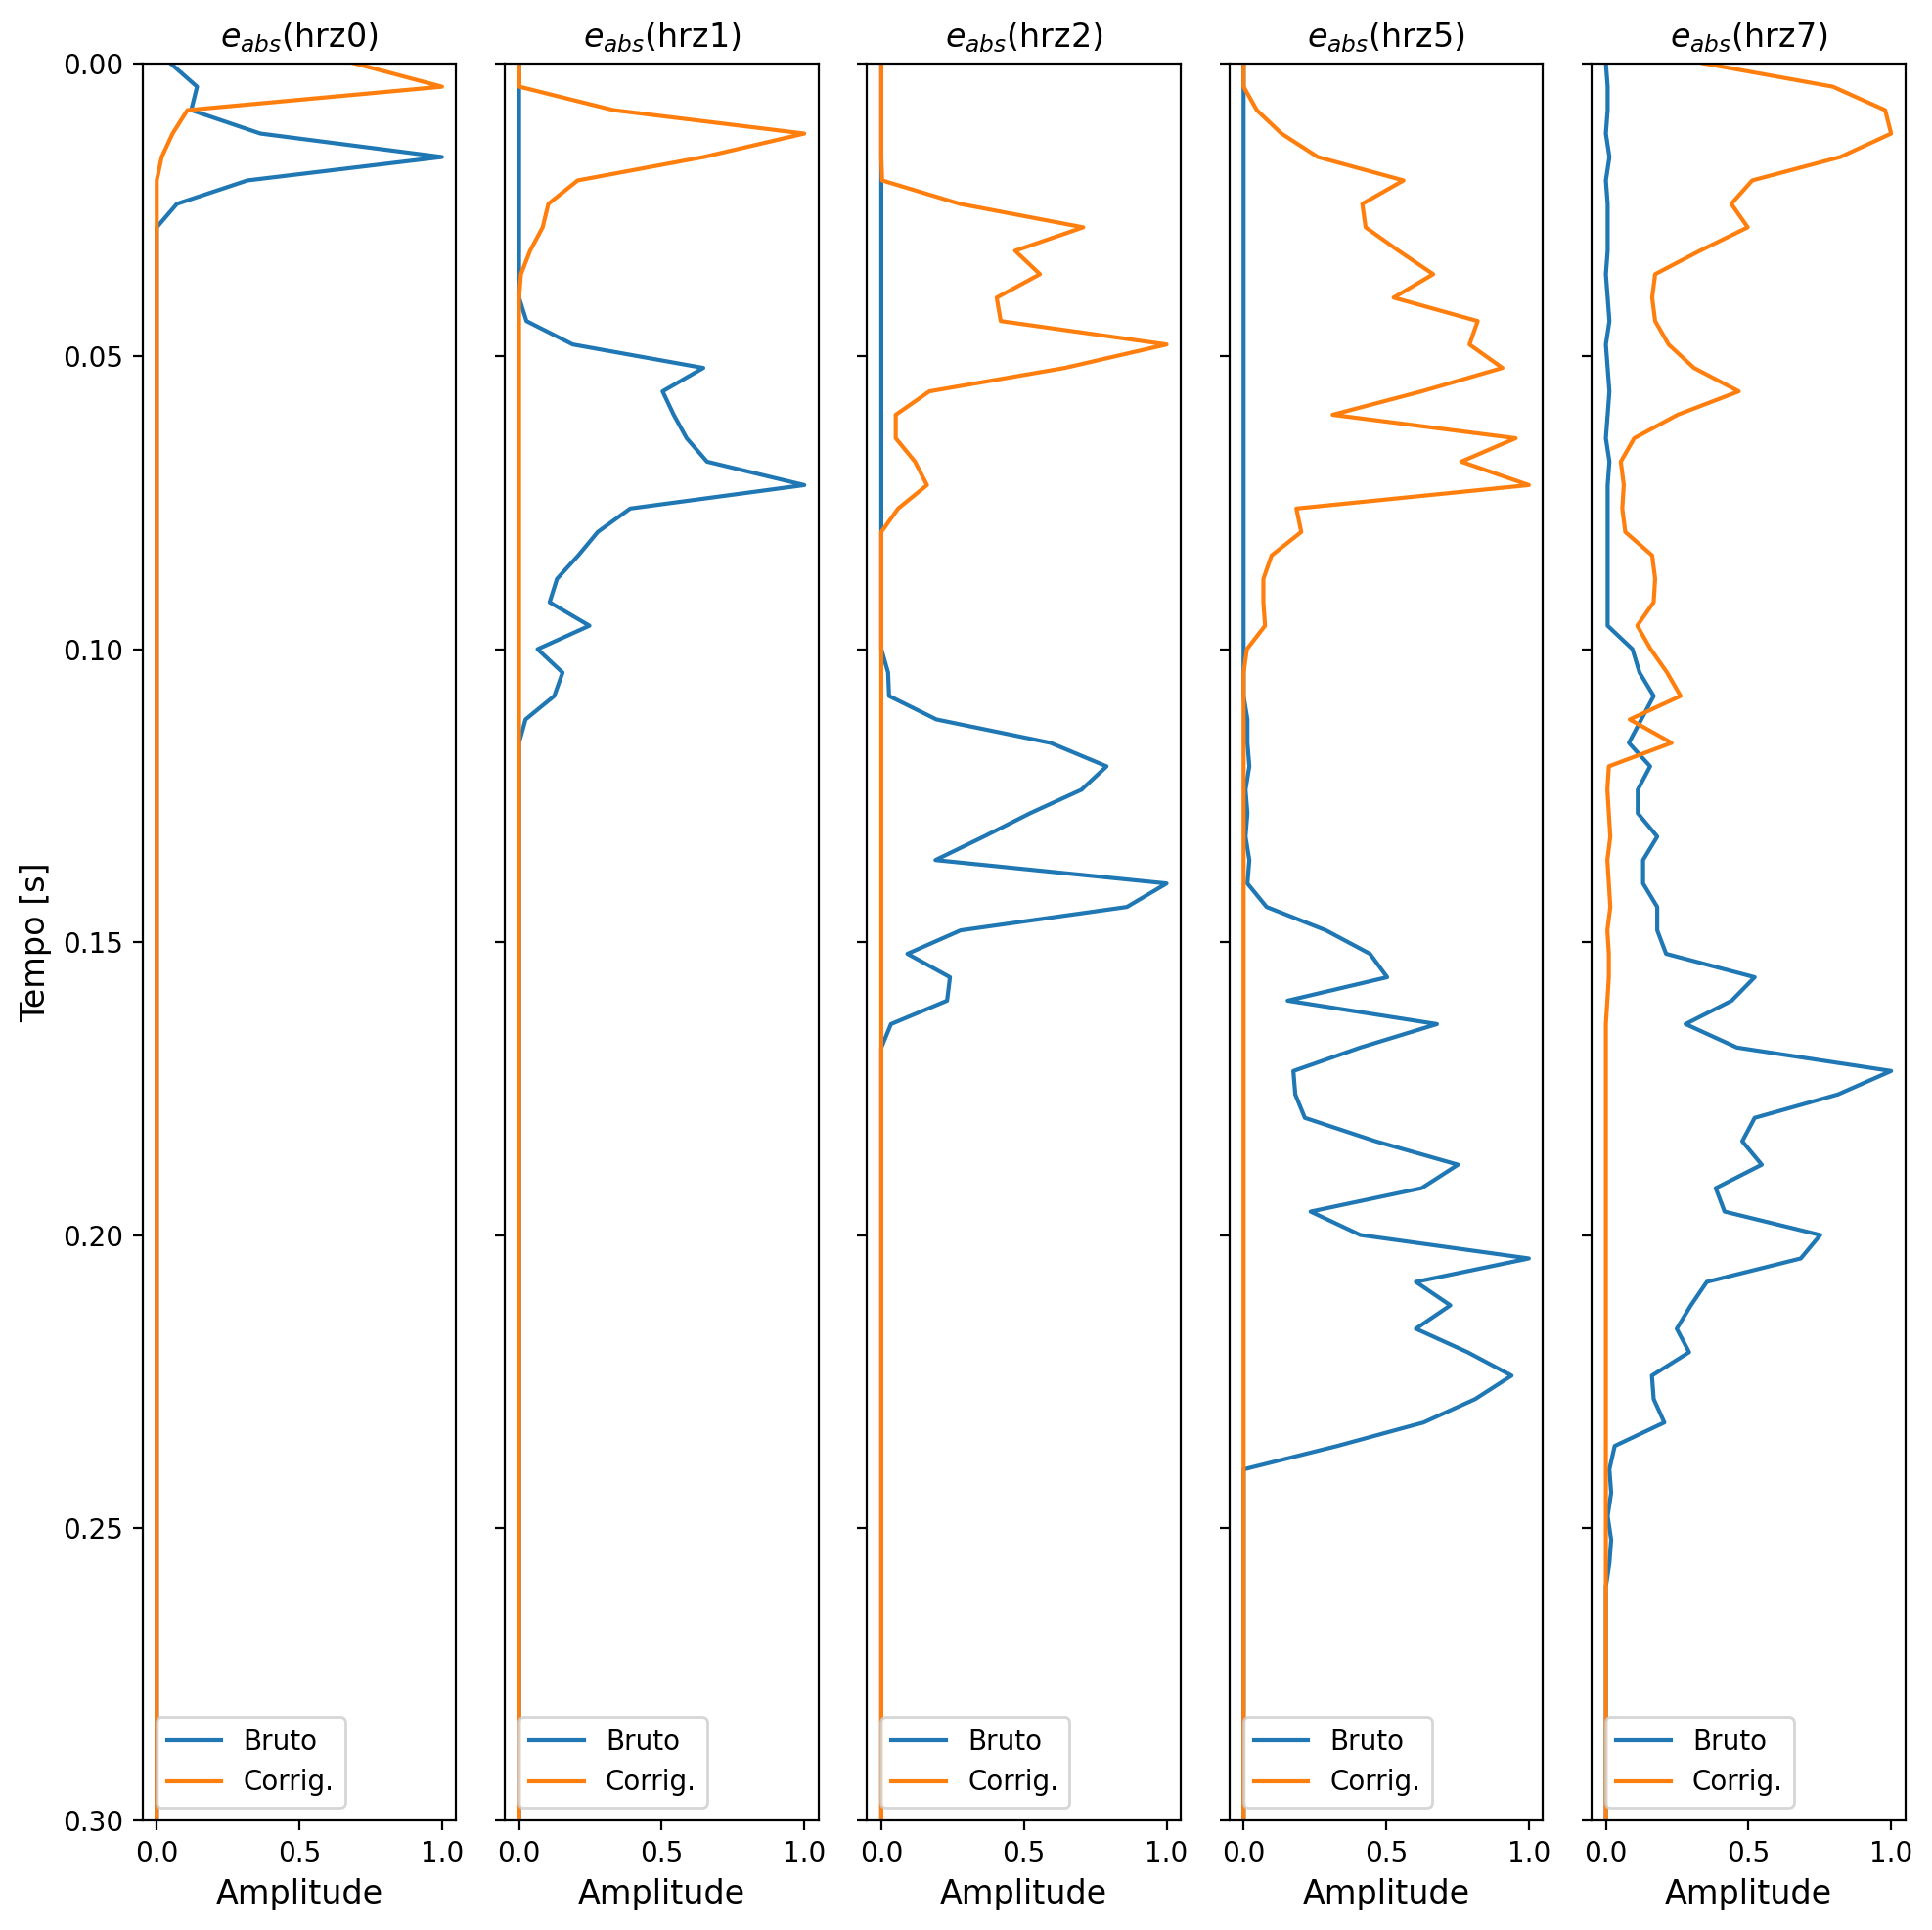
\includegraphics[width=8cm,height=6cm]{../imagens/analise.png}	
			\tiny{\caption{Histogramas com erros absolutos mostrando que, após a correção, os horizontes tem menos diferença entre real e sintético.}} 	
		\end{figure}			
	\end{column}
\end{columns}	
	
\end{frame}
% ----------------- NOVO SLIDE --------------------------------	
\begin{frame}{Comparação visual entre os horizontes}
\framesubtitle{Seções empilhadas e migradas em tempo inicial}	

\begin{columns}[onlytextwidth, T]
	\begin{column}{.9\textwidth}
		\begin{figure}[h]
			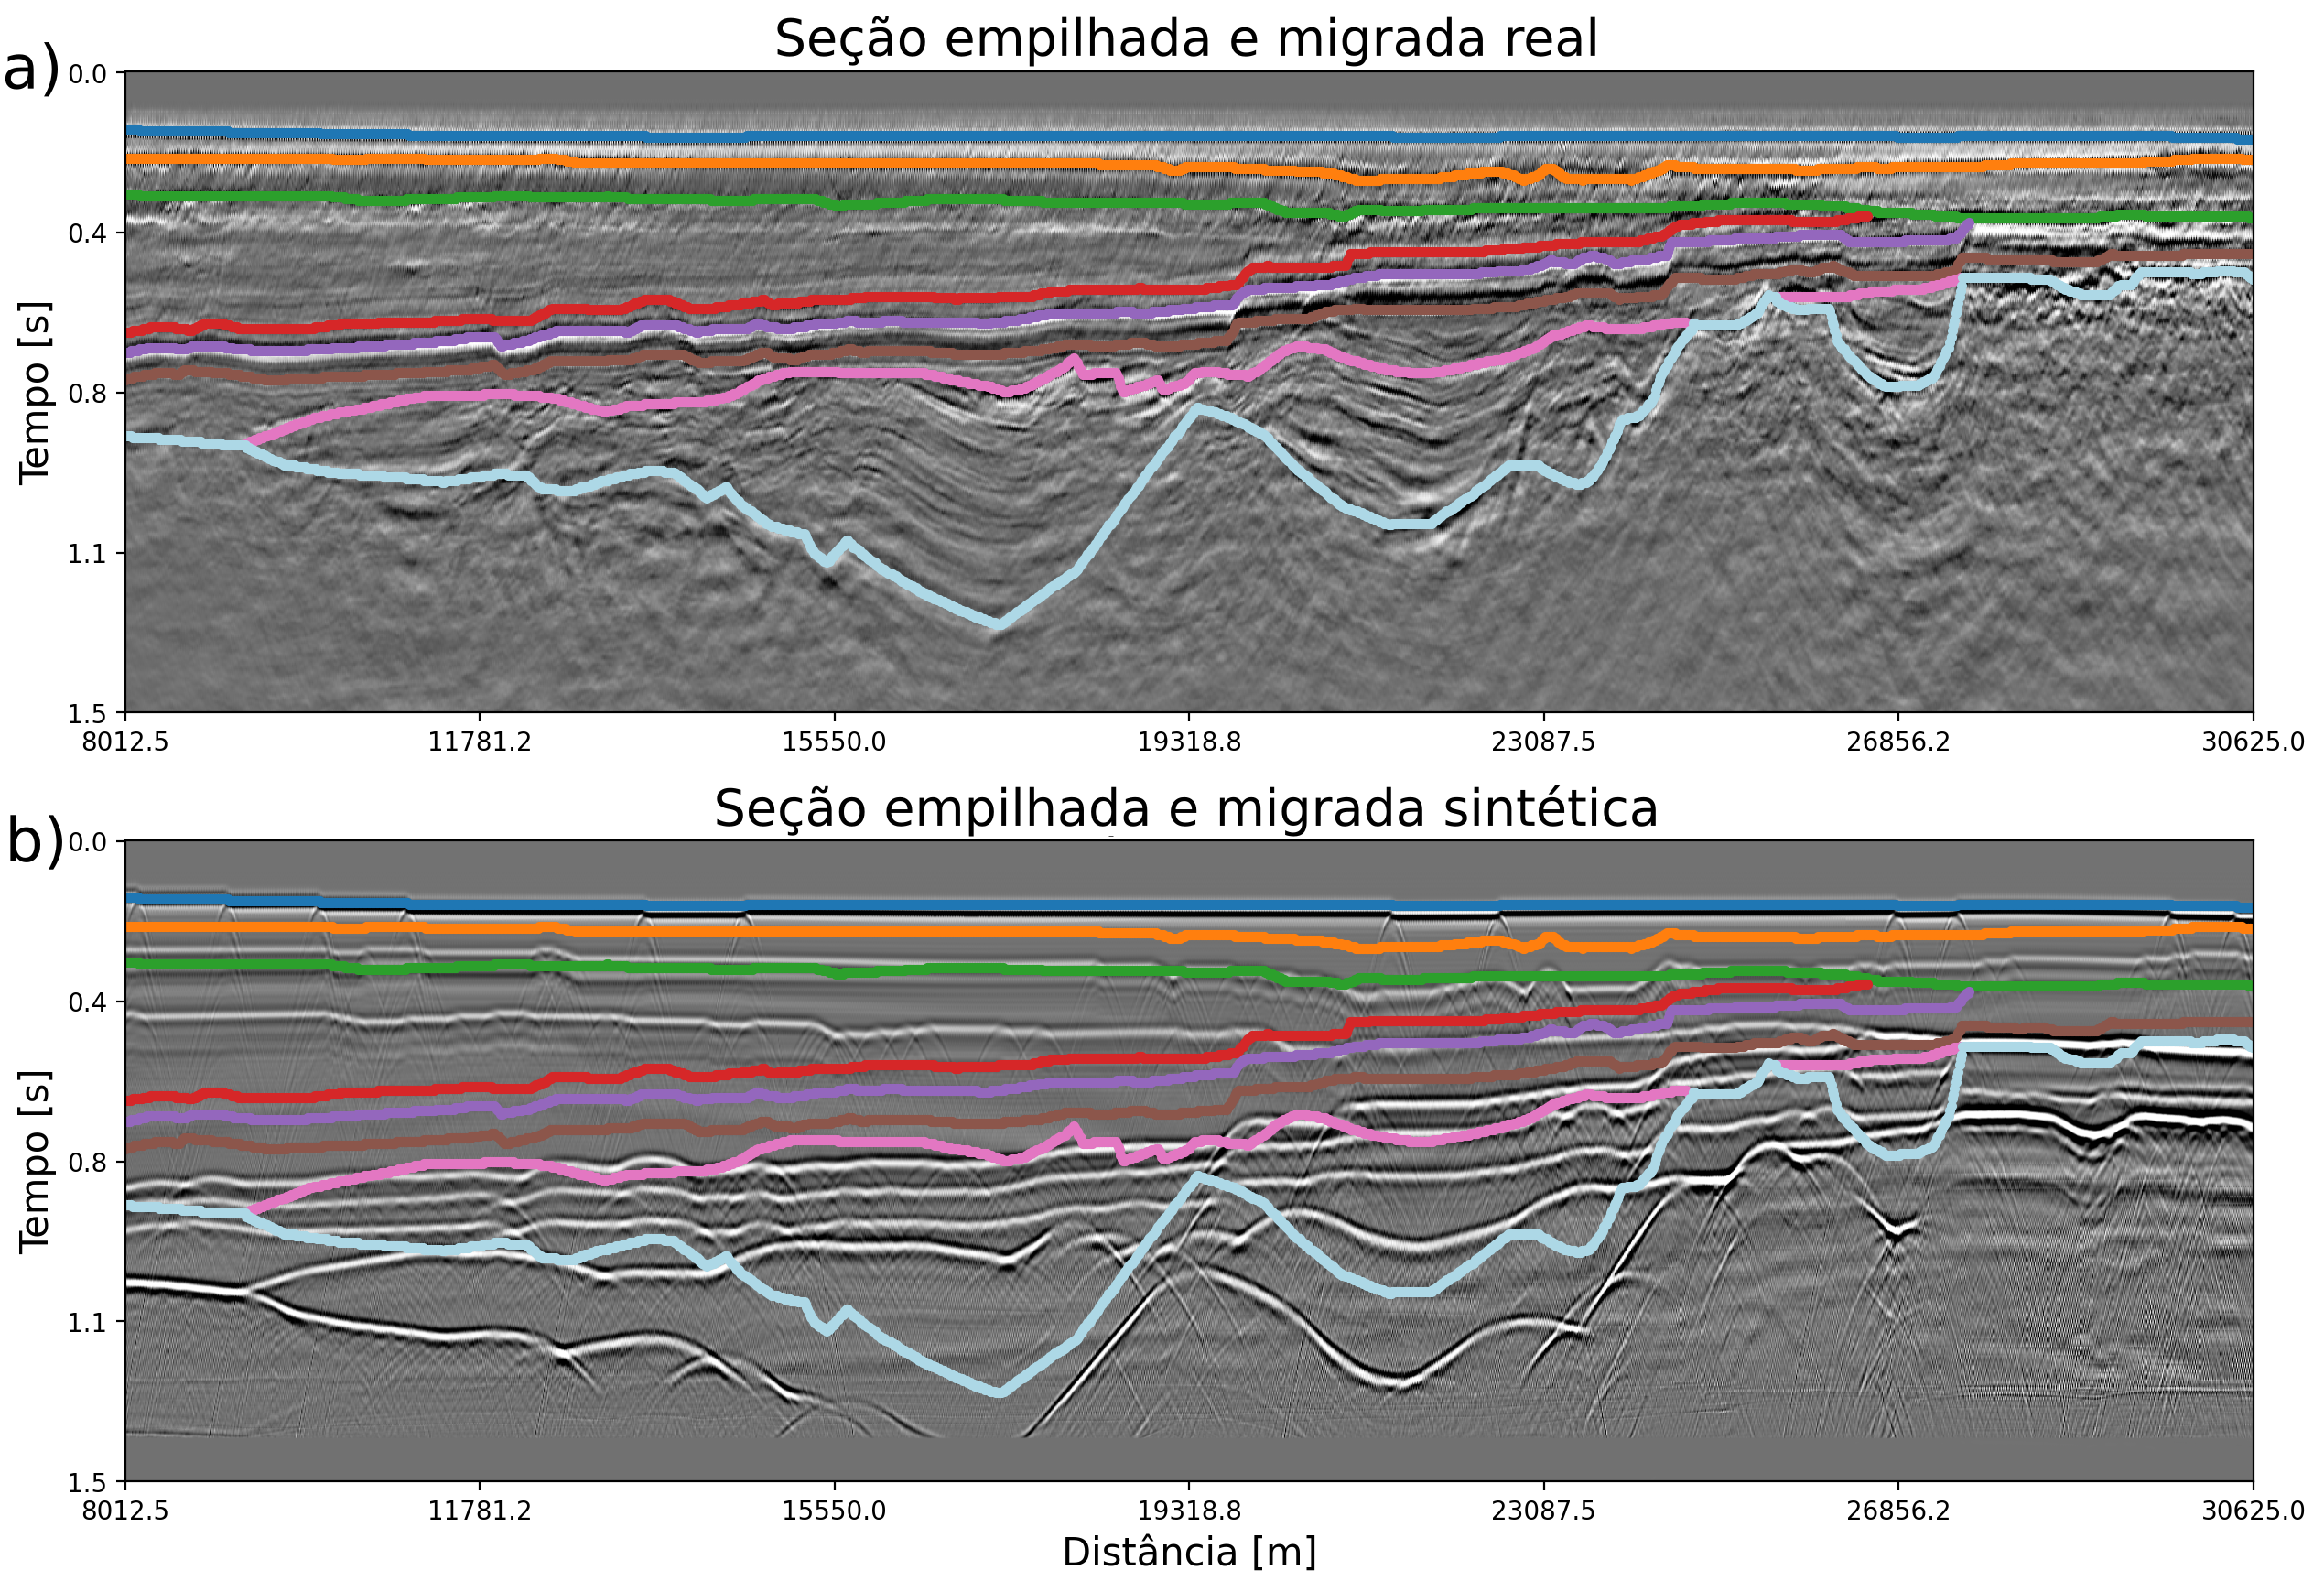
\includegraphics[width=10cm,height=6cm]{../imagens/comparisionHRZ.png}	
			\tiny{\caption{Horizontes coletados do dado real projetados na seção sintética.}} 	
		\end{figure}			
	\end{column}
\end{columns}	

\end{frame}
% ----------------- NOVO SLIDE --------------------------------	
\begin{frame}{Comparação visual entre os horizontes}
	\framesubtitle{Seções empilhadas e migradas em tempo final}	
	
	\begin{columns}[onlytextwidth, T]
		\begin{column}{.9\textwidth}
			\begin{figure}[h]
				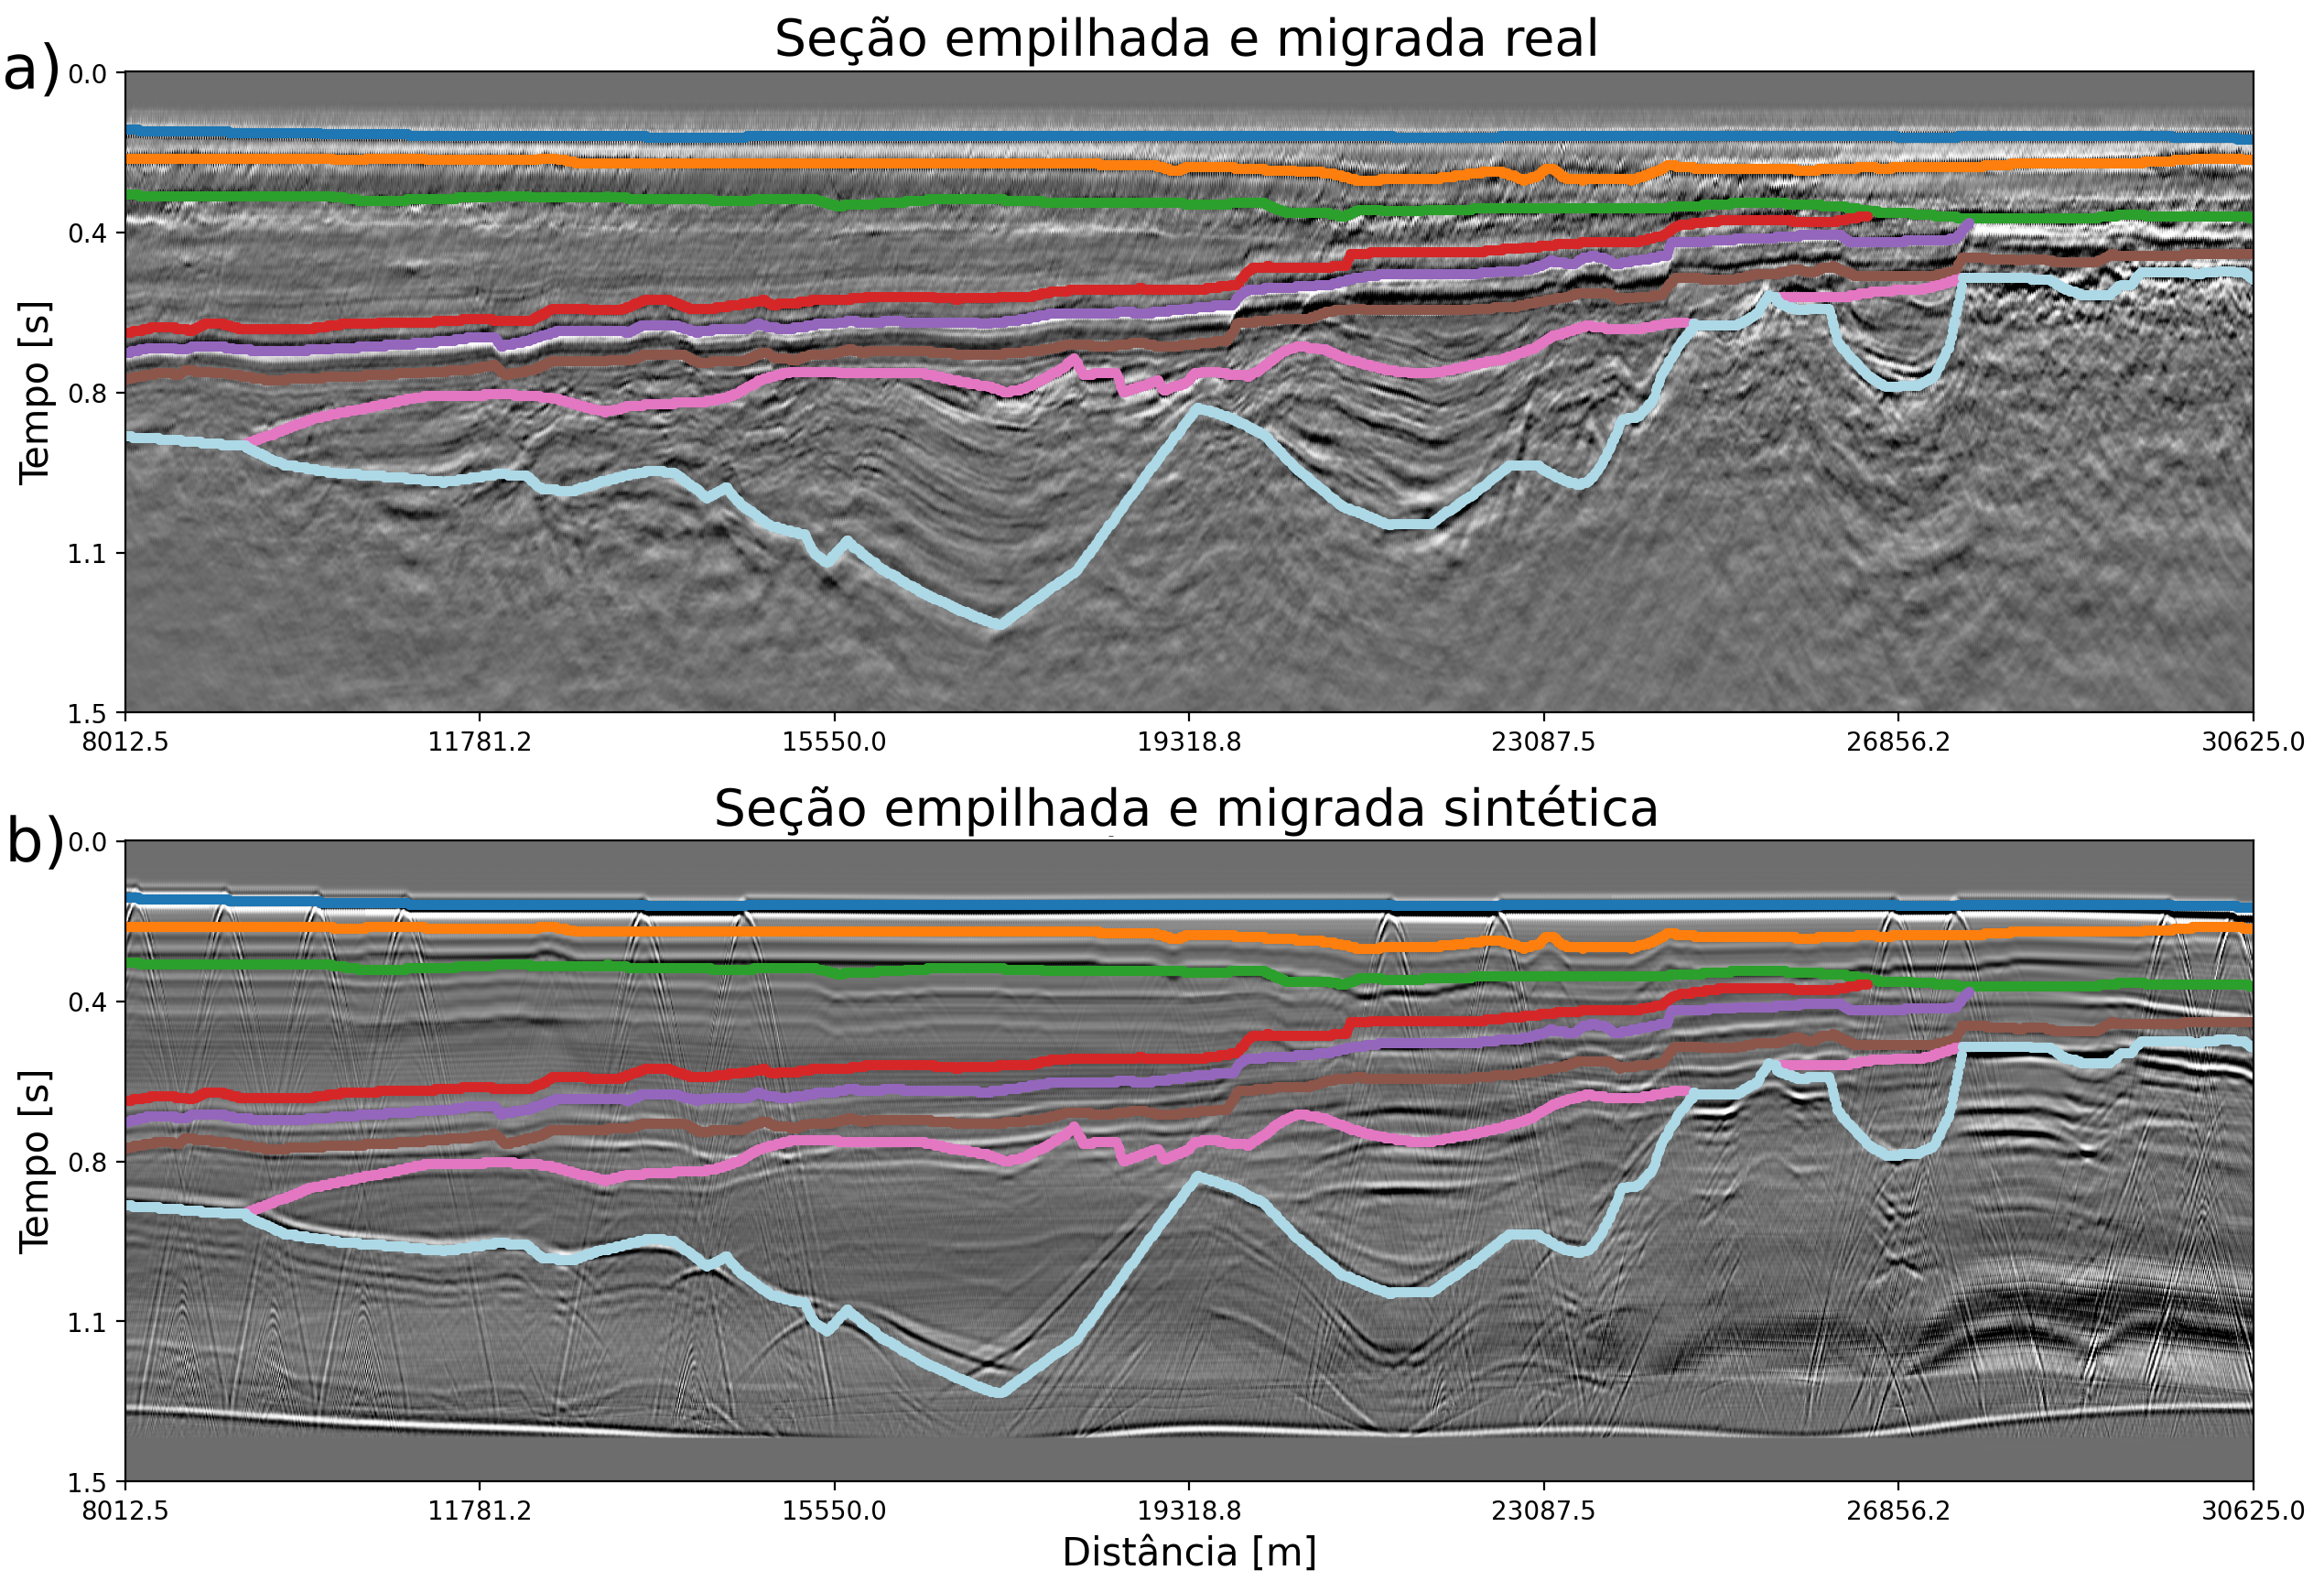
\includegraphics[width=10cm,height=6cm]{../imagens/comparision1HRZ.png}	
				\tiny{\caption{Horizontes coletados do dado real projetados na seção sintética.}} 	
			\end{figure}			
		\end{column}
	\end{columns}	
	
\end{frame}
% ----------------- NOVO SLIDE --------------------------------	
\section{Conclusão}
\begin{frame}{}
	\bigskip\bigskip\bigskip\bigskip\bigskip\bigskip
	\begin{center}
		\Huge Conclusão
	\end{center}    
\end{frame}
% ----------------- NOVO SLIDE --------------------------------	
\begin{frame}{Conclusões}
	\bigskip
	\begin{itemize}
		\item[$\bullet$] O método de análise de velocidades não identificou a anomalia rasa, mas apresentou uma boa estimativa inicial do campo de velocidades da onda P;
		
		\bigskip\pause 
		\item[$\bullet$] A atualização do modelo de velocidades foi baseada puramente nos aspectos litológicos dos perfis de poços apresentados, mostrando que o vinculo geológico é importante nos processos de construção de modelo de velocidades;
		
		\bigskip\pause
		\item[$\bullet$] A atualização em forma de gradiente funcionou razoavelmente bem pelas características geológicas estruturais da região, sendo planar e com certas continuidades laterais.  
	\end{itemize}
	
\end{frame}
% ----------------- NOVO SLIDE --------------------------------	
\begin{frame}{Trabalhos futuros}
	
	\bigskip
	\begin{itemize}
		\item[$\bullet$] Aplicar algum processo de migração em profundidade, tanto usando mecanismos de traçado de raios quanto extrapolação do campo de onda. 
	
		\bigskip\pause 
		\item[$\bullet$] Aplicar o procedimento de tomografia sísmica para ajustes pontuais do modelo $v_p$.
	
		\bigskip\pause
		\item[$\bullet$] Tentar gerar algum processo de automatização que ajuste o modelo pelos horizontes interpretados.  
	\end{itemize}
		
\end{frame}
% ----------------- NOVO SLIDE --------------------------------
\section{Referências}
\begin{frame}{Referências bibliográficas}
	\tiny
	\bibliography{referencias}
\end{frame}
% ----------------- NOVO SLIDE --------------------------------
\begin{frame}
    \bigskip\bigskip\bigskip\bigskip\bigskip\bigskip
    \begin{center}
        \Huge Agradecimentos
    \end{center}
\end{frame}
% ------------- FIM DO DOCUMENTO -------------------------------
\end{document}